% Created 2022-05-04 mié 15:06
% Intended LaTeX compiler: pdflatex
\documentclass[twoside]{article}
\usepackage[utf8]{inputenc}
\usepackage[T1]{fontenc}
\usepackage{graphicx}
\usepackage{grffile}
\usepackage{longtable}
\usepackage{wrapfig}
\usepackage{rotating}
\usepackage[normalem]{ulem}
\usepackage{amsmath}
\usepackage{textcomp}
\usepackage{amssymb}
\usepackage{capt-of}
\usepackage{hyperref}
\renewcommand\maketitle{\begin{titlepage}%
\begin{center}
       \vspace*{1cm}

       \textbf{Modelo de literariedad usando redes semánticas y n-gramas}

       \vspace{0.5cm}
        
            
       \vspace{1.5cm}

       \textbf{Jonatan Ahumada Fernández}

       \vfill
            
       Tesis para el título de Ingeniería de Sistemas
            
       \vspace{0.8cm}
     
       \includegraphics[width=0.4\textwidth]{university}
            
       Facultad de Matemáticas E Ingeniería\\
       Fundación Universitaria Konrad Lorenz\\
       Bogotá, Colombia\\
       2022
            
   \end{center}\end{titlepage}%
}

\usepackage{longtable}
\author{Jonatan Ahumada Fernández}
\date{\today}
\title{Modelo de literariedad usando redes semánticas y n-gramas}
\hypersetup{
 pdfauthor={Jonatan Ahumada Fernández},
 pdftitle={Modelo de literariedad usando redes semánticas y n-gramas},
 pdfkeywords={},
 pdfsubject={},
 pdfcreator={Emacs 27.2 (Org mode 9.4.4)}, 
 pdflang={English}}
\begin{document}

\maketitle
\tableofcontents

\section{FORMULACIÓN DEL PROBLEMA}
\label{sec:org7e70042}
\subsection{Introducción}
\label{sec:org53e6af7}

¿Qué constituye la esencia de un texto? ¿Qué diferencia un texto
considerado 'literario' de aquél que no lo es? Esta pregunta se ha
planteado en áreas como los estudios literarios y la lingüística
\cite{eijembaum2010teoria}. Particularmente, la escuela denominada
'formalismo ruso' planteó que el objeto de estudio de la literatura,
no \emph{podría} ser la belleza, la relevancia histórica o el valor
pragmático de un texto. Más bien, su objeto de estudio \emph{debe} recaer
en un aspecto más 'objetivo': su \emph{literariedad}.  Como su nombre
sugiere, los formalistas se abocaron a formular una definición
'objetiva' y 'concreta' del fenómeno literario y adoptaron los --en
ese entonces-- modernos métodos de la buyente disciplina de la
linguística.

Siendo este el caso, ¿no es, por consiguiente, factible que un
autómata pueda medir y presentar tales características presuntamente
formales con las actuales herramientas informáticas? ¿Cómo se podría
traducir la noción de \emph{literariedad} a un algoritmo que pueda ejecutar
una máquina?


\subsection{Planteamiento del problema}
\label{sec:orgb850777}
Roman Jakobson propone que la \emph{literariedad} de un texto está dada por
dos componentes de lenguaje: la diacronía y la sincronía. Estos
elementos fueron expandidos de la teoría linguística de Saussure.
Más tarde, puestos en el contexto del análisis de la poesía,
Jakobson renombró esos dos ejes como \emph{metáfora} y \emph{metonímia}, en su texto
"Linguística y poética". 



\begin{figure}[htbp]
\centering
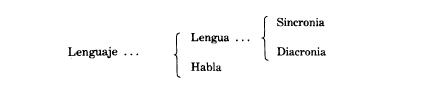
\includegraphics[width=.9\linewidth]{./assets/clasificacion_saussure.png}
\caption{Distinción entre sincronía y diacronía}
\end{figure}

¿Es posible  modelar algorítmicamente  tales conceptos? Según
Jakobson, en el estudio de la \emph{literariedad} se omite el factor emisor
y factor receptor. Tan solo se centra en el mensaje. Representado
 únicamente a través de un \emph{medio} particular: en este caso, la palabra escrita.
Es, por lo tanto,  \emph{factible} que un autómata pueda medir y presentar tales
características. 

\begin{figure}[htbp]
\centering
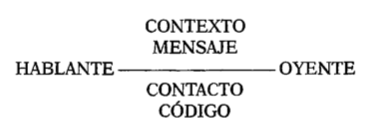
\includegraphics[width=.9\linewidth]{./assets/factores_comunicacion.png}
\caption{Factores de comunicación de Roman Jakobson \cite{jakobson1981linguistica}}
\end{figure}

Saussure ofrece ya un modelo cualitativo muy bien esbozado en teoría,
que es el que luego Jakobson utilizará para definir la literariaded.
Sin embargo, aunque existe un planteamiento cualitativo del problema,
no se halló en la bibliografía consultada un modelo computacional que
modelara el concepto y lo implementara. 

\begin{figure}[htbp]
\centering
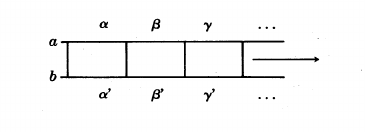
\includegraphics[width=.9\linewidth]{./assets/delimitacion_saussure.png}
\caption{Modelo cualitativo inicial expuesto por Ferdinand De Saussure tomado de \cite{eijembaum2010teoria}}
\end{figure}

Preliminarmente, se puede observar que el modelo de Saussure se
fundamenta en una estructura bastante familiar en la computación: la
secuencia \cite{alonso1945curso}. Así, el objetivo de este trabajo es modelar e implementar el
modelo de \emph{literariedad} de Roman Jakobson utilizando redes semánticas
y n-gramas.


\subsection{Justificacón}
\label{sec:org0ae1e9f}

Si bien existen infinitas operaciones realizables sobre un texto
computarizado, hay pocas que tengan un enfoque humanístico, sea
este linguístico, literario o estético. Este
enfoque busca generar una mayor comprensión del fenómeno literario,
en contraposición a los enfoques 'típicos' --y hoy en día
indispensables-- de procesamiento de lenguaje: extracción de
información, clasificación con base a un modelo predictivo, entre
muchos otros \cite{gelbukh2004}.

Más aún, dentro de este subcunjunto reducido, pocos están guiados por
aquello que Gelbuhk llama 'la ciencia fundamental'. A saber, la
linguística. En otras palabras, hay un vacío en el campo de la
linguística computacional en lo que se refiere a modelos que procuran
cuantificar esta perspectiva.

Tal vacío genera que el estudio académico de la literatura no pueda
sustentarse en datos 'duros' o ,por lo menos, cuantitativos propias
del método científico. Por otro lado, los diversas y posibles formas
de calcular la 'creatividad', la 'rima' o la 'belleza' de un texto,
propuesto por otros investigadores, pueden considerarse casuísticos,
acoplados a las objetivos y circunstancias de cada investigación en
particular, desde la perspectiva de la linguística general.

Así, se necesita un modelo de la \emph{literariedad} que exprese
concretamente la metáfora y la metonimia. Bien sea para ampliar las
aplicaciones de la linguistica computacional o para someter a
escrutinio los planteamientos de la teoría.

En esta investigación se formulará y evaluará un modelo para obtener
una medida cuantitativa para el concepto de \emph{literariedad} de Roman
Jakobson utilizando redes semánticas y n-gramas. De este modo, la
presente investigación respondería a la pregunta ¿Cómo medir
computarizadamente la \emph{literariedad} de un texto según el marco de la
lingüística de Jakobson?

\subsubsection{\textbf{Palabras clave:}}
\label{sec:org128ab57}
NLP, computational linguistics, literariness,literary theory, poetics, theory of formal method

\subsubsection{\textbf{Área de conocimiento:}}
\label{sec:orge2c6128}

Lingüística computacional

\subsection{Alcances y delimitaciones:}
\label{sec:org91316f4}

Para computar una métrica de \emph{literariedad} será necesario comparar
un \emph{corpus objetivo} con respecto a un \emph{corpus de referencia,} este
último representará el ‘uso corriente de la lengua'. La primera
limitación de este trabajo es que no se compilará un corpus propio, sino
que partirá de los de acceso libre. La mayoría de estos se encuentran en
inglés. Por este motivo, el corpus de referencia más a la mano es
WordNet, que al ser una ontología ya contiene las anotaciones necesarias
para mi objetivo. A saber, una lista de sinónimos por palabras. Por otro
lado, el corpus objetivo no tiene que estar anotado (utilizaré un
PlainTextCorpus), pero de algún modo tiene que ser razonable su
comparación con el corpus objetivo. Por ejemplo, los resultados del
modelo serían muy difíciles de evaluar si la relación entre corpus
objetivo y de referencia sobrepasa los 2 siglos, dada la naturaleza
fluida de la lengua.

La segunda limitación concierne a la formulación de los algoritmos en sí
mismos. Me limitaré a formular los modelos más naive posibles. Por
ejemplo, (retomando el ejemplo previo) dada una palabra se considerará
un sinónimo todas las palabras listadas como tal en el corpus de
referencia, sin considerar los sub-problemas que esto podría conllevar.

En general, el alcance de este proyecto es formular e implementar un
modelo general que muestre cómo sería viable implementar el concepto de
\emph{literariedad}, sin ahondar en los detalles que se desprenden de cada
fase del flujo de NLP (por ejemplo, ¿cómo tokenizar?, ¿Qué peso tendrían
las diferentes partes de una oración en el computo final, etc).

\section{OBJETIVO GENERAL}
\label{sec:orgfbe8e27}
Diseñar e implementar un modelo que, dado un corpus de texto, produzca
indicadores para el concepto de \emph{literariedad} que plantea Roman Jakobson.

\section{OBJETIVOS ESPECÍFICOS}
\label{sec:orgd65aa4b}

\begin{enumerate}
\item Construir el corpus necesario para representar el \emph{eje diacrónico}
\item Diseñar e implementar el algoritmo para calcular la \emph{metáfora} sobre un corpus
\item Diseñar e implementar algoritmo para calcular la \emph{metonimia} sobre un corpus
\item Seleccionar y unir los textos que serán procesados (corpus objetivo) por el algoritmo
\item Correr el algoritmo sobre los corpus objetivo
\item Evaluar el algoritmo de manera cuantitativa y cualitativa
\end{enumerate}

\section{MARCO TEÓRICO}
\label{sec:org3cceaf6}

\subsection{Literariedad}
\label{sec:orge0249c3}


La \emph{literariedad} es, según Jakobson, la cualidad de un objeto
literario en cuanto tal. Por lo tanto, la \emph{literariedad} no depende de
ningún factor extrínseco, como su emisor, su valor histórico, las
ventas de tal o cual libro, las citaciones, etc. La \emph{literariedad} se
da exclusivamente por atributos propios del fenómeno del lenguaje.

Para analizar la \emph{literariedad}, se deben analizar las dos operaciones
más básicas de la conducta verbal: \emph{la selección} y \emph{la combinación.}


\subsubsection{Selección (ver linguística sincrónica):}
\label{sec:orge9c0dc1}

La selección estudia qué palabra selecciona un hablante entre las
palabras existentes de la lengua, más o menos similares y hasta
cierto punto equivalentes. La selección se basa en la sinonimia o
antonimia de una palabra. En otros términos, en su semántica.


\subsubsection{Combinación (ver linguística diacrónica):}
\label{sec:orgb9c5def}

La combinación estudia el "entramado de la secuencia" de un
mensaje. Es decir, el mensaje considerado como una secuencia
temporal y/o ordenada de palabras. La combinación se basa en la
proximidad o, en otras palabras, en la relación de una palabra con
la que la sucede o antecede en un mensaje.



\subsection{Poética}
\label{sec:orgbadd3b8}
La poética procura responder a la pregunta de ¿qué hace que un
mensaje (verbal o de otra naturaleza) sea una obra de arte? Lidia
principalmente con cuestiones estéticas del lenguaje. Sin embargo,
para hacer un analisis exhaustivo, la poética debe hacer uso de la
linguística, puesto que esta última estudia el lenguaje en todo su
conjunto. La \emph{literariedad} podría, entonces, considerarse un
concepto enmarcado en la poética, porque se preguntá qué hace que
un texto sea literario y por qué es distinto de otro que no lo es.

\subsection{Linguística}
\label{sec:org1ad347f}

La lingüística es la ciencia que estudia el lenguaje.
Tradicionalmente, esta ciencia se subdivide en las ramas de fonética,
fonología, morfología, sintaxis, semántica y pragmática.

La lingüística es un campo de estudio interdisciplinar e involucra
disciplinas heterogéneas como la lógica y la neurolingüistica. Sin
embargo, se considera que hay un núcleo común llamado \emph{linguística
general}.

\subsubsection{Lingüística General:}
\label{sec:orgd477cb3}

Se conoce como lingüística general al paradigma lingüístico
establecido por Ferdinand De Saussure, también llamado \emph{modelo
diferencial del lenguaje}.

El modelo diferencial se caracteriza porque propone dos ejes
principales existentes en todo fenómeno lingüístico: el \emph{eje de
sincronía} y el \emph{eje de diacronía}.

Estos dos ejes son la base de lo que Jakobson considera \emph{selección} y
\emph{combinación}.


\subsubsection{Lingüística sincrónica}
\label{sec:orge309dc2}

La linguística sincrónica se ocupa de las
operaciones que realiza un hablante, sean lógicas o psicológicas,
para formar un sistema linguístico. En el
marco de esta investigación el \emph{eje sincrónico} se referirá a las
posibles palabras que un hablante pudo haber seleccionado para
expresar una misma idea. Por ejemplo, para referirse a un
niño, un hablante puede utilizar la las palabras "niño", "chico",
"jovencito", o "párvulo".


\subsubsection{Lingüística diacrónica}
\label{sec:orgfe4dc43}

La linguística diacrónica estudia los cambios sucesivos en el
lenguaje, producidos por la actividad constante del \emph{eje
sincrónico}. En la perspectiva de Jakobson, un \emph{mensaje} tiene en
sí mismo un eje diacrónico. Tal eje mide la similaridad entre cada
término del mensaje entindido como secuencia. Un ejemplo se puede
apreciar en la oracion "I like Ike". An esta se evidencia una
repetición de sonidos similares: [ay layk ayk]. La similaridad, no
está dada por el significado, sino que aquí se proyecta a lo largo
del tiempo:"(\ldots{}) para decirlo de un modo más técnico: todo
secuencia es un símil."

\subsection{Lenguaje}
\label{sec:orgedaa72a}
En términos simples, el lenguaje es la facultad de formular y
comprender signos o símbolos, ya sean hablados, escritos,
imágenes, etc.  En otros términos, el lenguaje es una capacidad
general. Sin embargo, para Saussure, la lengua tiene una
característica doble: que es al mismo tiempo un sistema
establecido y la constante evolución de tal sistema. Estos dos
componentes son la \emph{lengua} y el \emph{habla}.

\subsubsection{Lengua}
\label{sec:org71f57a2}

La lengua (\emph{langue}) es uno de los dos componentes del
\emph{lenguaje}.  La lengua es fenómeno social y se equipara a una
\emph{cristalización} o un producto de la suma de asociaciones entre
conceptos e imagenes acústicas en la mente de los hablantes. Por
ejemplo, la lengua es lo que permite que dos hablantes bogotanos
puedan asociar en su mente el sonido de la palabra "chino" con el
concepto de "niño" o "infante", mientras que en otras partes del
mundo hispanohablante no existe tal asociación común.
En términos simples, la lengua es un entendimiento compartido de
lo que significan las palabras. La contraparte de la lengua,
es el habla. 

\subsubsection{Habla}
\label{sec:org1962227}
El habla (\emph{parole}) es uno de los dos componentes del
\emph{lenguaje}. El habla es el uso individual de la lengua.
Evidentemente, cuando un individuo habla puede modificar
la lengua a su antojo, porque posee la facultad del
lenguaje y jamás meramente repite el consenso de la lengua.
Como consecuencia de esto, la lengua está continuamente
siendo transformada por el habla. En términos simples,
la suma de los actos individuales de comunicacion lentamente
terminan por transformar el consenso social sobre cómo
hablar.  Por este motivo la linguística debe tener una
perspectiva doble: \emph{diacrónica} y \emph{sincrónica}.


\subsection{Lingüística Computacional}
\label{sec:org61372ed}

Es la intersección entre la computación y la lingüística. Por lo
general, se preocupa acerca de cómo procesar automáticamente el
lenguaje natural, para lo cual genera modelos lingüísticos sobre los
que luego se pueden definir operaciones comunes \cite{gelbukh2004}.


La lingüística computacional es en sí misma un campo amplio y
heterogéneo(ver \ref{fig:org85951af}).
Este trabajo se incribe concretamente dentro del procesamiento
del lenguaje natural \ref{sec:orgae18d21}, y tiene un fuerte componente de
lingüística general .

\begin{figure}[htbp]
\centering
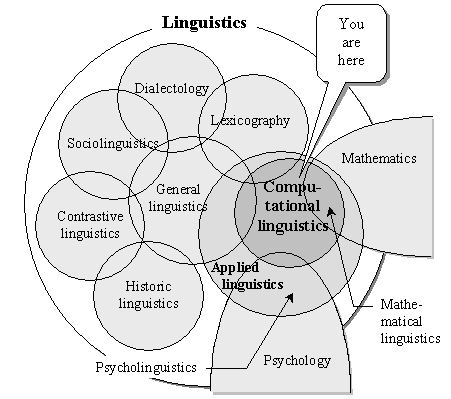
\includegraphics[width=.9\linewidth]{./assets/mapa_linguistica.png}
\caption{\label{fig:org85951af}Relación de linguística computacional con otras areas tomado de \cite{gelbuhk2004}}
\end{figure}


\subsection{NLP}
\label{sec:orgae18d21}
El procesamiento del lenguaje natural (NLP, por sus siglas en
inglés), es a menudo considerado sinónimo con la lingüística
computacional \cite{gelbukh2004}.  Sin embargo, el NLP se refiere
concretamente a la aplicación práctica de la linguística
computacional para procesar automáticamente (a menudo en enormes
cantidades) mensajes de lenguaje natural y obtener de estos alguna
información o un acción sin intermedio de un humanano.

En este trabajo, se utilizan algunas herramientas típicas del
NLP, como corpus, N-gramas, tokenización y vectorización, explicadas
en a continuación. Sin embargo, es necesario hacer explítico de
que se parte una herramienta computacional en particular: NLTK.

\subsubsection{NLTK}
\label{sec:org94dbfa6}
El Natural Language Toolkit (NLTK) es un módulo de Python que
ofrece una interfaz para tareas comunes en la lingüística
computacional. La ventaja principal de NLTK es que se considera a
sí mismo un \emph{toolkit}. Esto significa que no impone una estructura
de procesamiento definida a la vez que ofrece un extenso abanico de
herramientas, tales como: tokenizacion, filtros, generación de
n-gramas, análisis sintáctico de oraciones, entre otras.

Se seleccionó esta herramienta porque no impone una estructura
rígida en cuantó que cómo procesar el texto, lo que la hizo
idónea para perseguir los objetivos interdisciplinares de esta
investigación. Es

\subsubsection{N-gramas}
\label{sec:orge84f8e7}

Los N-gramas son una herramienta común en el procesamiento
de lenguaje natural y tienen diversas aplicaciones. Desde sus
inicios \cite{manning1999foundations}, los n-gramas se han
utilizado para capturar la noción de 'contexto' o 'historia'
dentro de una secuencia de tokens. Así los n-gramas, forman
una tupla o secuencia de palabras dentro de una secuencia
o texto más grande y, delimitado el tamaño o nivel del
n-grama, los términos circunscritos dentro del n-grama
se entienden como variables aleatorias dependientes entre sí.

Así, los n-gramas se utilizán para tratar de predecir alguna
característica con base en algún otro componente del n-grama,
utilizando las teorías de cadenas de Markov.

En este trabajo, los n-gramas se utilizan meramente
como una herramienta que captura la 'memoria' o 'relación'
de dos palabras adyacentes dentro de un mensaje. No se
utilizarán funciones de probabilidad, sino que se hará
un cálculo de similitud utilizando el algoritmo descrito
en la sección  \ref{sec:org002dd7e}, utilizando
n-gramas de nivel 2 o \textbf{bigramas}.


\subsubsection{Tokenización}
\label{sec:orga78551e}
La tokenización es el proceso mediante el cual se separa la entrada
de un programa NLP en unidades de análisis más pequeñas llamadas
\textbf{tokens}. Un token puede ser una palabra, aunque no necesariamente
lo es. Por ejemplo, puede ser un lexema, un signo de puntuación
o una unidad sintáctica (un constructo sujeto - verbo, por ejemplo)
\cite{manning1999foundations}. El resultado de la tokenización
dependerá, por lo tanto, de los objetivos de la investigación.

En esta investigación se tokenizará siguiendo la noción de
palabra gráfica (\emph{graphic word}). Esto simplemente se refiere
a que cada token corresponde a una palabra separada por un espacio,
incluyendo signos de puntuación y otros caracteres alphanumericos.




\subsubsection{Vectorización}
\label{sec:org052bd77}
La vectorización es el proceso de tomar una característica o medida
y representarla como una secuencia números reales, como un vector. A menudo,
tal representación permite visualizar las características en un espacio
vectorial, aunque la visualización no es la ventaja crucial.

La vectorización es una técnica utilizada a lo largo de muchos
dominios y tiene una larga historia en el proceso de transformar
un concepto a una entrada que sea interpretable por una máquina
\cite{jha_abhishek_vectorization}.  Continuamente, catalizadas por
el auge del Machine Learning, se desarrollan técnicas de
vectorización que ayudan a hacer los cálculos de similitud entre
vectores más eficientes, dependiento del objetivo. Un buen
ejemplo es el desarrollo del modelo de Google, que
codifica las palabras de tal forma que agiliza el cálculo
de similitud entre conceptos, conservando la noción
de múltiples grados de similaridad \cite\{\{mikolov2013efficient\}.

En este trabajo, la técnica de vectorización utilizada es
la \emph{bag of words}, que es una técnica basada en la \textbf{frequencia}.

\subsubsection{Bag of words}
\label{sec:orgddd42e7}

Es una técnica de vectorización frecuentemente utilizada en NLP.
Se considera de complejidad sencilla, pero funciona exitosamente
en muchos casos de uso. Involucra 3 fases: tokenización, creación de vocabulario y,
finalmente, creación del vector.

Su funcionamiento es el siguiente: una vez se tiene el la entrada
tokenizada se construye un \emph{vocabulario}.  Este es set de cada
palabra utilizada en la entrada.  Luego, se procede a asociar a
cada palabra del vocabulario a su frecuencia en el texto, con lo
cual se obtiene un histograma de palabras. En la última etápa,
usualmente se utiliza una matriz llana en la que cada fila
corresponde con una oración y cada columna representa una entrada
en el vocabulario \cite{jha_abhishek_vectorization}.

No obstante, para en este trabajo no se utilizará este enfoque
tradicional.  Sino que el proceso de vectorizacións seguirá los
pasos descritos en la sección \ref{sec:org002dd7e}. Sin embargo,
es necesario mencionar que la técnica de bag of words conlleva
a los siguientes supuestos: 1) se asume que el orden de las
palabras en la entrada no importa, tan solo la frecuencia
de cada entrada y 2) la existencia de las palabras en el
vocabulario es indenpiente una de la otra.  
\subsubsection{Corpus}
\label{sec:org136a4ac}


Un corpus es una colección de textos auténticos que pueden ser
leídos por una máquina. Estos pueden estructurarse de muchas
formas, dependiendo de los objetivos de la investigación
\cite{indurkhya2010handbook}. Por ejemplo, pueden ser aislados (una
colección arbitraria), categorizados (una colección escogida según
algún criterio), temporales (una colección organizada
cronológicamente) o solapados (un documento puede pertenecer a
varias colecciones) \cite{bird2009natural} (ver figura
\ref{fig:orgfb89153}). Además, el formato del corpus varía
significativamente de acuerdo al objeto de la investigación. Por
ejemplo, si se desea hacer un análisis sintáctico (de la estructura
de una oración), se debe hacer un corpus anotado con POS (Part Of
Speech tag); para hacer un análisis pragmático se utiliza una
anotación pragmática, etc.



\begin{figure}[htbp]
\centering
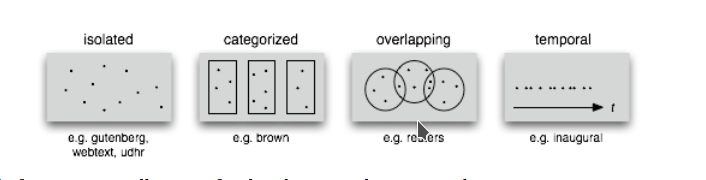
\includegraphics[width=.9\linewidth]{./assets/estructuras_de_corpus.png}
\caption{\label{fig:orgfb89153}Diferentes estructuras de corpus}
\end{figure}

\subsection{Analítica de datos}
\label{sec:orgdd24117}
La analítica de datos es una disciplina heterogenea que auna
diversas áreas de de estudio, como la teoría de la computación, la
estadística, los negocios y cualquier otro dominio sobre el cual es aplicada
(por ejemplo, química, biología, etc).  Una forma sucinta de
entender la analítica de datos es el proceso mediante el cual se
extrae \textbf{información} de los \textbf{datos} \cite{nelli2018python}. Así,
se entiende por dato un registro que representa una medida de
algún fenómeno observable. Por otro lado, la información se
entiende como el conjunto de conclusiones aplicables que se
obtienen de los datos luego de ser procesados. Tal proceso es
el que se conoce como \textbf{análisis de datos}. El análisis
de datos es variado y utiliza distintos recursos estadísticos
y matemáticos, pero por lo general la análitica de datos
tiene por objetivo generar un \emph{modelo} de los datos
que tenga capacidad \emph{predictiva}.

Como se ve, la análitica de datos provee, más que un resultado
concreto, una metodología para obtener modelos. Este trabajo,
por lo tanto, se enmarca dentro de la analítica de datos
en la medida en que se propone un modelo y lo evalua haciendo
uso de rasgos comunes como: el uso de repositorios de datos
(corpus), el uso de la estadística descriptiva para evaluar
el modelo, la formalización de un modelo en términos matemáticos
y el uso del stack de analítica de datos de Python (Pandas, Numpy,
Seaborn, ScikitLearn).

Ahora bien, si bien en este trabajo se enmarca dentro de la
analítica de datos, se debe aclarar que el modelo presentado
\textbf{no} es producido a partir de ninguna técnica  de Machine Learning.

En cuanto a la información específica de la metodología, este
proyecto se guió por la metodología CRIPS-DM

\subsection{CRISP-DM}
\label{sec:orgba74543}
El Cross Industry Standard Process for Data Mining (CRISP-DM) es
un modelo que sirve de base para cualquier proceso de analítica de
datos. Este consta de 6 fases: 1) Entendimiento del negocio (¿Qué
necesita el negocio?), 2) Entendimiento de los datos (¿Qué datos
tenemos/necesitamos?¿Se necesitan limpiar?), 3) Preparación de los
datos (¿Cómo organizamos los datos para modelar?), 4) Modelamiento
(¿Qué técnicas de modelamiento deberíamos aplicar?), 5) Evaluación
(¿El modelo cumple con los objetivos de negocio?) y 6) Despliegue
(¿Cómo acceden a los resultados los interesados?).

CRISP-DM se utiliza, por lo tanto, como una guía para
asegurar que cada fase del proceso de análitica de datos
tenga las consideraciones adecuadas. Así el Diseño Metodológico
de este trabajo está organizado según las fases mencionados.
Sin embargo, cabe aclarar que algunas modificaciones debieron
ser hechas a las fases, sobre todo a lo concerniente con las
fases de Evaluación y Despliegue, pues el objetivo de este
trabajo no es producir un modelo utilizado en un entorno empresarial.




\section{MARCO REFERENCIAL}
\label{sec:org35c4cce}

El trabajo de Delmonte \cite{delmonte2013computing} presenta a
SPARSAR, un sistema para calcular automáticamente el estilo de la
poesía. SPARSAR funciona sobre sistemas previos del mismo autor, como,
por ejemplo, un analizador semántico \cite{delmonte2005venses}.
Delmonte tiene una larga trayectoria en el modelamiento de conceptos
lingüísticos "difíciles", como la prosodia y la rima en términos
cuantitativos.

El aporte principal de Delmonte fue su innovación al momento de aplicar
herramientas comunes de NLP (tokenizadores, splitters y NER) con el fin
de analizar aspectos estilísticos de un texto. Los modelos de Delmonte
son muy cercanos a la teoría lingüística y propone soluciones a aspectos
complejos del análisis lingüístico. Esta proximidad me llevo a
plantearme la pregunta ¿qué otros aspectos del lenguaje valdría la pena
modelar que aún no hayan sido abordados desde una perspectiva
computacional? Así mismo, Delmonte reporta que hay pocos trabajos en el
área con este mismo enfoque. Esta fue una inspiración para explorar más
en el tema y ofrecer un enfoque distinto, tal como él lo hizo.

Sin embargo, Delmonte no revela detalles de implementación de sus sis-
temas en los artículos revisados. Además, sus sistemas tienen una
alcance mucho mayor que el dispuesto para este trabajo, por lo que para
mayores detalles tuve que referirme a otros trabajos.

El trabajo de \cite{zuniga2017automatic} establece una métrica para
medir el grado de creatividad en la poesía, basándose en qué tanto de
la rima se conserva en la traducción de un poema con respecto al
original. Tomé de Zuñiga la idea de establecer una métrica para un
aspecto tradicionalmente cualitativo (la creatividad). Lo que
diferencia este trabajo del de Delmonte, es su aproximación
matemática. Particularmente, Zuñiga ofreció una forma naive de
calcular similitud en rima, sin necesidad de recurrir a construcciones
que requieren de recursos léxicos complejos como una ontología para
fonemas, etc.

Por último, el trabajo de \cite{kaplan2006computational} es una tesis
de pregrado sobre el cálculo del estilo de la poesía desde una
perspectiva estadística. Kaplan fue una inspiración para Delmonte, por
lo tanto debía formar parte de la revisión bibliográfica. Kaplan
formuló un modelo que media 84 métricas distintas para cada documento,
luego transformó el modelo de 84 métricas para visualizarlo en un
espacio 3D y poder comparar distintas obras literarias. Esto inspiró
la idea inicial de obtener una métrica más general para analizar un
texto, que no tenga que recurrir un trabajo de compilación de métricas
existentes, como lo hizo Kaplan. Tal métrica debería estar sustentada
en conceptos linguísticos, para lo cual se recurrió a  los conceptos
presentados en el marco teórico.

\section{DISEÑO METODOLÓGICO}
\label{sec:orga4a6548}
El diseño metodológico seguirá --a grandes rasgos-- los pasos de la
metodología CRISP-DM, que se considera un estándar \emph{de facto} para
proyectos de minería de datos. Esta metodología ayudará organizar
el proceso de mi investigación, que vá desde el acceso a los corpus
(los datos disponibles) hasta el despliegue (la visualización de
los resultados).

\subsection{Entendimiento del negocio}
\label{sec:org8299494}

El resultado tangible del modelo de literariedad propuesto son dos
métricas cuantitativas: \emph{metáfora} y \emph{metonímia}.  Estas métricas
juntas constituiran una representación 'objetiva' del concepto
cualitativo de \emph{literariedad}.

\begin{figure}[htbp]
\centering
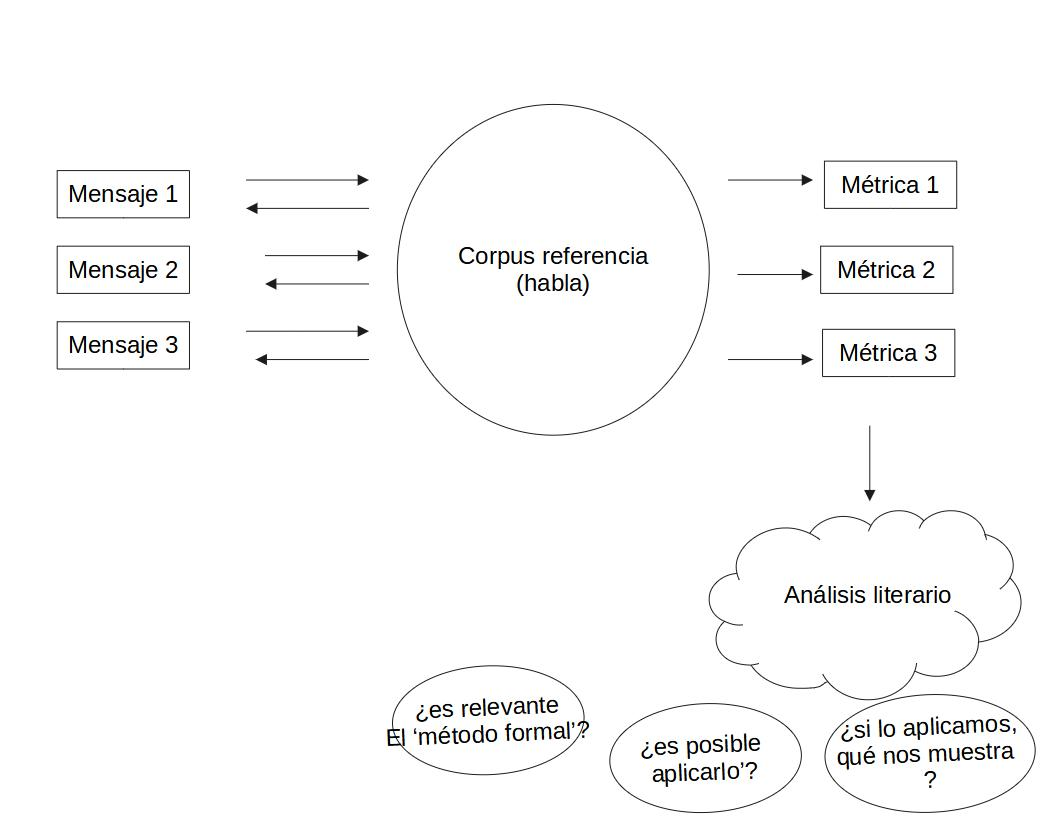
\includegraphics[width=.9\linewidth]{./assets/posibles_usos.jpg}
\caption{\label{fig:posibles_usos}Entradas y salidas del algoritmo}
\end{figure}


¿Cuál sería el beneficio de obtener este resultado? Se podría
comparar las métricas de n mensajes cualesquiera y tener una
medida objetiva con las cuales compararlas. Algunos casos de uso
posible serían:

\begin{itemize}
\item determinar si un mensaje que yo he escrito es más metáforico o
metonímico que otro.

\item determinar si un mensajes de una misma categoria (por ejemplo,
del mismo autor, o del mismo género) tienen medidas de métadora
y metonímia similares.

\item correr grandes grupos de mensajes, por ejemplo, 'poemas de la
escuela simbolistas' y compararlo con 'poemas realistas' y
verificar si hay o no una diferencia sustancial desde el punto
de vista linguístico .
\end{itemize}

Como se puede apreciar (ref:fig:posibles\textsubscript{usos}), las aplicaciones
del modelo en principio supondrían un factor adicional para ser
considerado para el estudio literario, cuya naturaleza es
cualitativa. Sin embargo, si el modelo demuestra ser efectivo,
podría llegar a ser una medida de similitud para un texto, lo que
implicaría que se podría clasificar un texto con base en su
metáfora y metonímia,


\subsection{Entendimiento de los datos}
\label{sec:org3e188ae}

En esta sección, se enumeraran las distintas fuentes de datos,
que en este caso vendrían a ser los diferentes tipos de corpus.


\subsubsection{El corpus de referencia}
\label{sec:org10a131a}

El corpus de referencia es un compendio de muestras
que terminará por representar un consenso sobre
el uso de la \emph{lengua}. Su correlación teórica
es el eje de diacronía y cumple la función de
cristalizar una lengua en un lugar y un tiempo establecido.
A nivel de implementación, se trata de un cadena muy larga
compuesto de muestras seleccionadas según criterios aptos
(ver sección sobre preparación de los datos).




\subsubsection{El corpus objetivo}
\label{sec:orgf25fa24}

El corpus objetivo serán los mensajes sobre los cuales se
computarán las dos medidas de \emph{metáfora} y \emph{metonimia}.
Su correlativo teórico es el \emph{habla} y son los
textos que el usuario final del final del sistema desea
someter a análisis. A nivel de implementación, cada mensaje
es una cadena (que corresponde a un documento real), pero
en su totalidad el corpus objetivo es mucho más pequeño
que el corpus de referencia, del mismo modo en que una
persona que profiere una oración utiliza un subconjunto
mucho más pequeño de la lengua a la que pertenece.  

\subsubsection{La red semántica}
\label{sec:org25515d8}

La red semántica es un tipo de corpus particular que no solamente
consta de palabras anotadas, como el de Brown, sino que vincula
las palabras por su relación conceptual con otras palabras. La
red semántica correspondería a la facultad de asociar conceptos
con las "imágenes acústicas" (las palabras) de Saussure. En esta
investigación, la red semántica se utilizará para obtener
sínonimos de palabras, que representarán conceptos. Tal red
no será implementada, sino que será un servicio utilizado por
el algoritmo. 



\subsubsection{Resumen de entendimiento de los datos}
\label{sec:org8523e0b}
\begin{figure}[htbp]
\centering
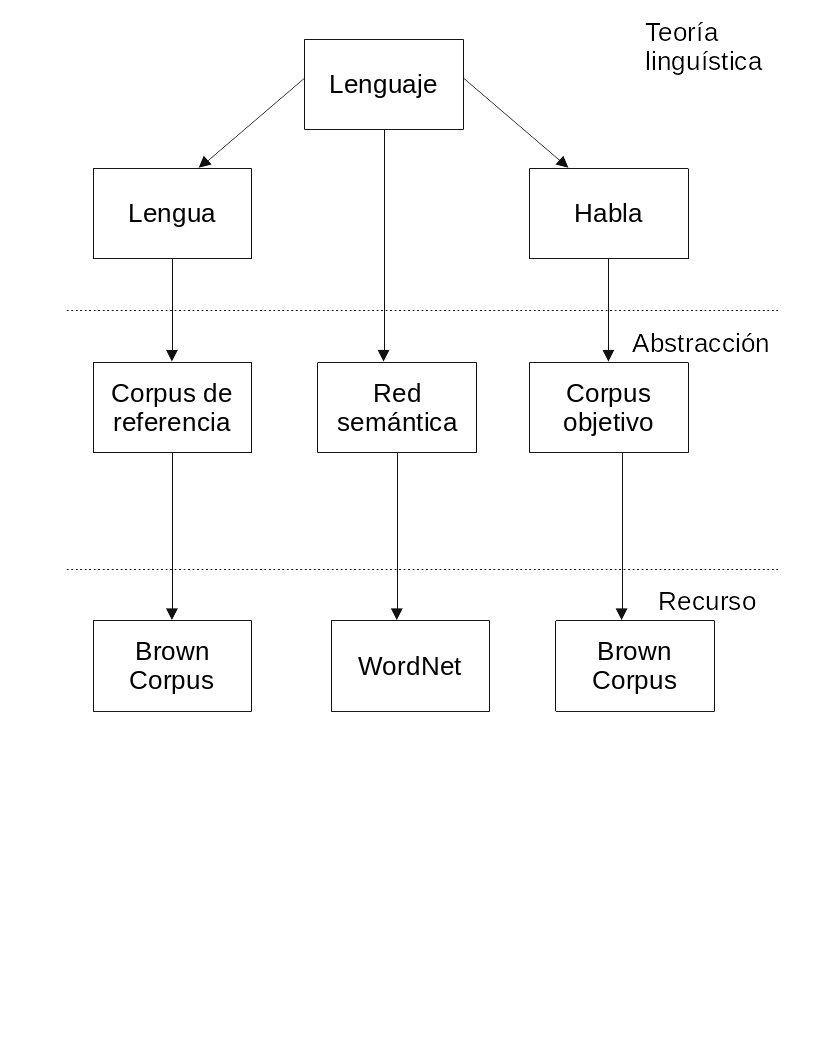
\includegraphics[width=.9\linewidth]{./assets/entendimiento_de_los_datos.png}
\caption{Resumen de las fuentes de datos utilizadas para cada concepto}
\end{figure}


\subsection{Preparación de los datos}
\label{sec:orgad93403}
\label{sec:preparacion_datos}
La tarea de preparación de los datos consitirá principalmente en
seleccionar los distintos tipos de corpus de manera significativa
y coherente.  A continuación, describiré cómo se conformaron los
corpus y qué criterios se utilizaron.

\subsubsection{Corpus de referencia}
\label{sec:orgaacf8d7}

El corpus de referencia representa la \emph{lengua} (\emph{langue}). Por lo
tanto debe estar compuesto de una muestra de textos
comparativamente mucho más grande los mensajes individuales que
serán contrastados con este. ¿Cómo construir un corpus tal?

En primer lugar, se descartó la idea de modelar la \emph{lengua} en su
totalidad, pues como lo indica la teoría linguística, esta tarea
es imposible puesto que esta se encuentra en constante
cambio. Así, el primer criterio para construcción del corpus fue
restringirlo diacrónicamente al espacio de un año y a un idioma
específico.

El siguiente criterio fue armar un corpus \emph{balanceado}. Es decir,
el corpus de referencia no puede estar compuesto de muestras de
un mismo tipo (un estilo, un género, un autor), porque esto
sesgaría la comparación de el corpus objetivo con respecto a
este. Así, se optó por partir de un corpus \emph{categorizado} y tomar
partes iguales de cada una de las categorias. Esto es, cada
categoría tiene igual peso en cuanto a número de textos y
palabras que lo representan.

El tercer criterio fue utilizar un corpus fácilmente accesible,
de origen libre y avalado por la comunidad científica. Por todos
los motivos anteriores, se escogió el corpus de Brown, que
presenta las siguientes características:

\begin{itemize}
\item todas las muestras del corpus pertenecen al año 1961
\item todas las muestras del corpus se imprimieron en Estados Unidos durante ese año
\item todos los autores son hablantes nativos de inglés
\item la categorización de las muestras fue hecha por un comité de expertos de la universidad de Brown
\item la intención declarada del corpus es la de ser una muestra representativa del inglés de aquel año
\item tiene una lista amplia de categorías que podrían ser útiles para observar diferencias entre las categorías
\item los resultados obtenidos del modelo podrían ser replicados porque el corpus es ampliamente conocido
\end{itemize}

En la tabla \ref{tab:corpus_referencia} se muestra lo que se
utilizará como corpus de referencia.



    \begin{longtable}{| p{.20\textwidth} | p{.40\textwidth} | p{.20\textwidth}|} 
    \hline
        cód.  & nombre  & categoria  \\ \hline
        a01 & Political Reportage & reportage  \\ \hline
        a11 & Sports Reportage & reportage  \\ \hline
        a19 & Spot News & reportage  \\ \hline
        a26 & Financial Reportage & reportage  \\ \hline
        a40 & People, Art \& Education & reportage \\ \hline
        b03 & Editorials & editorial  \\ \hline
        b08 & Columns & editorial  \\ \hline
        b15 & Letters to the editor & editorial  \\ \hline
        b19 & The Voice of the people & editorial \\ \hline
        b24 & Reviews & editorial \\ \hline
        d15 & Zen:A Rational critique & religion  \\ \hline
        d11 & War \& the Cristian Conscience & religion  \\ \hline
        d13 & The New Science \& The New Faith & religion  \\ \hline
        d04 & The Shape of death & religion  \\ \hline
        d02 & Christ Without Myth & religion  \\ \hline
        e05 & The Younger Generation/Use of Common Sense Makes Dogs Acceptable & skills \& hobbies \\ \hline
        e06 & The American Boating Scene & skills \& hobbies  \\ \hline
        e10 & The New Guns of 61 & skills \& hobbies  \\ \hline
        e19 & How to Own a Pool and Like It & skills \& hobbies  \\ \hline
        e23 & The Watercolor Art or Roy Mason & skills \& hobbies  \\ \hline
        f07 & How to Have a Successful Honeymoon/Attitudes Toward Nudity & popular lore  \\ \hline
        f12 & New Methods of Parapsychology & popular lore  \\ \hline
        f13 & Part-time Farming & popular lore  \\ \hline
        f14 & The Trial and Eichmann & popular lore  \\ \hline
        f33 & Slurs and Suburbs & popular lore  \\ \hline
        g15 & Themes and Methods: Early Storie of Thomas Mann & belles lettres  \\ \hline
        g13 & Sex in Contemporary Literature & belles lettres  \\ \hline
        g18 & Verner von Heidenstam & belles lettres  \\ \hline
        g26 & Two Modern Incest Heroes & belles lettres  \\ \hline
        g28 & William Faulkner, Southern Novelist & belles lettres \\ \hline
        j18 & Linear Algebra & learned  \\ \hline
        j17 & Prolegomena to a Theory of Emotions & learned  \\ \hline
        j28 & Perceptual Changes in Psycopathology & learned  \\ \hline
        j39 & Stock, Wheats and Pharaohs & learned \\ \hline
        j35 & Semantic Contribution of Lexicostatistics & learned  \\ \hline
        k18 & Midcentaury & general fiction  \\ \hline
        k25 & The Prophecy & general fiction  \\ \hline
        k04 & Worlds of Color & general fiction  \\ \hline
        k23 & The Tight of the Sea & general fiction  \\ \hline
        k17 & Mila 8 & general fiction  \\ \hline
        l05 & Bloodstain & mistery and detective fiction  \\ \hline
        l11 & The Man Who Looked Death in the Eye & mistery and detective fiction  \\ \hline
        l04 & Encounter with Evil & mistery and detective fiction  \\ \hline
        l19 & Make a Killing & mistery and detective fiction  \\ \hline
        l20 & Death by the Numbers & mistery and detective fiction  \\ \hline
        m01 & Stranger in a Strange Land & science fiction  \\ \hline
        m03 & The Star Dwellers & science fiction  \\ \hline
        m04 & The Planet with no Nightmare & science fiction  \\ \hline
        m05 & The Ship who Sang & science fiction  \\ \hline
        m06 & A Planet Named Shayol & science fiction  \\ \hline
        n01 & The Killer Marshall & adventure and western fiction  \\ \hline
        n05 & Bitter Valley & adventure and western fiction  \\ \hline
        n15 & Sweeny Squadron & adventure and western fiction  \\ \hline
        n20 & The Flooded Deares & adventure and western fiction  \\ \hline
        n26 & Toughest Lawman in the Old West & adventure and western fiction  \\ \hline
        p29 & My Hero & romance and love story  \\ \hline
        p27 & Measure of a Man & romance and love story  \\ \hline
        p22 & A Husband Stealer from Way Back & romance and love story  \\ \hline
        p16 & A Secret Between Friends & romance and love story  \\ \hline
        p12 & A Passion in Rome & romance and love story  \\ \hline

  \caption{Corpus de referencia}
\label{tab:corpus_referencia}
\end{longtable}

\subsubsection{Corpus objetivo}
\label{sec:orgb4bb994}
En contrapartida al corpus de referencia, el corpus objetivo representa el
\emph{habla} (\emph{parole}). Así, estos son considerados mensajes que serán interpretados
por el receptor con relación al consenso de la lengua compartida entre emisor y
receptor.

El primer criterio para construir el corpus de referencia es que este tenga
una delimitacion diacrónica igual a la de el corpus objetivo. El segundo
criterio, que las categorías fueran comparables a las categorias establecidas
del corpus de referencia.

El tercer criterio es que cada muestra del corpus del corpus objetivo
tuviera un tamaño similar entre sí, para descartar que diferencias
en la longitud del mensaje afectaran sustancialmente los resultados del algoritmo

Por estos motivos, se optó por tomar tomar muestras del mismo corpus de Brown.
La diferencia radica en que cada categoría solo tiene una muestra y la muestra
seleccionada para la categoría está ausente en el corpus objetivo. Así,
el corpus objetivo presenta las siguientes características:

\begin{itemize}
\item es una muestra 'miniatura' del corpus de Brown
\item la relación de tamaño entre el corpus objetivo y el corpus de Brown es de 1:5
\item Cada categoría en el cropus objetivo tiene su correlativo en el de referencia y viceversa
\item el tamaño de cada muestra es de cerca de 2000 palabras
\end{itemize}

A continuación, se presenta un resumen del corpus objetivo en las
tablas \ref{tab:corpus_objetivo1},
\ref{tab:corpus_objetivo2}, \ref{tab:corpus_objetivo3},
\ref{tab:corpus_objetivo4} y \ref{tab:corpus_objetivo5}.



   \begin{table}[!ht]
    \centering

    \begin{tabular}{|l|l|l|}
    \hline
	cód & nombre & categoría \\ \hline
      a40 & People. Art \& Education & reportage \\ \hline
      b27 & Letters to the Editor & editorial \\ \hline
      c17 & Reviews & reviews \\ \hline
      d09 & Organizing the Local Church & religion \\ \hline
      e36 & Renting a Car in Europe & skills \& hobbies \\ \hline
      f48 & Christian Ethics \& the Sit-In & popular lore \\ \hline
      g75 & A Wreath for Garibaldi & belles lettres \\ \hline
      h30 & Annual Report of Year Ending June 30:1961 & miscellaneous \\ \hline
      j80 & Principles of Inertial Navigation & learned \\ \hline
      k29 & The Sheep's in the Meadow & general fiction \\ \hline
      l24 & The Murders & mistery and detective fiction \\ \hline
      m02 & The Lovers & science fiction \\ \hline
      n29 & Riding the Dark Train Out & adventure and western fiction \\ \hline
      p20 & Dirty Dig Inn & romance and love story \\ \hline
    \end{tabular}
\caption{Corpus objetivo 1}
\label{tab:corpus_objetivo1}
\end{table}




     \begin{table}[!ht]
      \centering
      \begin{tabular}{|l|l|l|}
      \hline
cód & nombre & categoría \\ \hline
        a02 & The Dallas Morning News & reportage \\ \hline
        b01 & The Atlanta Constitution & editorial \\ \hline
        c01 & Chicago Daily Tribune & reviews \\ \hline
        d01 & William G. Pollard Physicist and Christian & religion \\ \hline
        e02 & Organic Gardening and Farming & skills \& hobbies \\ \hline
        f01 & How Much Do You Tell When You Talk? & popular lore \\ \hline
        g01 & Northern Liberals and Southern Bourbons & belles lettres \\ \hline
        h01 & Handbook of Federal Aids to Communities & miscellaneous \\ \hline
        j01 & Radio Emission of the Moon and Planet & learned \\ \hline
        k01 & First Family. & general fiction \\ \hline
        l02 & Bachelors Get Lonely & mistery and detective fiction \\ \hline
        m01 & Stranger in a Strange Land & science fiction \\ \hline
        n02 & The Valley & adventure and western fiction \\ \hline
        p01 & A Cup of the Sun & romance and love story \\ \hline
      \end{tabular}
  \caption{Corpus objetivo 2}
  \label{tab:corpus_objetivo2}
  \end{table}


\begin{table}[!ht]
 \centering

 \begin{tabular}{|l|l|l|}
 \hline
cód & nombre & categoría \\ \hline
        a03 & Chicago Daily Tribune & reportage \\ \hline
        b02 & The Christian Science Monitor & editorial \\ \hline
        c02 & The Christian Science Monitor & reviews \\ \hline
        d03 & Christian Unity in England & religion \\ \hline
        e03 & Will Aircraft or Missiles Win Wars? & skills \& hobbies \\ \hline
        f02 & America's Secret Poison Gas Tragedy & popular lore \\ \hline
        g02 & Toward a Concept of National Responsibility & belles lettres \\ \hline
        h02 & An Act for International Development & miscellaneous \\ \hline
        j02 & Proceedings of the 1961 Heat & learned \\ \hline
        k02 & The Ikon & general fiction \\ \hline
        l03 & Encounter with Evil & mistery and detective fiction \\ \hline
        m03 & The Star Dwellers & science fiction \\ \hline
        n03 & Trail of the Tattered Star & adventure and western fiction \\ \hline
        p02 & Seize a Nettle & romance and love story \\ \hline
      \end{tabular}
  \caption{Corpus objetivo 3}
  \label{tab:corpus_objetivo3}
  \end{table}


   \begin{table}[!ht]
      \centering
 \begin{tabular}{|l|l|l|}
 \hline
cód & nombre & categoría \\ \hline
        a04 & The Christian Science Monitor & reportage \\ \hline
        b04 & The Miami Herald:September & editorial \\ \hline
        c03 & The New York Times & reviews \\ \hline
        d05 & Theodore Parker: Apostasy within Liberalism & religion \\ \hline
        e04 & High Fidelity & skills \& hobbies \\ \hline
        f03 & I've Been Here before! & popular lore \\ \hline
        g03 & The Chances of Accidental War & belles lettres \\ \hline
        h03 & 87th Congress: 1st Session. House Document No. 247. & miscellaneous \\ \hline
        j03 & The Normal Forces and Their Thermodynamic Significance & learned \\ \hline
        k03 & Not to the Swift & general fiction \\ \hline
        l06 & Hunter at Large & mistery and detective fiction \\ \hline
        m04 & The Planet with No Nightmare & science fiction \\ \hline
        n04 & The Shadow Catcher & adventure and western fiction \\ \hline
        p03 & The Fairbrothers & romance and love story \\ \hline
     
      

      \end{tabular}
  \caption{Corpus objetivo 4}
  \label{tab:corpus_objetivo4}
  \end{table}


      \begin{table}[!ht]
    \centering

    \begin{tabular}{|l|l|l|}
    \hline
      cód & nombre & categoría \\ \hline
      a05 & The Providence Journal & reportage \\ \hline
      b05 & Newark Evening News & editorial \\ \hline
      c04 & The Providence Journal & reviews \\ \hline
      d06 & Tracts published by American Tract Society & religion \\ \hline
      e07 & How to design your Interlocking Frame & skills \& hobbies \\ \hline
      f04 & North Country School Cares for the Whole Child & popular lore \\ \hline
      g04 & The Invisible Aborigine & belles lettres \\ \hline
      h04 & Rhode Island Legislative Council & miscellaneous \\ \hline
      j04 & Proton magnetic resonance study & learned \\ \hline
      k05 & The Judges of the Secret Court & general fiction \\ \hline
      l07 & Deadlier Than the Male. & mistery and detective fiction \\ \hline
      m05 & The Ship Who Sang & science fiction \\ \hline
      n06 & Here Comes Pete Now. & adventure and western fiction \\ \hline
      p04 & The Moon and the Thorn. & romance and love story \\ \hline

    \end{tabular}
\caption{Corpus objetivo 5}
\label{tab:corpus_objetivo5}
\end{table}
\subsection{Modelamiento}
\label{sec:org28a909c}
\subsubsection{Selección de técnica de modelado}
\label{sec:orgcbcf678}

Esta investigación se enmarca dentro de un enfoque mixto, en
donde se utilizan métodos tanto cualitativos (el marco teórico) como
cuantitativos, por lo tanto, hay varias técnicas implicadas  en el modelado.

Desde el aspecto cuantitativo, se utilizan técnicas conocidas
dentro del NLP, como tokenizacion, n-gramas y  bag-of-words.
Estas técnicas se utilizan como medios de vectorización, mediante
lo cual se logra un transformación de un texto (una variable cuantitativa)
a una representación númerica, (la matriz de uso).

Desde el aspecto cualitativo, se hizo una revisión de la literatura y de la intuición
para acotar los planteamientos de la teoría, los conceptos de \emph{lengua} y \emph{habla}, hasta
una formulación cuantificable con los métodos descritos.




\subsubsection{Diseño experimental}
\label{sec:org432493c}

Una vez formulado el modelo, se conduce un experimento que evaluará si produce resultados
satisfactorios. El objetivo del experimento es escudriñar si los valores arrojados para
los índices propuestos son coherentes con las intuiciones detrás del marco teórico y/o
con el 'juicio experto'.

El experimento se basa en una cualidad del corpus de referencia seleccionado: su categorización.
Por lo tanto, como se explica en la sección \ref{sec:preparacion_datos}, se seleccionaron
muestras del Corpus de Brown  de tal modo que cada categoría está representada igualmente
en cada muestra. Así, luego de procesar las muestras, se compararán los resultados por
cada categoría.

El modelo se considerará existoso si los valores del índice metafórico e índice metonímico
son consistentes a lo largo de las muestras para cada categoría.

Además, dentro de cada muestra, se espera que se cumplan ciertas hipótesis:

\begin{itemize}
\item H1: Se espera que las categorías de ficción tengan un índice metafórico significativamente mayor que los de no-ficción
\item H2: Se espera que las categorias 'Reportage' y 'Editorial' tengan índices metafóricos similares a través de las muestras
\item H3: Se espera que la categoría 'Belles Lettres' tenga un indíce metafórico más alta entre las categorías de no-ficción
\item H4: Se espera que la categoria 'Learned' tenga un indice metonímico bajo en general
\end{itemize}


No se formularán más hipotesis acerca del índice metonímico, pues según los planteamientos teóricos este indicador
es sensible especialmente al género de poesía, que no está presente en la muestra por las limitaciones del corpus
seleccionado.



\subsubsection{Presentación del modelo}
\label{sec:org002dd7e}
El modelo diseñado se basa en las siguientes ecuaciones. Para una visión a más alto nivel del
procedimiento se puede ver la figura \ref{fig:metodologia}

      \begin{equation}\label{eq:mensaje}
mensaje = \{ w_1, w_2, w_3, \dots , w_j \} \\
\end{equation}

\begin{equation}\label{eq:vector_semantico}
vector\ semantico(w) = \{s_1, s_2, s_3, \dots, s_j \} \\
\end{equation}

\begin{equation}\label{eq:vector_uso}
vector\ uso(w) = \{freq(s_1),freq(s_2),freq(s_3), \dots, freq(s_j) \} \\
\end{equation}

\begin{equation}\label{eq:uso}
uso(w) = \frac{\mu (vector\ uso)}{freq(w)}
\end{equation}


\begin{equation}\label{eq:indice_metafórico}
indice\ metaforico(mensaje) =  \Sigma_i^j \frac{uso(w_i)}{\mu( vector\ semantico(w_i))}
\end{equation}


\begin{equation}\label{eq:ngramas}
N = \{n_1, n_2, n_3, \dots , n_j\}
\end{equation}

\begin{equation}\label{eq:metonimia}
met(n) = \frac{letras\ iguales}{ set(letras(n_i1) + letras(n_i2)}
\end{equation}

\begin{equation}\label{eq:indice_metonimia}
indice\ metonimia = \Sigma_i^j met(n_i)
\end{equation}


En primer lugar, un mensaje es cualquier cadena de texto. Una vez
tokenizado, se obtienen las palabras  \(w\) mostradas en
la ecuación \ref{eq:mensaje}. Luego, para cada una de las palabras, se hace
primero el cálculo del vector semántico. Un vector semantico está
compuesto de sinónimos \(s\) del la palabra inicial (ecuación \ref{eq:vector_semantico}). Cuando se
termina de obtener los campos semánticos de cada palabra del mensaje,
se obtiene una matriz semántica. Luego, por cada vector semantico, se
calcula un vector de uso que cuenta la frecuencia de cada componente
del vector semantico \(s\) en el corpus de referencia \ref{eq:vector_uso}. La suma de
todos los vectores de uso de un mensaje se conoce como la matriz de
uso. Se puede apreciar las relación de las matrices semántica y de uso con
entre sí en la figura \ref{fig:matrices}.

Seguidamente, para cada vector de uso se calcula el uso, que es
la relación entre la media del vector de uso y la frecuencia de la
palabra en el corpus objetivo (ecuación \ref{eq:uso}). Así, si la palabra se utiliza más veces
que la media del vector de uso, se considera que la palabra está
siendo utilizada de manera más rara (más frecuente que lo indicaría
que se debe usar por su vector de uso), por ende el resultado del
cociente es mas alto y su aporte al índice metaforico mayor. El índice
metafórico es la suma de todos los usos, por lo que el índice en principio
solo captura si un mensaje es mas 'metafórico' que otro si tiene un número más alto
que otro mensaje y manteniendo lo longitud del mensaje.


Ahora, con respecto al Índice metonímico, se parte de la idea de que
un mensaje está compuesto de ngramas \(n\) (ver ecuación \ref{eq:ngramas}. Los ngramas son de nivel 2,
es decir, que se toman pares de palabras constiguas (ver figura \ref{fig:metonimia}) .
Luego para cada \(n\) se calcula la metonimia. La metonimia está dado por el numero de letras similares
entre los terminos \(n\) del bigrama \ref{eq:metonimia}. Por último, el Índice metonímico está dado
por la suma de la metonimima para cada ngrama. 



\begin{figure}[!H]
\centering
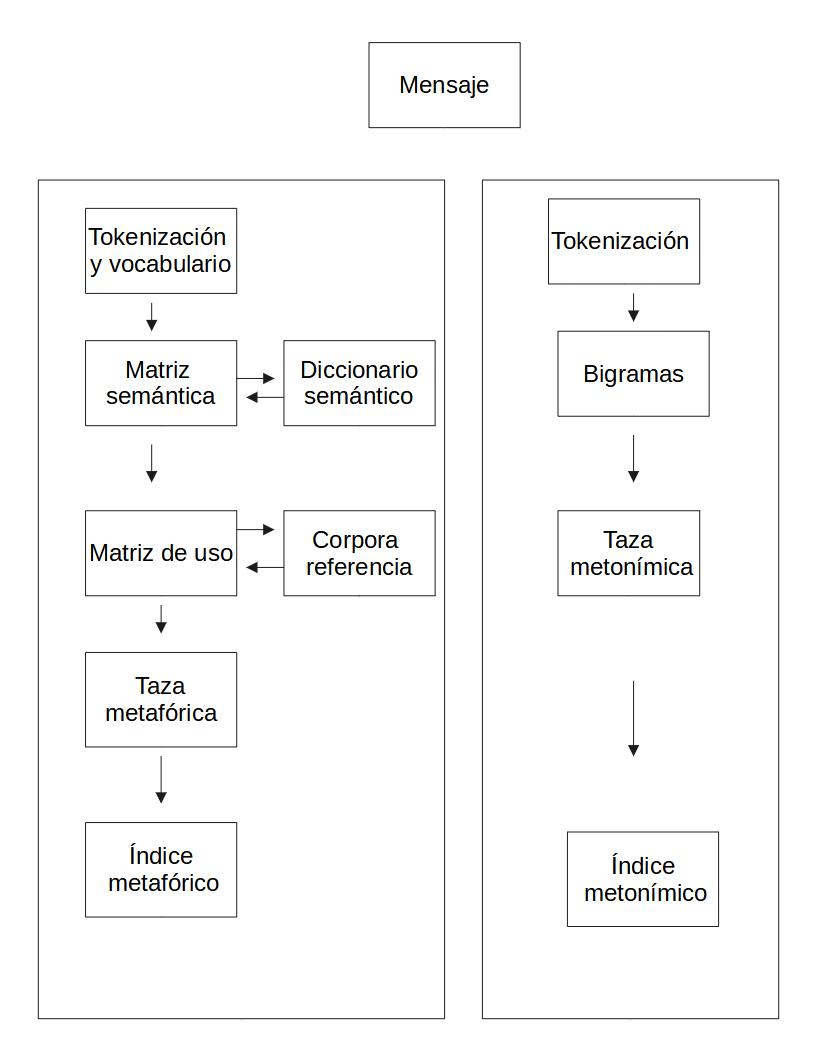
\includegraphics[width=0.7\textwidth]{./assets/metodologia.jpg}
\caption{\label{fig:metodologia}Metodología}
\end{figure}

\begin{enumerate}
\item Matrices de semántica y de uso
\label{sec:org56aa1a6}

\begin{figure}[!H]
\centering
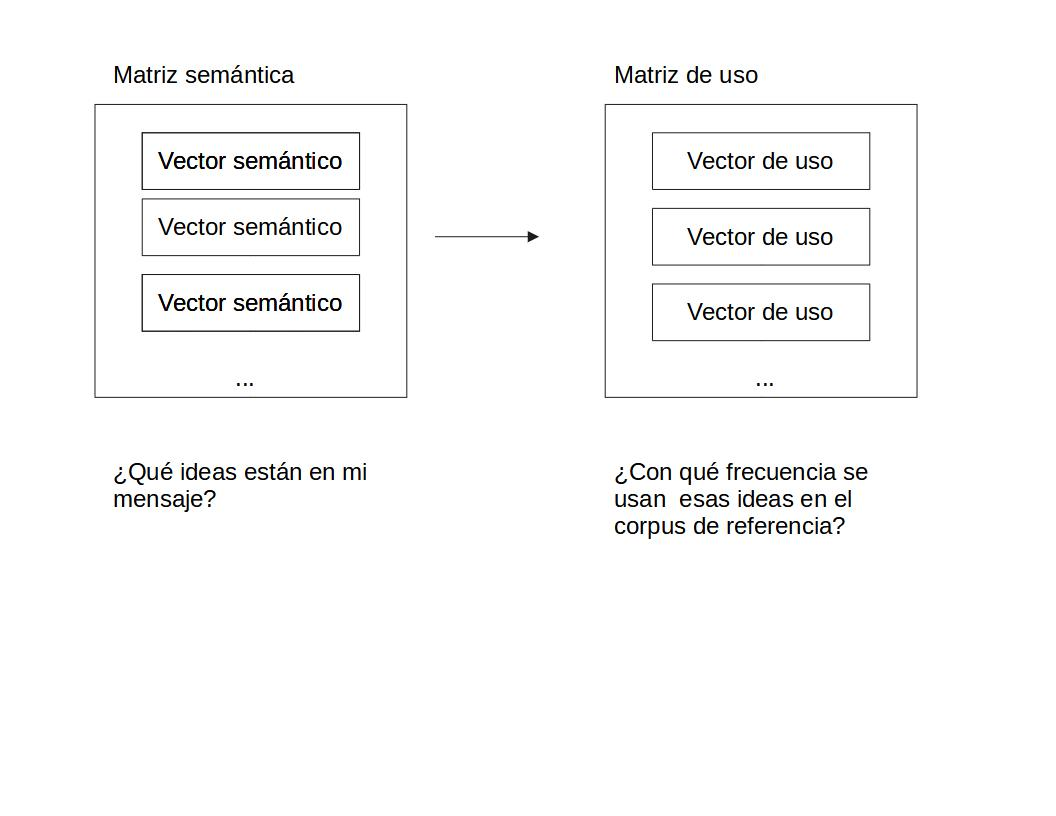
\includegraphics[width=0.7\textwidth]{./assets/matrices.jpg}
\caption{\label{fig:matrices}Abstracciones necesarias para el índice metafórico}
\end{figure}
\item Índice Metonímico
\label{sec:orgb9a0d9c}

\begin{figure}[!H]
\centering
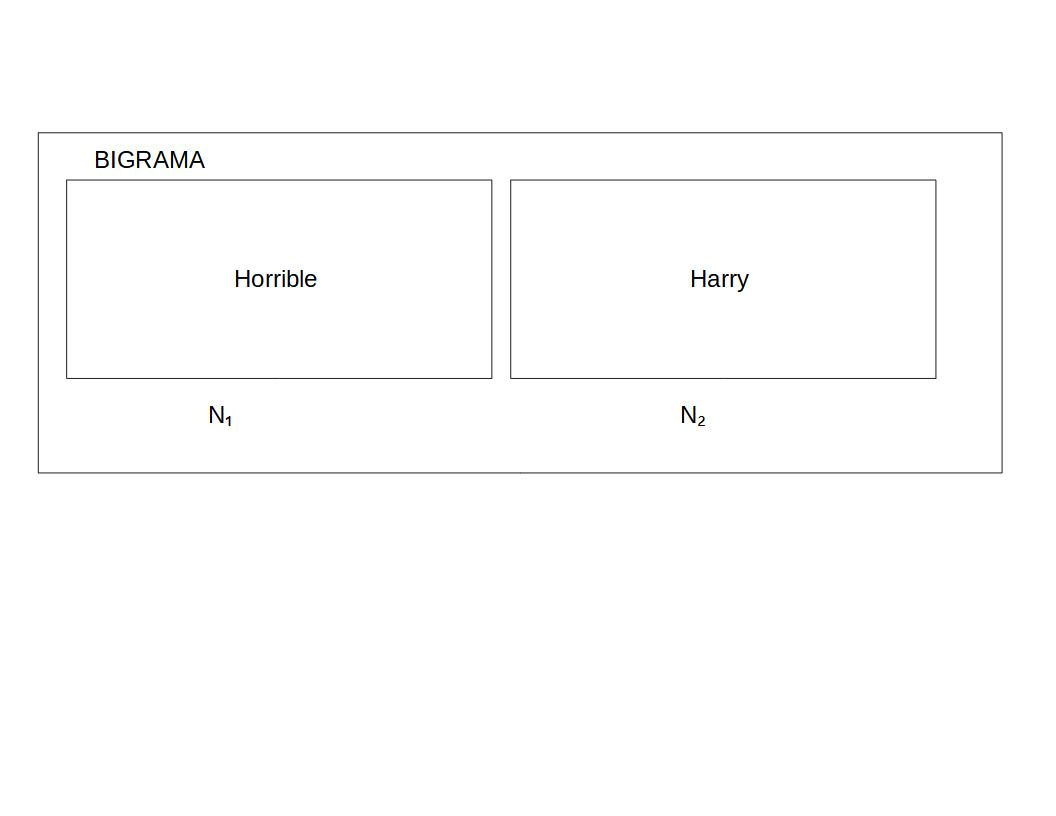
\includegraphics[width=0.7\textwidth]{./assets/metonimia.jpg}
\caption{\label{fig:metonimia}Concepto de metonimia}
\end{figure}
\end{enumerate}
\subsection{Despliegue}
\label{sec:orge8f4580}

\subsubsection{Índices por muestra}
\label{sec:org4ea5a78}

\begin{center}
    \begin{longtable}{| p{.20\textwidth} | p{.25\textwidth} | p{.25\textwidth}|p{.10\textwidth}|}
    \caption{Muestra 1}
    \hline
        categoria & metafora & metonimia & w \\ \hline
        reportage & 880514.226605173 & 232.266917233093 & 2340 \\ \hline
        editorial & 880324.393897166 & 245.719531857031 & 2262 \\ \hline
        reviews & 929802.38416219 & 242.953762332438 & 2370 \\ \hline
        religion & 850127.6846531 & 264.683072130827 & 2314 \\ \hline
        skills \& hobbies & 831781.725628903 & 242.632252469752 & 2232 \\ \hline
        popular lore & 833825.825225262 & 265.83988095238 & 2222 \\ \hline
        belles lettres & 877690.52541314 & 229.785869685869 & 2288 \\ \hline
        miscellaneous & 782613.273615479 & 278.192915417915 & 2214 \\ \hline
        learned & 863208.047211933 & 266.998263827676 & 2254 \\ \hline
        general fiction & 891211.57527208 & 249.95016095016 & 2264 \\ \hline
        mistery and detective fiction & 1032943.85669407 & 244.615023865023 & 2446 \\ \hline
        science fiction & 1064426.54657215 & 235.067805233981 & 2412 \\ \hline
        adventure and western fiction & 1234204.19460692 & 229.817769158945 & 2560 \\ \hline
        romance and love story & 993413.094671098 & 217.506968031968 & 2428 \\ \hline
\end{longtable}
\label{muestra1}
\end{center}

\begin{center}
    \begin{longtable}{| p{.20\textwidth} | p{.25\textwidth} | p{.25\textwidth}|p{.10\textwidth}|}
\caption{Muestra 2} 
    \hline
         categoria & metafora & metonimia & w \\ \hline
        reportage & 869205.2371696023 & 233.99592490842463 & 2277 \\ \hline
        editorial & 777241.5394134748 & 252.29809496059465 & 2200 \\ \hline
        reviews & 978095.225396233 & 242.3226565101564 & 2415 \\ \hline
        religion & 831466.3628116096 & 234.21091131091077 & 2213 \\ \hline
        skills \& hobbies & 833209.3790445685 & 237.43338605838585 & 2279 \\ \hline
        popular lore & 965391.1906183016 & 270.5444999444997 & 2369 \\ \hline
        belles lettres & 863139.7507327744 & 279.74454989454966 & 2289 \\ \hline
        miscellaneous & 873426.7117151126 & 302.2738428238428 & 2416 \\ \hline
        learned & 912477.0323082526 & 241.59998334998312 & 2189 \\ \hline
        general fiction & 1025249.8452137534 & 243.0625180375174 & 2440 \\ \hline
        mistery and detective fiction & 959584.2017381956 & 231.74134476634435 & 2370 \\ \hline
        science fiction & 1049847.7175834612 & 260.93059440559404 & 2486 \\ \hline
        adventure and western fiction & 1079790.9124281127 & 232.90989288489175 & 2383 \\ \hline
        romance and love story & 969075.2121776282 & 261.1946331446324 & 2332 \\ \hline
    \end{longtable}
    \label{muestra2}
\end{center}


\begin{center}
        \begin{longtable}{| p{.2\textwidth} | p{.25\textwidth} | p{.25\textwidth}|p{.10\textwidth}|}
\caption{Muestra 3}
    \hline
          categoria & metafora & metonimia & w \\ \hline
        reportage & 832961.122494042 & 253.461402486402 & 2275 \\ \hline
        editorial & 798751.012651529 & 266.66209346209246 & 2234 \\ \hline
        reviews & 884194.0844699917 & 249.01867299367268 & 2320 \\ \hline
        religion & 831865.8440237658 & 266.0598665223664 & 2332 \\ \hline
        skills \& hobbies & 850383.4965037219 & 263.1010350760349 & 2257 \\ \hline
        popular lore & 869221.9181097293 & 245.8761655011648 & 2264 \\ \hline
        belles lettres & 871094.3935751553 & 275.37426046176046 & 2311 \\ \hline
        miscellaneous & 839155.9869742717 & 295.0817980222388 & 2360 \\ \hline
        learned & 781733.2618728676 & 246.0817654567651 & 2182 \\ \hline
        general fiction & 924678.68595826 & 258.49646187146146 & 2325 \\ \hline
        mistery and detective fiction & 1123420.1486319497 & 259.7061299811289 & 2428 \\ \hline
        science fiction & 935994.4646234306 & 248.55044955044897 & 2364 \\ \hline
        adventure and western fiction & 1032713.1638679344 & 250.64708347208267 & 2380 \\ \hline
        romance and love story & 997559.1771764176 & 251.74584582084492 & 2320 \\ \hline
\end{longtable}
    \label{muestra3}
\end{center}

\begin{center}
\begin{longtable}{| p{.20\textwidth} | p{.25\textwidth} | p{.25\textwidth}|p{.10\textwidth}|}
\caption{Muestra 4}
    \hline
        categoria & metafora & metonimia & w \\ \hline
        reportage & 739005.545665808 & 273.2918525918524 & 2217 \\ \hline
        editorial & 839392.6586708553 & 252.962795537795 & 2230 \\ \hline
        reviews & 897166.8448193009 & 267.3208680208676 & 2356 \\ \hline
        religion & 971902.397216239 & 265.22606282606193 & 2410 \\ \hline
        skills \& hobbies & 913636.3833983988 & 260.77830780330754 & 2295 \\ \hline
        popular lore & 827298.639753781 & 263.91099178599177 & 2256 \\ \hline
        belles lettres & 948168.5408124946 & 263.5388195138189 & 2403 \\ \hline
        miscellaneous & 863483.173212439 & 246.39977799977743 & 2207 \\ \hline
        learned & 842569.1577530246 & 231.37843986079253 & 2205 \\ \hline
        general fiction & 917557.8900258496 & 230.44950882450823 & 2296 \\ \hline
        mistery and detective fiction & 866731.5026959036 & 245.56009546009463 & 2288 \\ \hline
        science fiction & 1102841.6209263606 & 248.0798007548002 & 2461 \\ \hline
        adventure and western fiction & 976789.2077744814 & 253.20416527916453 & 2349 \\ \hline
        romance and love story & 1111028.8409040042 & 248.49708902208823 & 2422 \\ \hline


\end{longtable}
    \label{muestra4}
\end{center}

\begin{center}
\begin{longtable}{| p{.20\textwidth} | p{.25\textwidth} | p{.25\textwidth}|p{.10\textwidth}|}
\caption{Muestra 5}
    \hline
        categoria & metafora & metonimia & w \\ \hline
        reportage & 804307.8590497638 & 254.57564380064355 & 2244 \\ \hline
        editorial & 797847.982604727 & 256.40300255300195 & 2241 \\ \hline
        reviews & 926295.4083615864 & 234.46358363858295 & 2342 \\ \hline
        religion & 935931.8321572712 & 233.24144189144172 & 2317 \\ \hline
        skills \& hobbies & 916884.62774593 & 232.22511377511276 & 2370 \\ \hline
        popular lore & 796816.1152101667 & 263.7263361638353 & 2258 \\ \hline
        belles lettres & 861343.6692835388 & 239.3655889861766 & 2359 \\ \hline
        miscellaneous & 863173.038736266 & 279.4144463379755 & 2316 \\ \hline
        learned & 907069.3580927892 & 255.3453282828281 & 2334 \\ \hline
        general fiction & 870179.8901159727 & 224.0298867798861 & 2345 \\ \hline
        mistery and detective fiction & 914219.7991227966 & 256.1841630591622 & 2331 \\ \hline
        science fiction & 1000556.046812526 & 255.7852647352645 & 2369 \\ \hline
        adventure and western fiction & 835693.3281863902 & 228.3971750471748 & 2279 \\ \hline
        romance and love story & 1113220.902539808 & 261.2546370296359 & 2546 \\ \hline
\end{longtable}
    \label{muestra5}
\end{center}
\subsubsection{Gráficos por muestra}
\label{sec:orgadccf66}

\begin{figure}[!htbp]
\centering
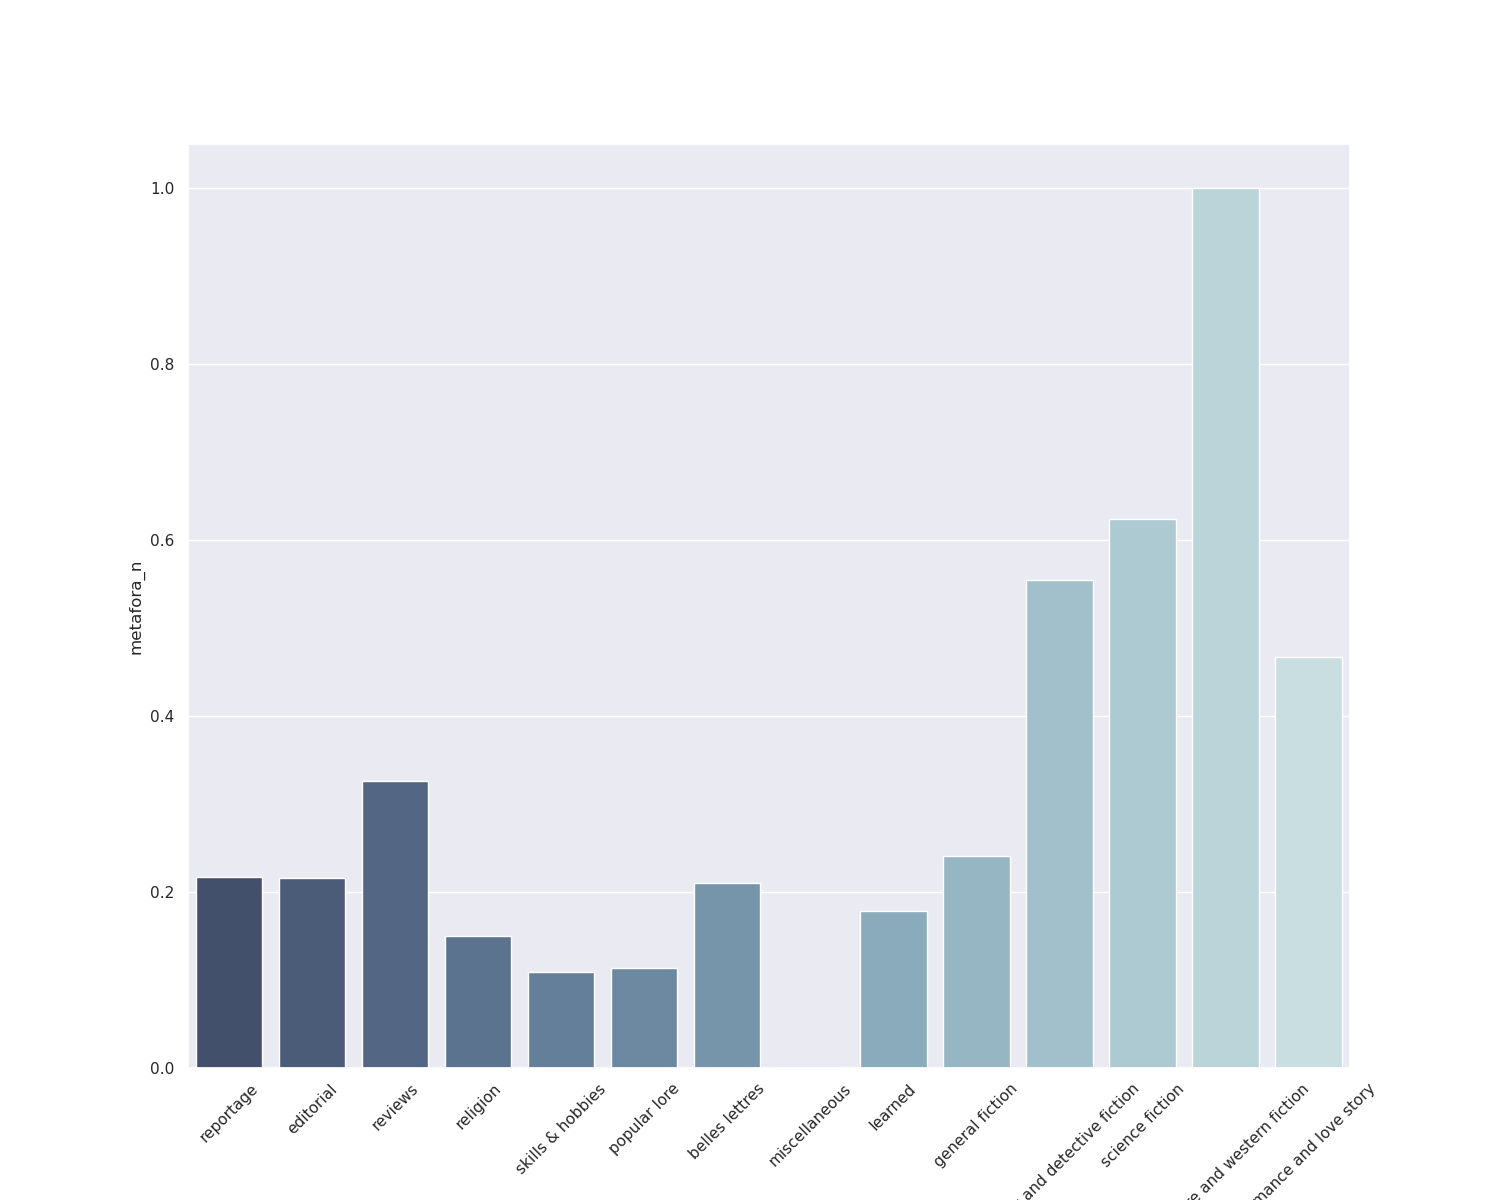
\includegraphics[width=.45\linewidth]{./resultados/graphs/muestra/c1_metafora.png}
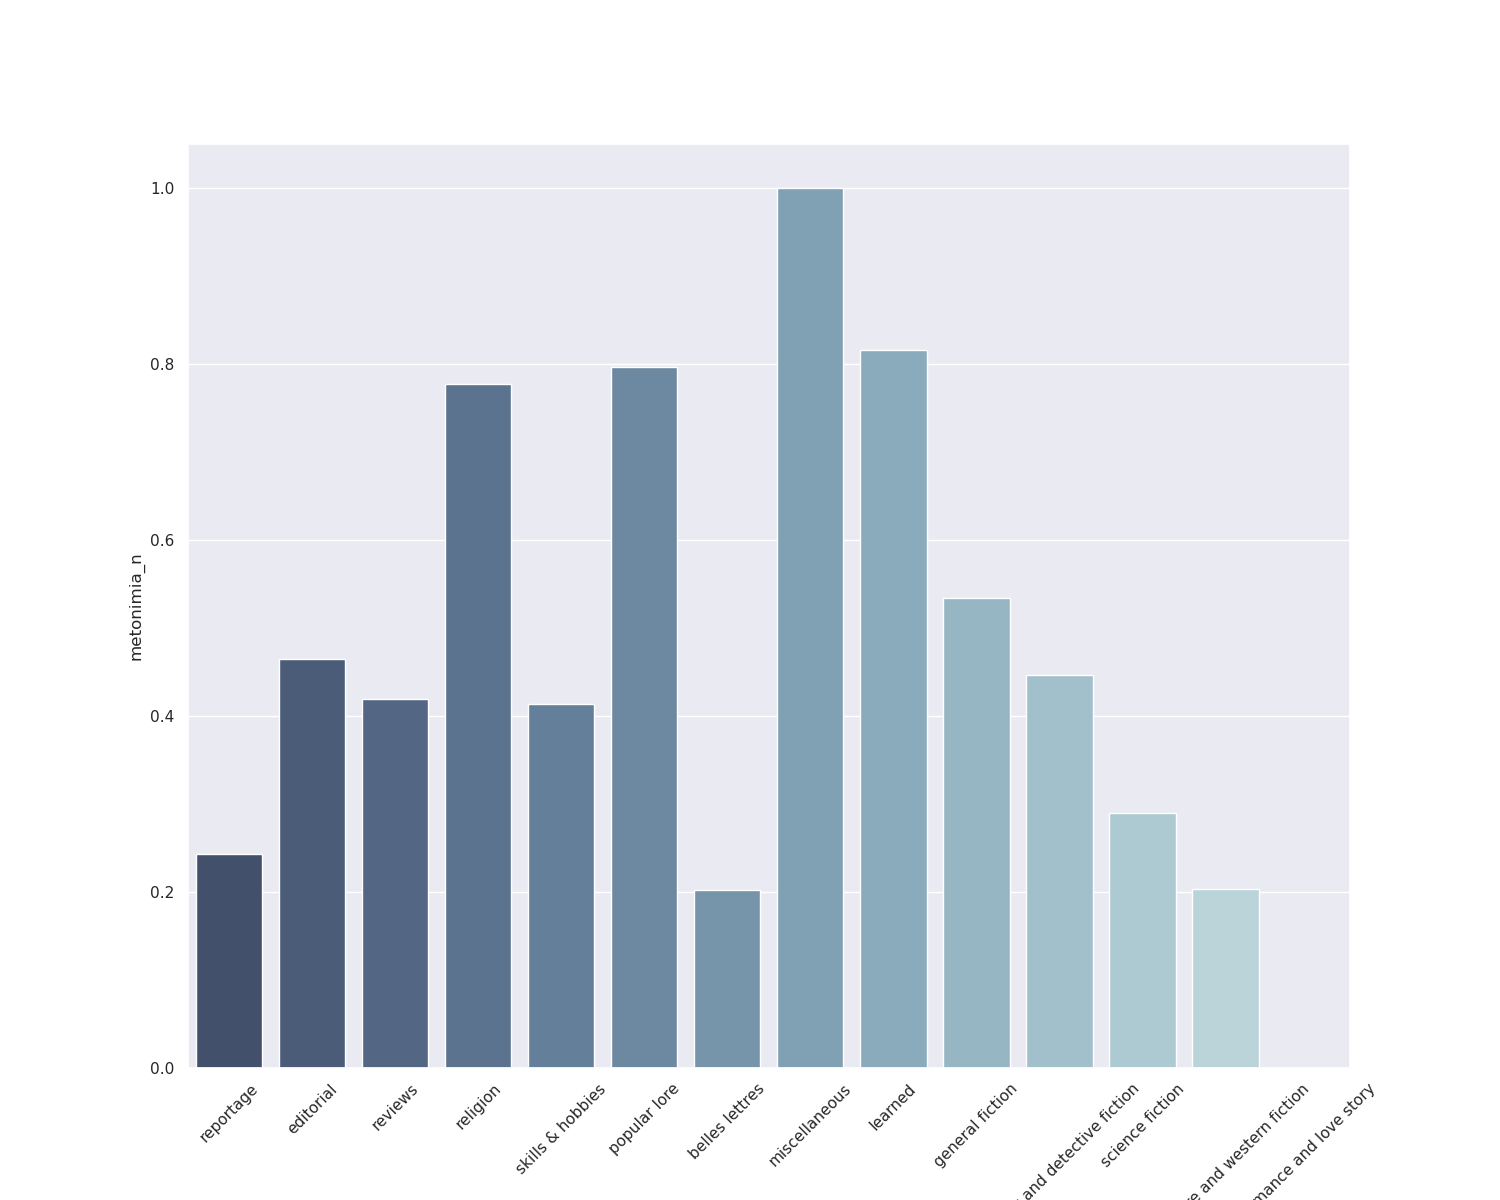
\includegraphics[width=.45\linewidth]{./resultados/graphs/muestra/c1_metonimia.png}
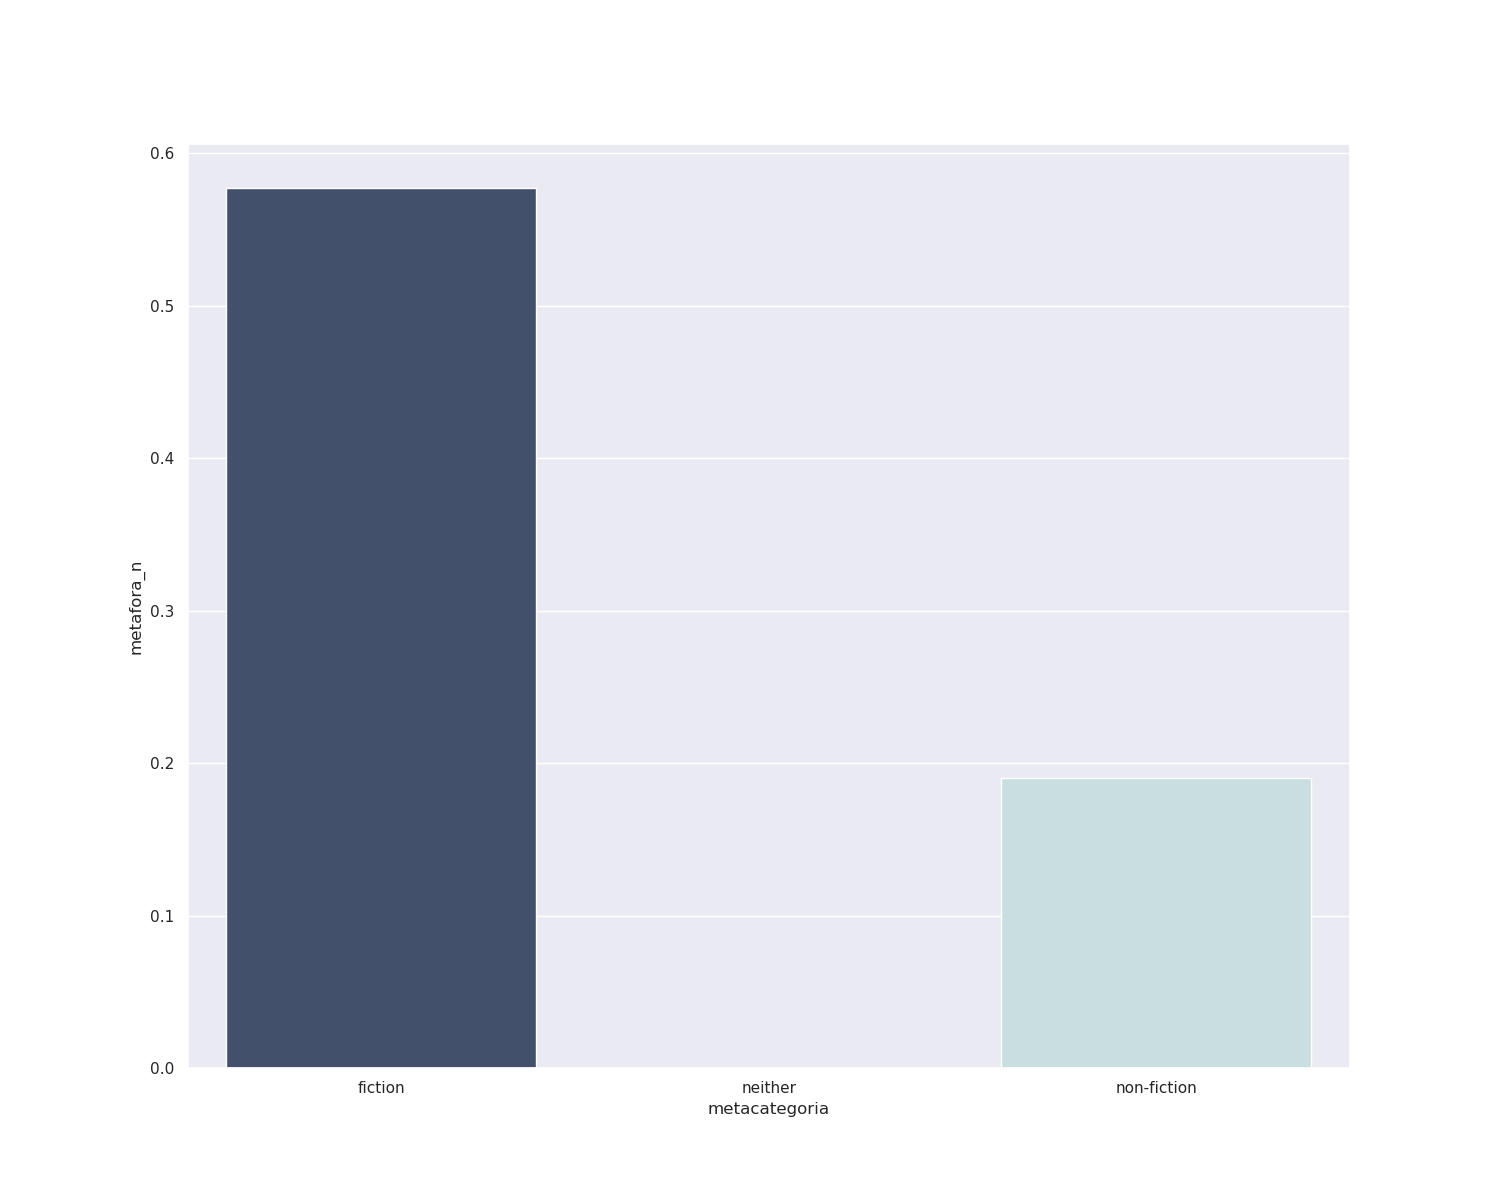
\includegraphics[width=.45\linewidth]{./resultados/graphs/meta/c1_metacategoria_metafora.png}
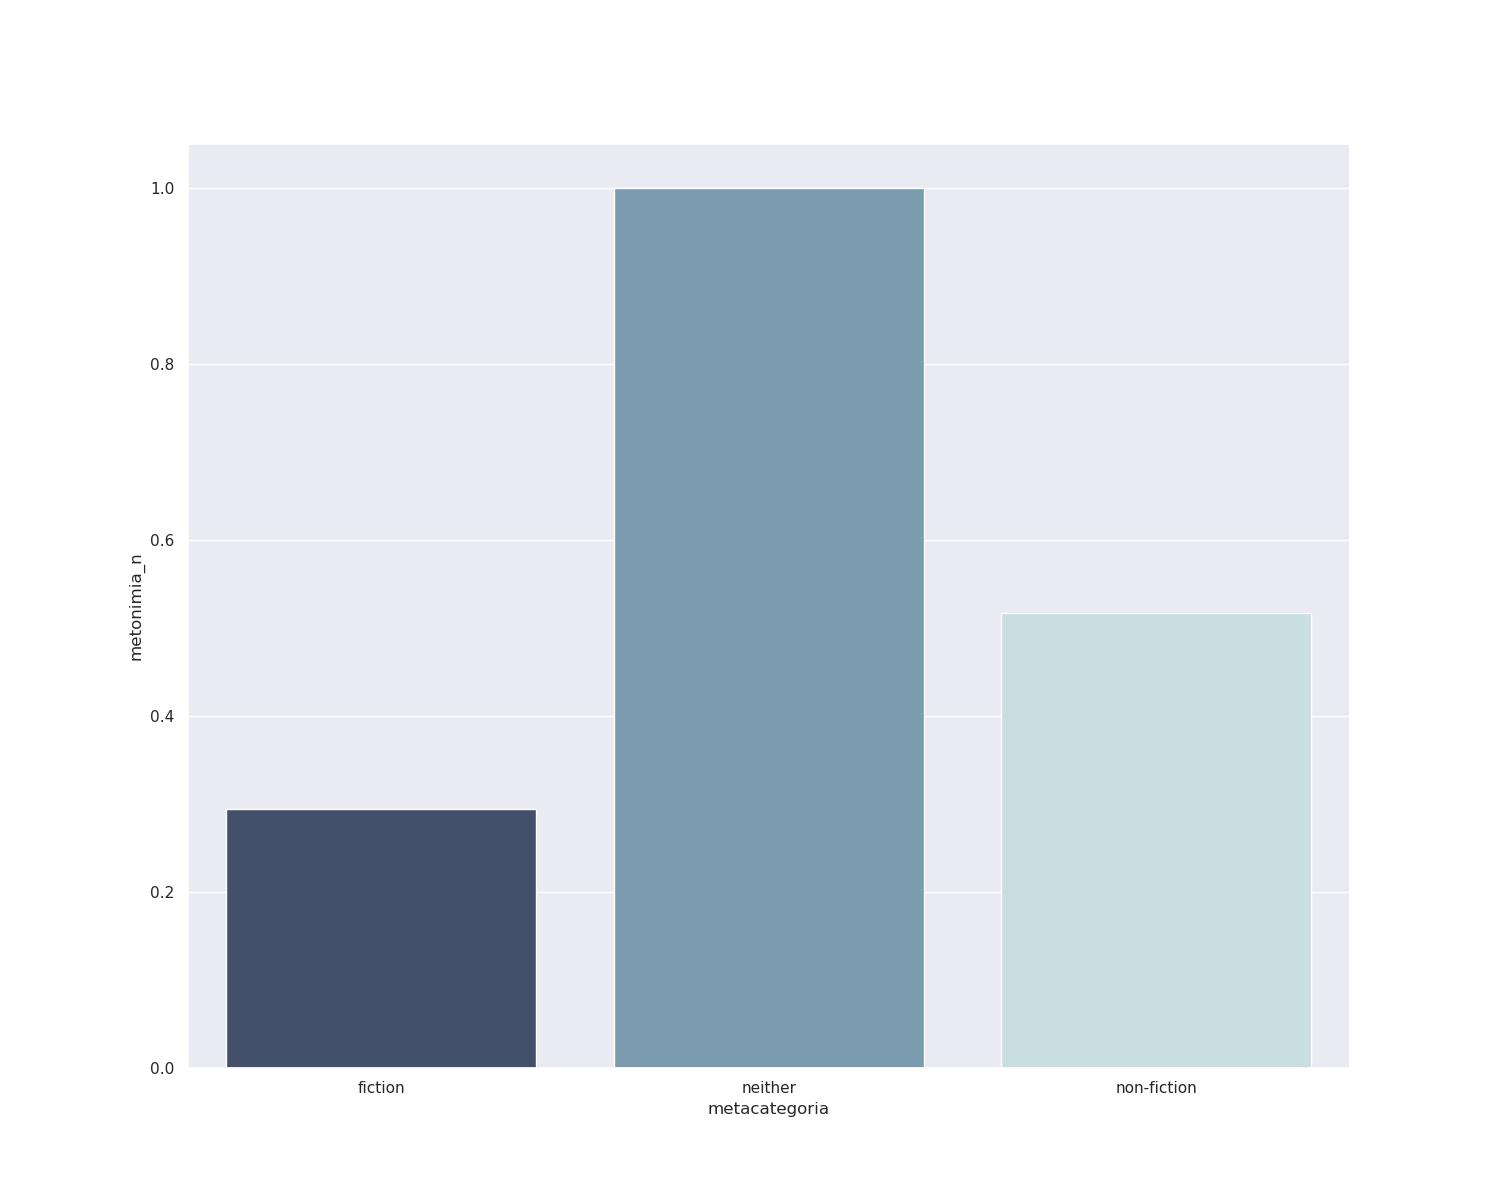
\includegraphics[width=.45\linewidth]{./resultados/graphs/meta/c1_metacategoria_metonimia.png}
\caption{\label{fig:c1_resultados}Resultados muestra 1}
\end{figure}


\begin{figure}[!H]
\centering
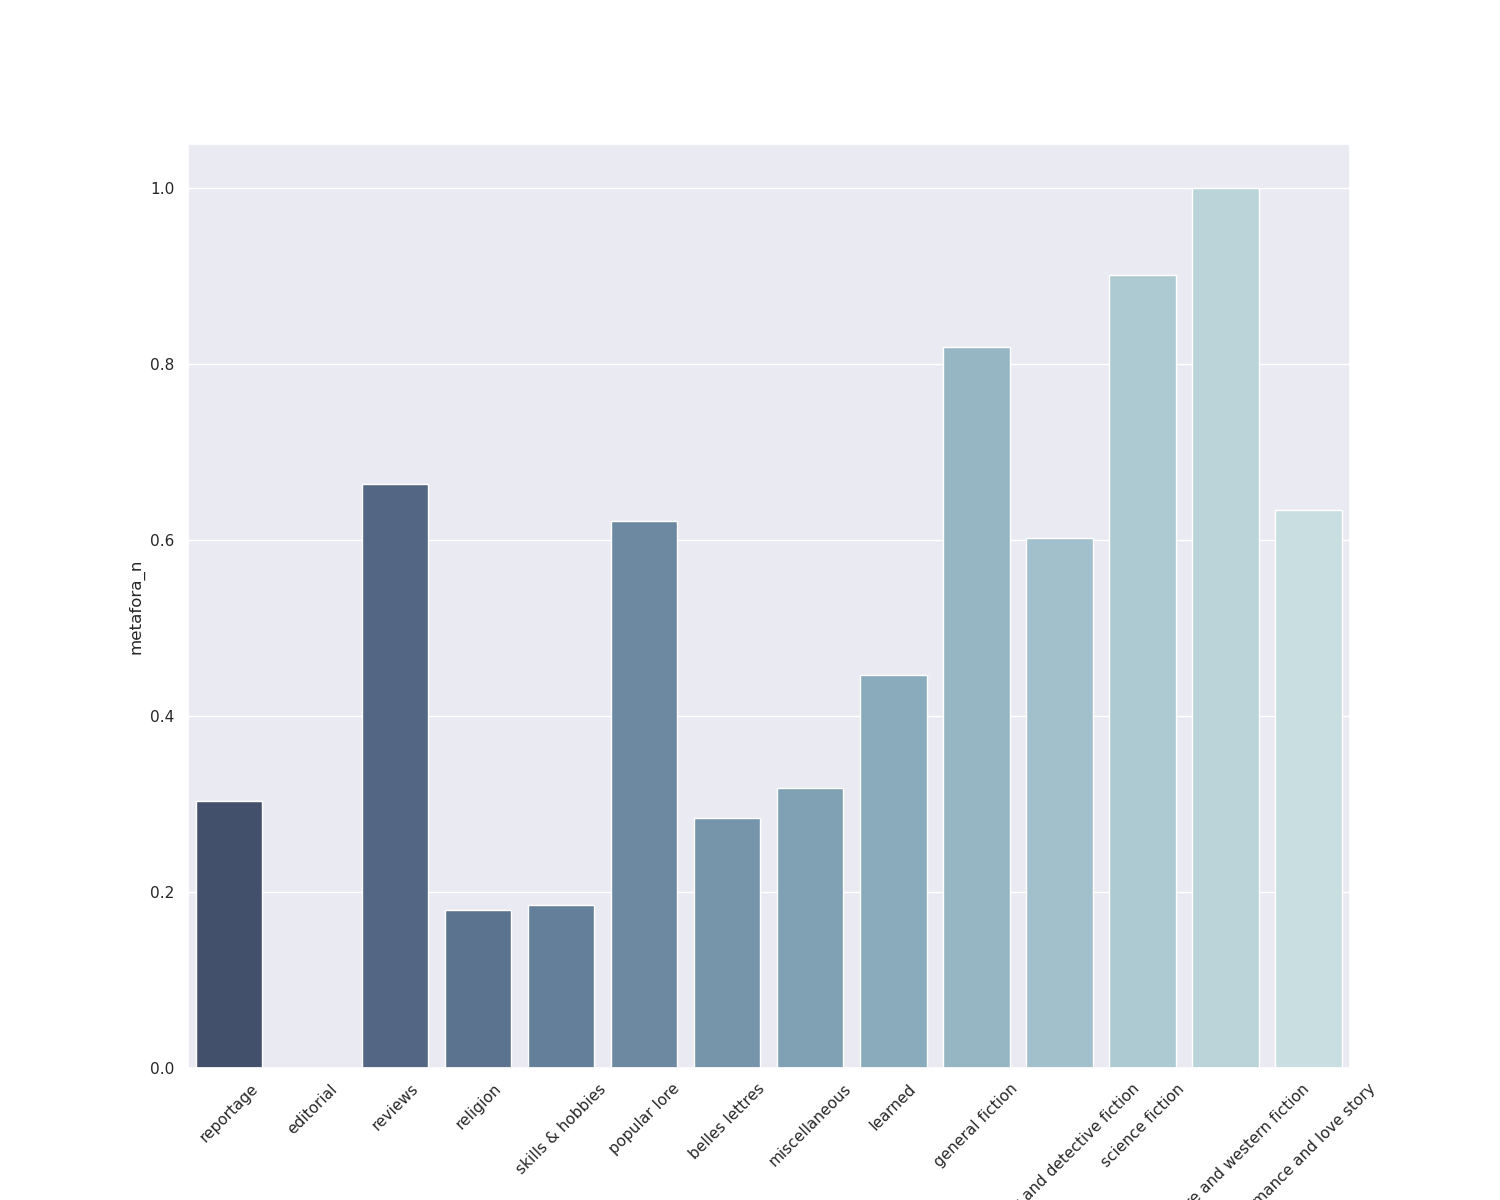
\includegraphics[width=.45\linewidth]{./resultados/graphs/muestra/c2_metafora.png}
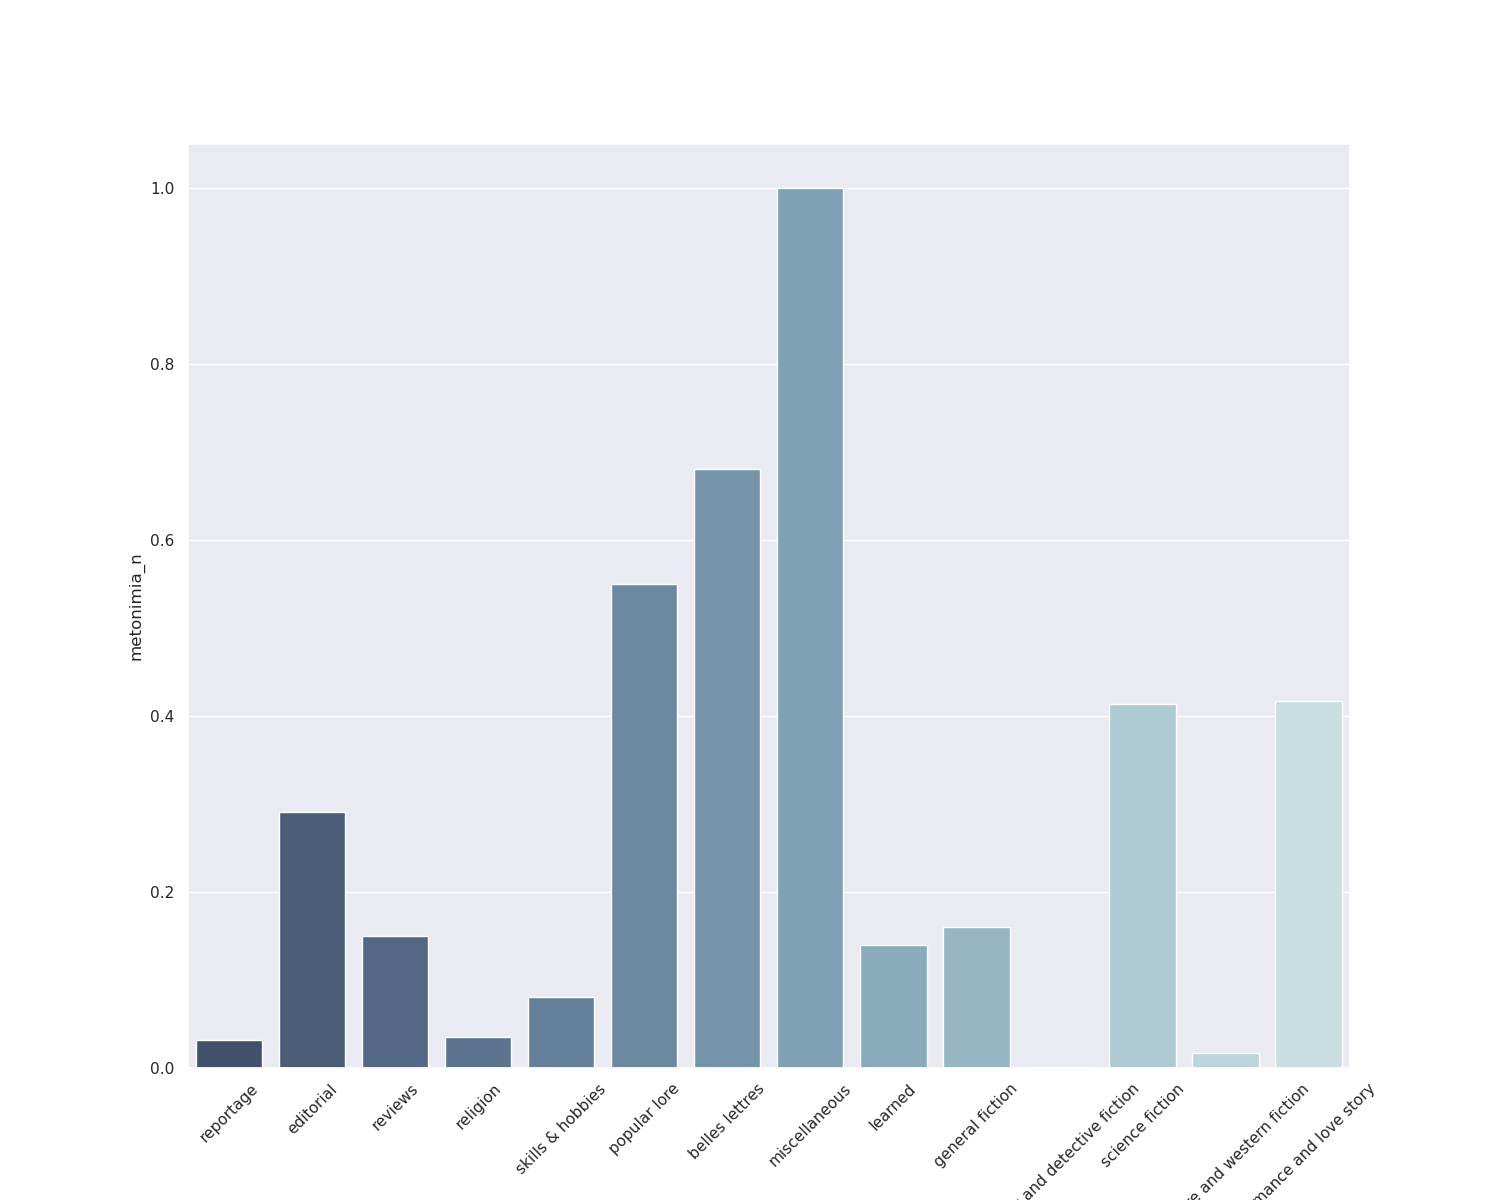
\includegraphics[width=.45\linewidth]{./resultados/graphs/muestra/c2_metonimia.png}
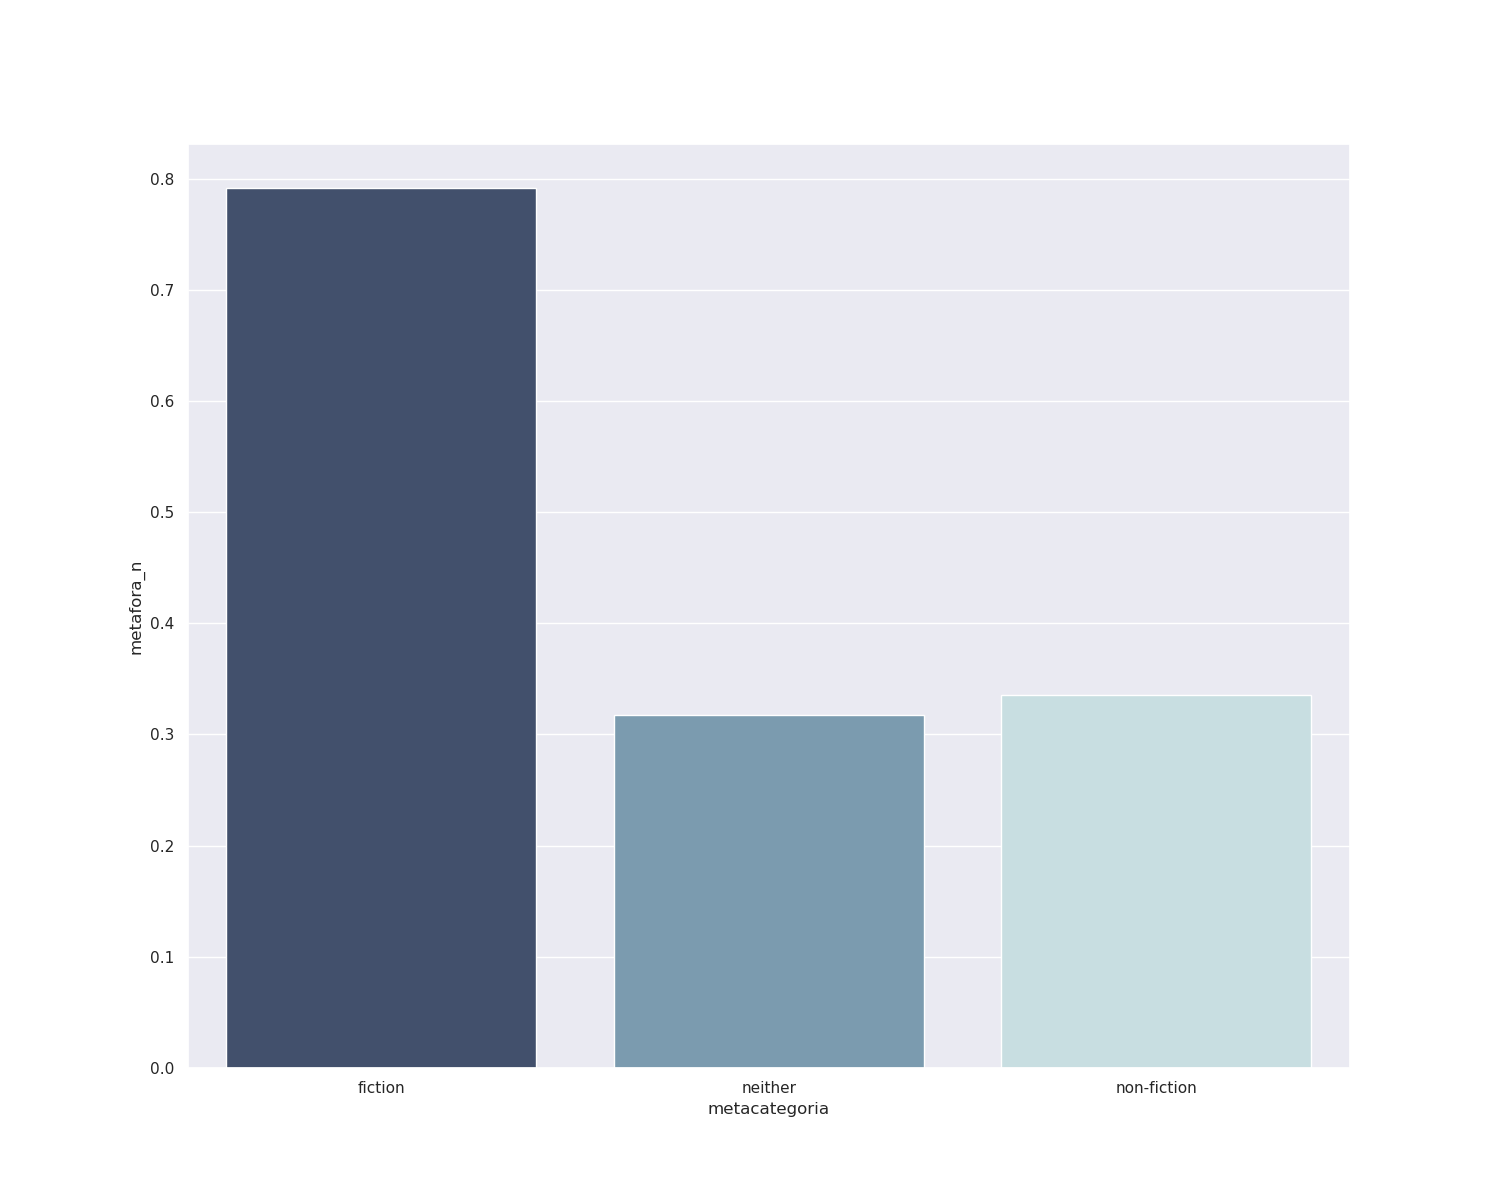
\includegraphics[width=.45\linewidth]{./resultados/graphs/meta/c2_metacategoria_metafora.png}
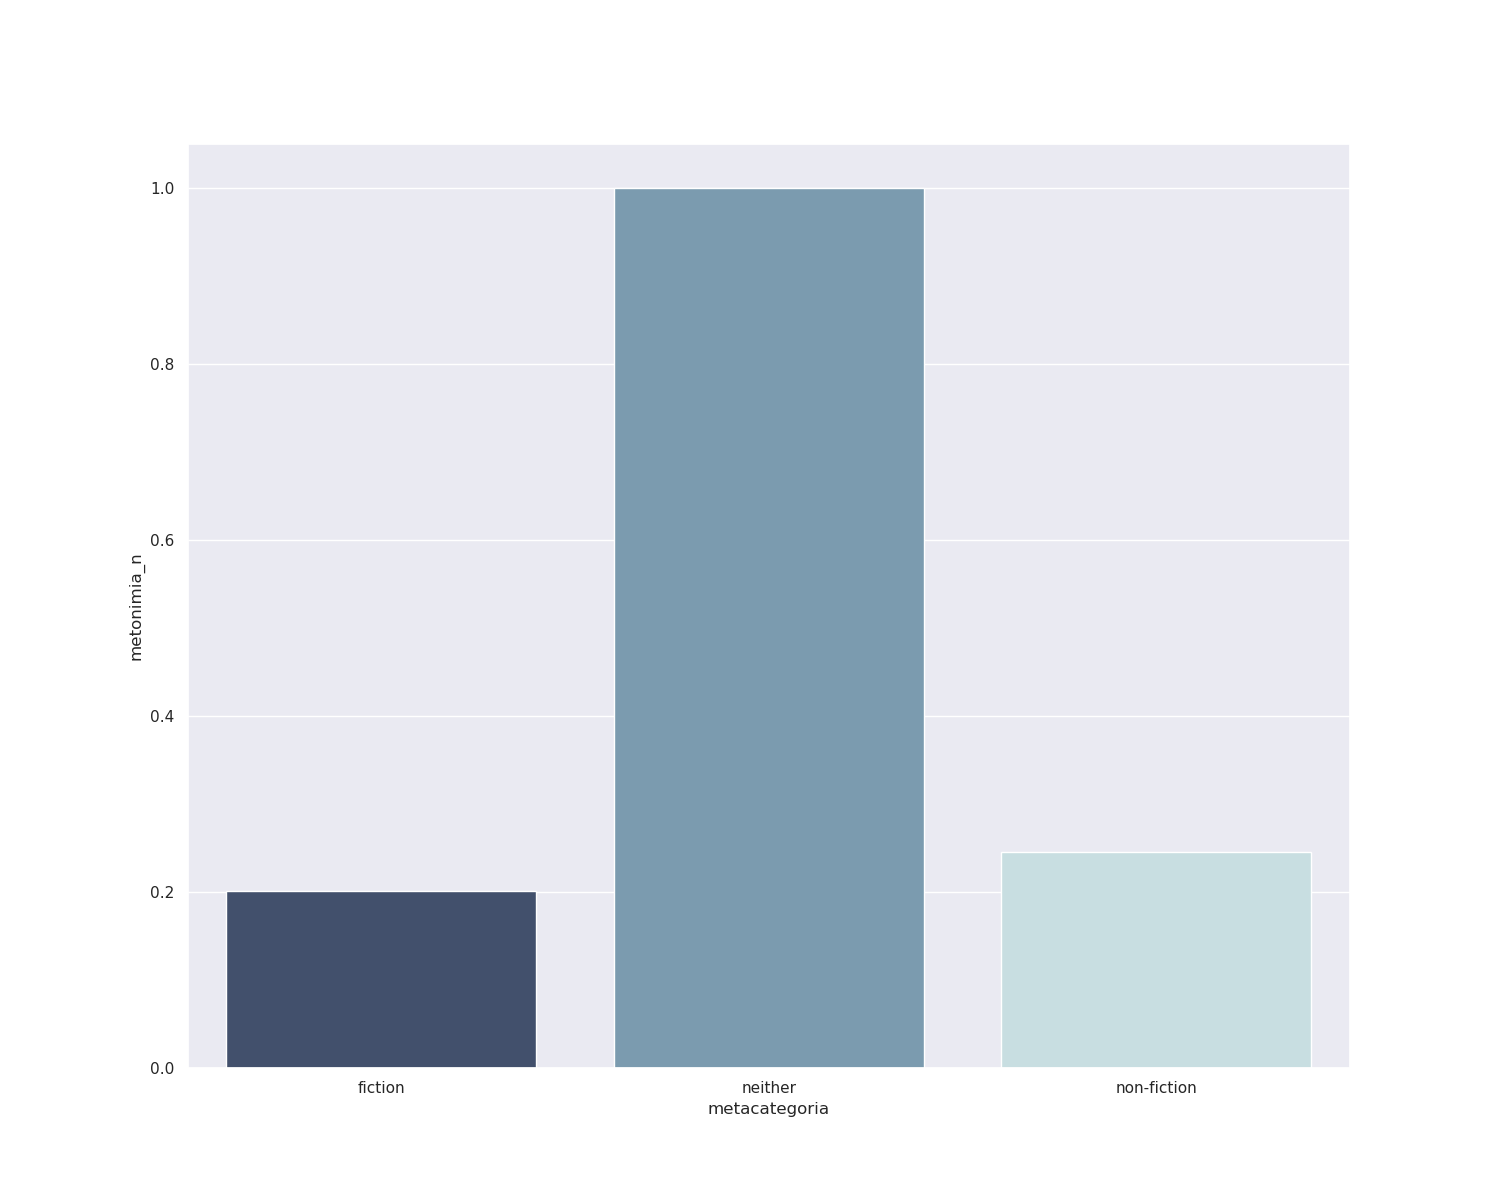
\includegraphics[width=.45\linewidth]{./resultados/graphs/meta/c2_metacategoria_metonimia.png}
\caption{\label{fig:c2_resultados}Resultados muestra 2}
\end{figure}

\begin{figure}[!H]
\centering
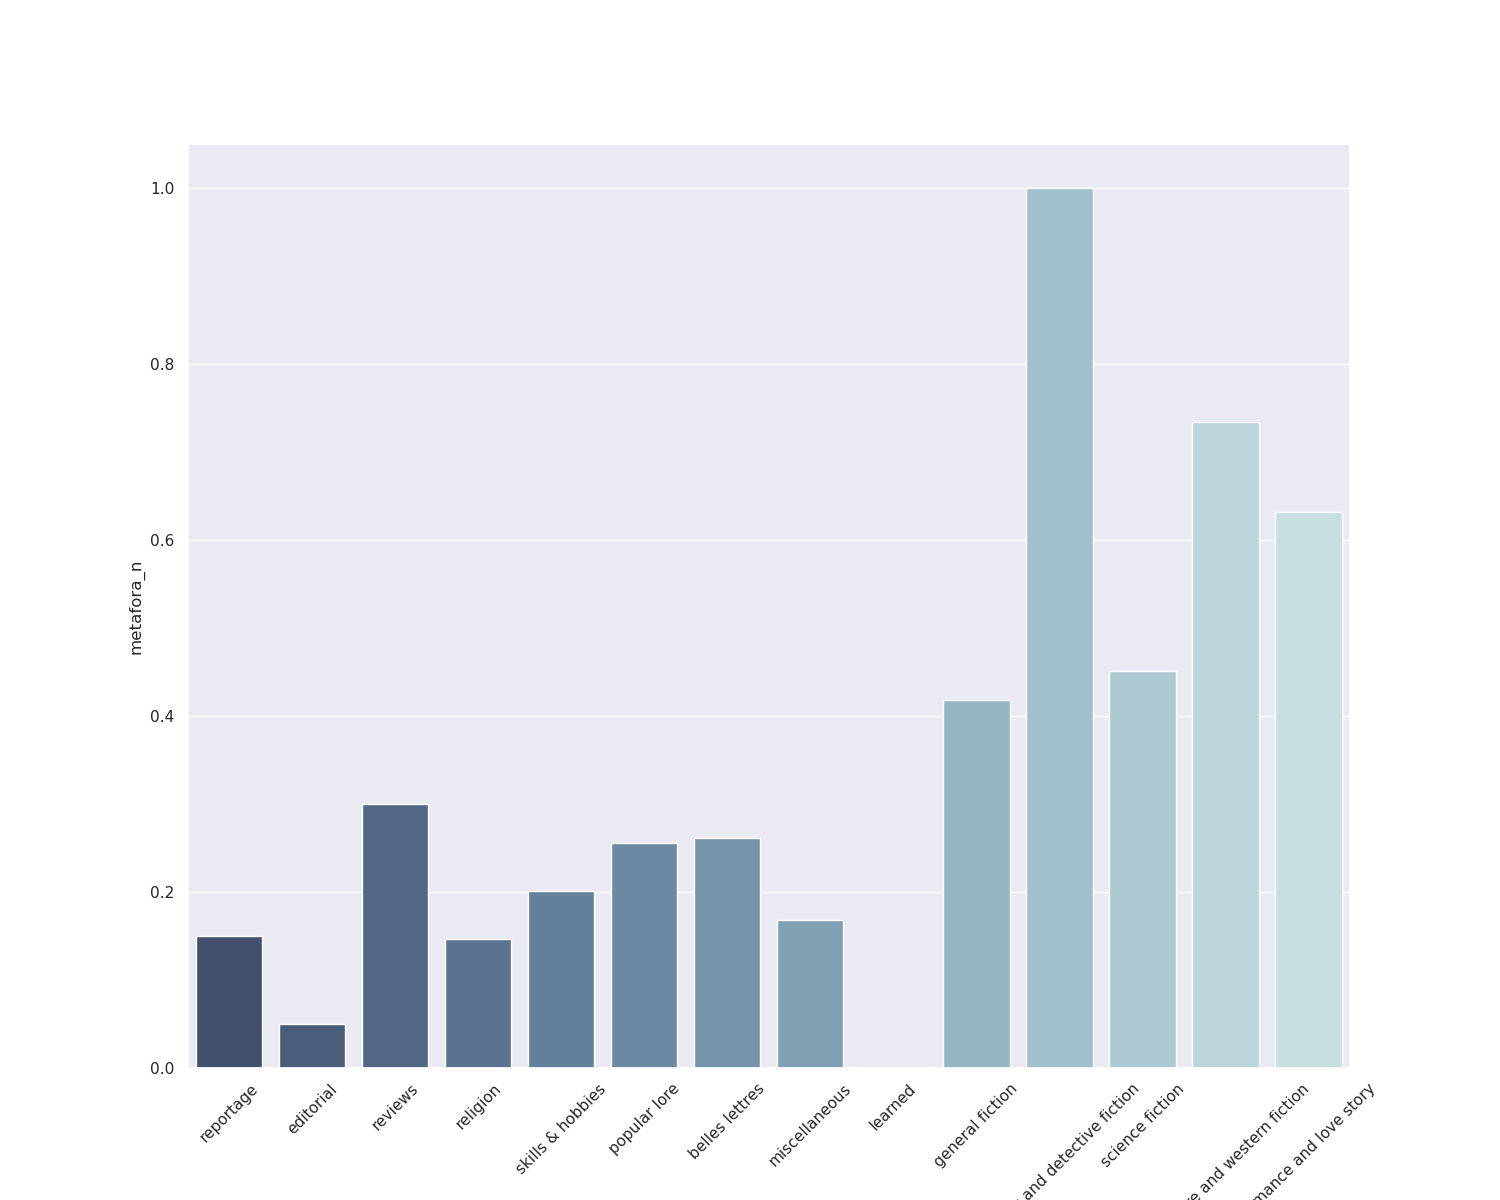
\includegraphics[width=.45\linewidth]{./resultados/graphs/muestra/c3_metafora.png}
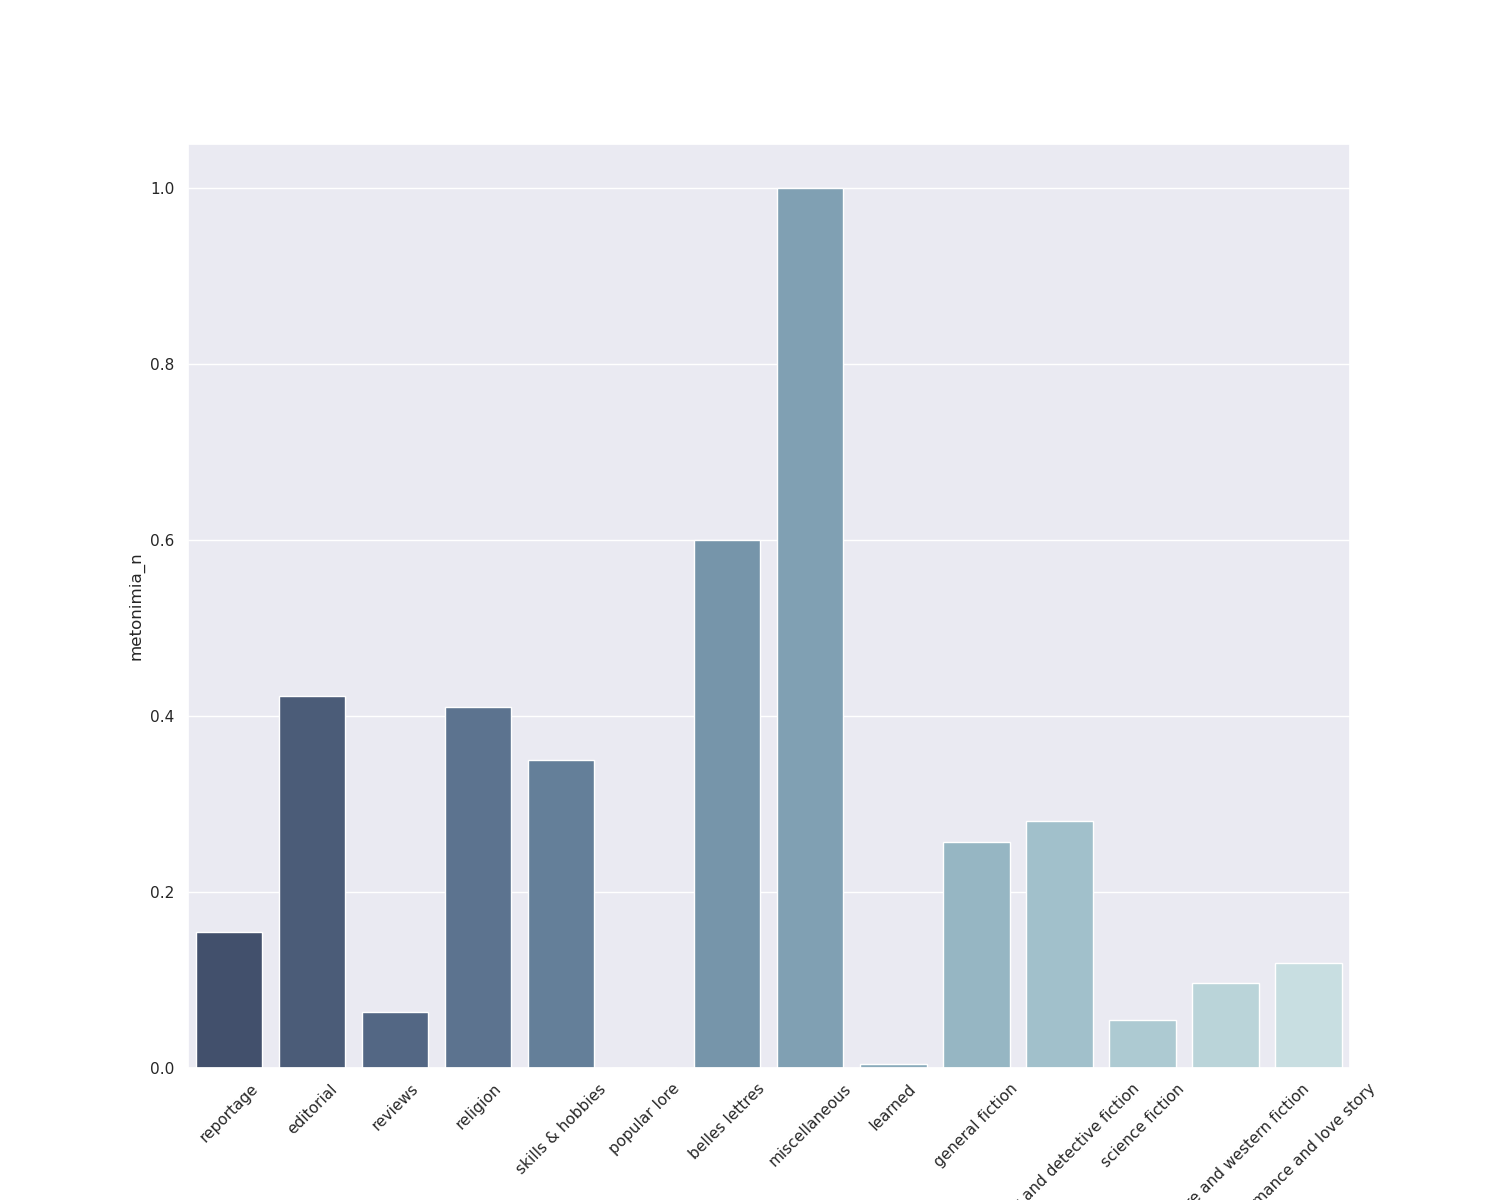
\includegraphics[width=.45\linewidth]{./resultados/graphs/muestra/c3_metonimia.png}
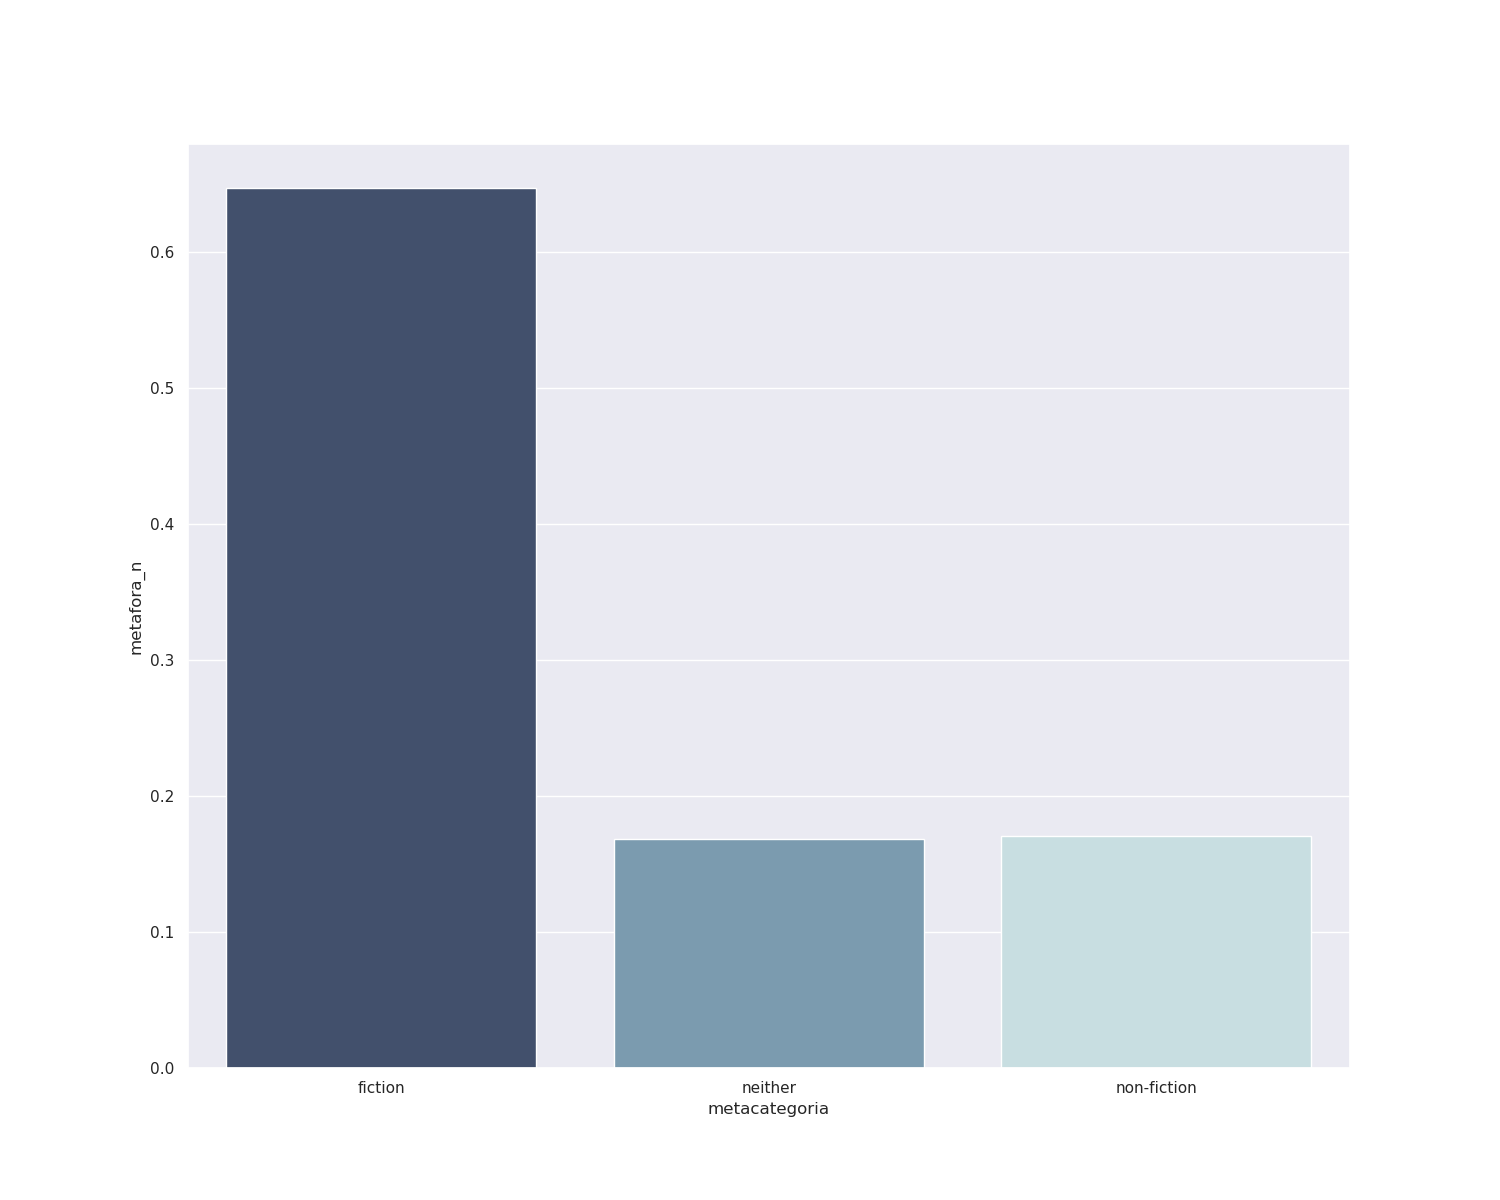
\includegraphics[width=.45\linewidth]{./resultados/graphs/meta/c3_metacategoria_metafora.png}
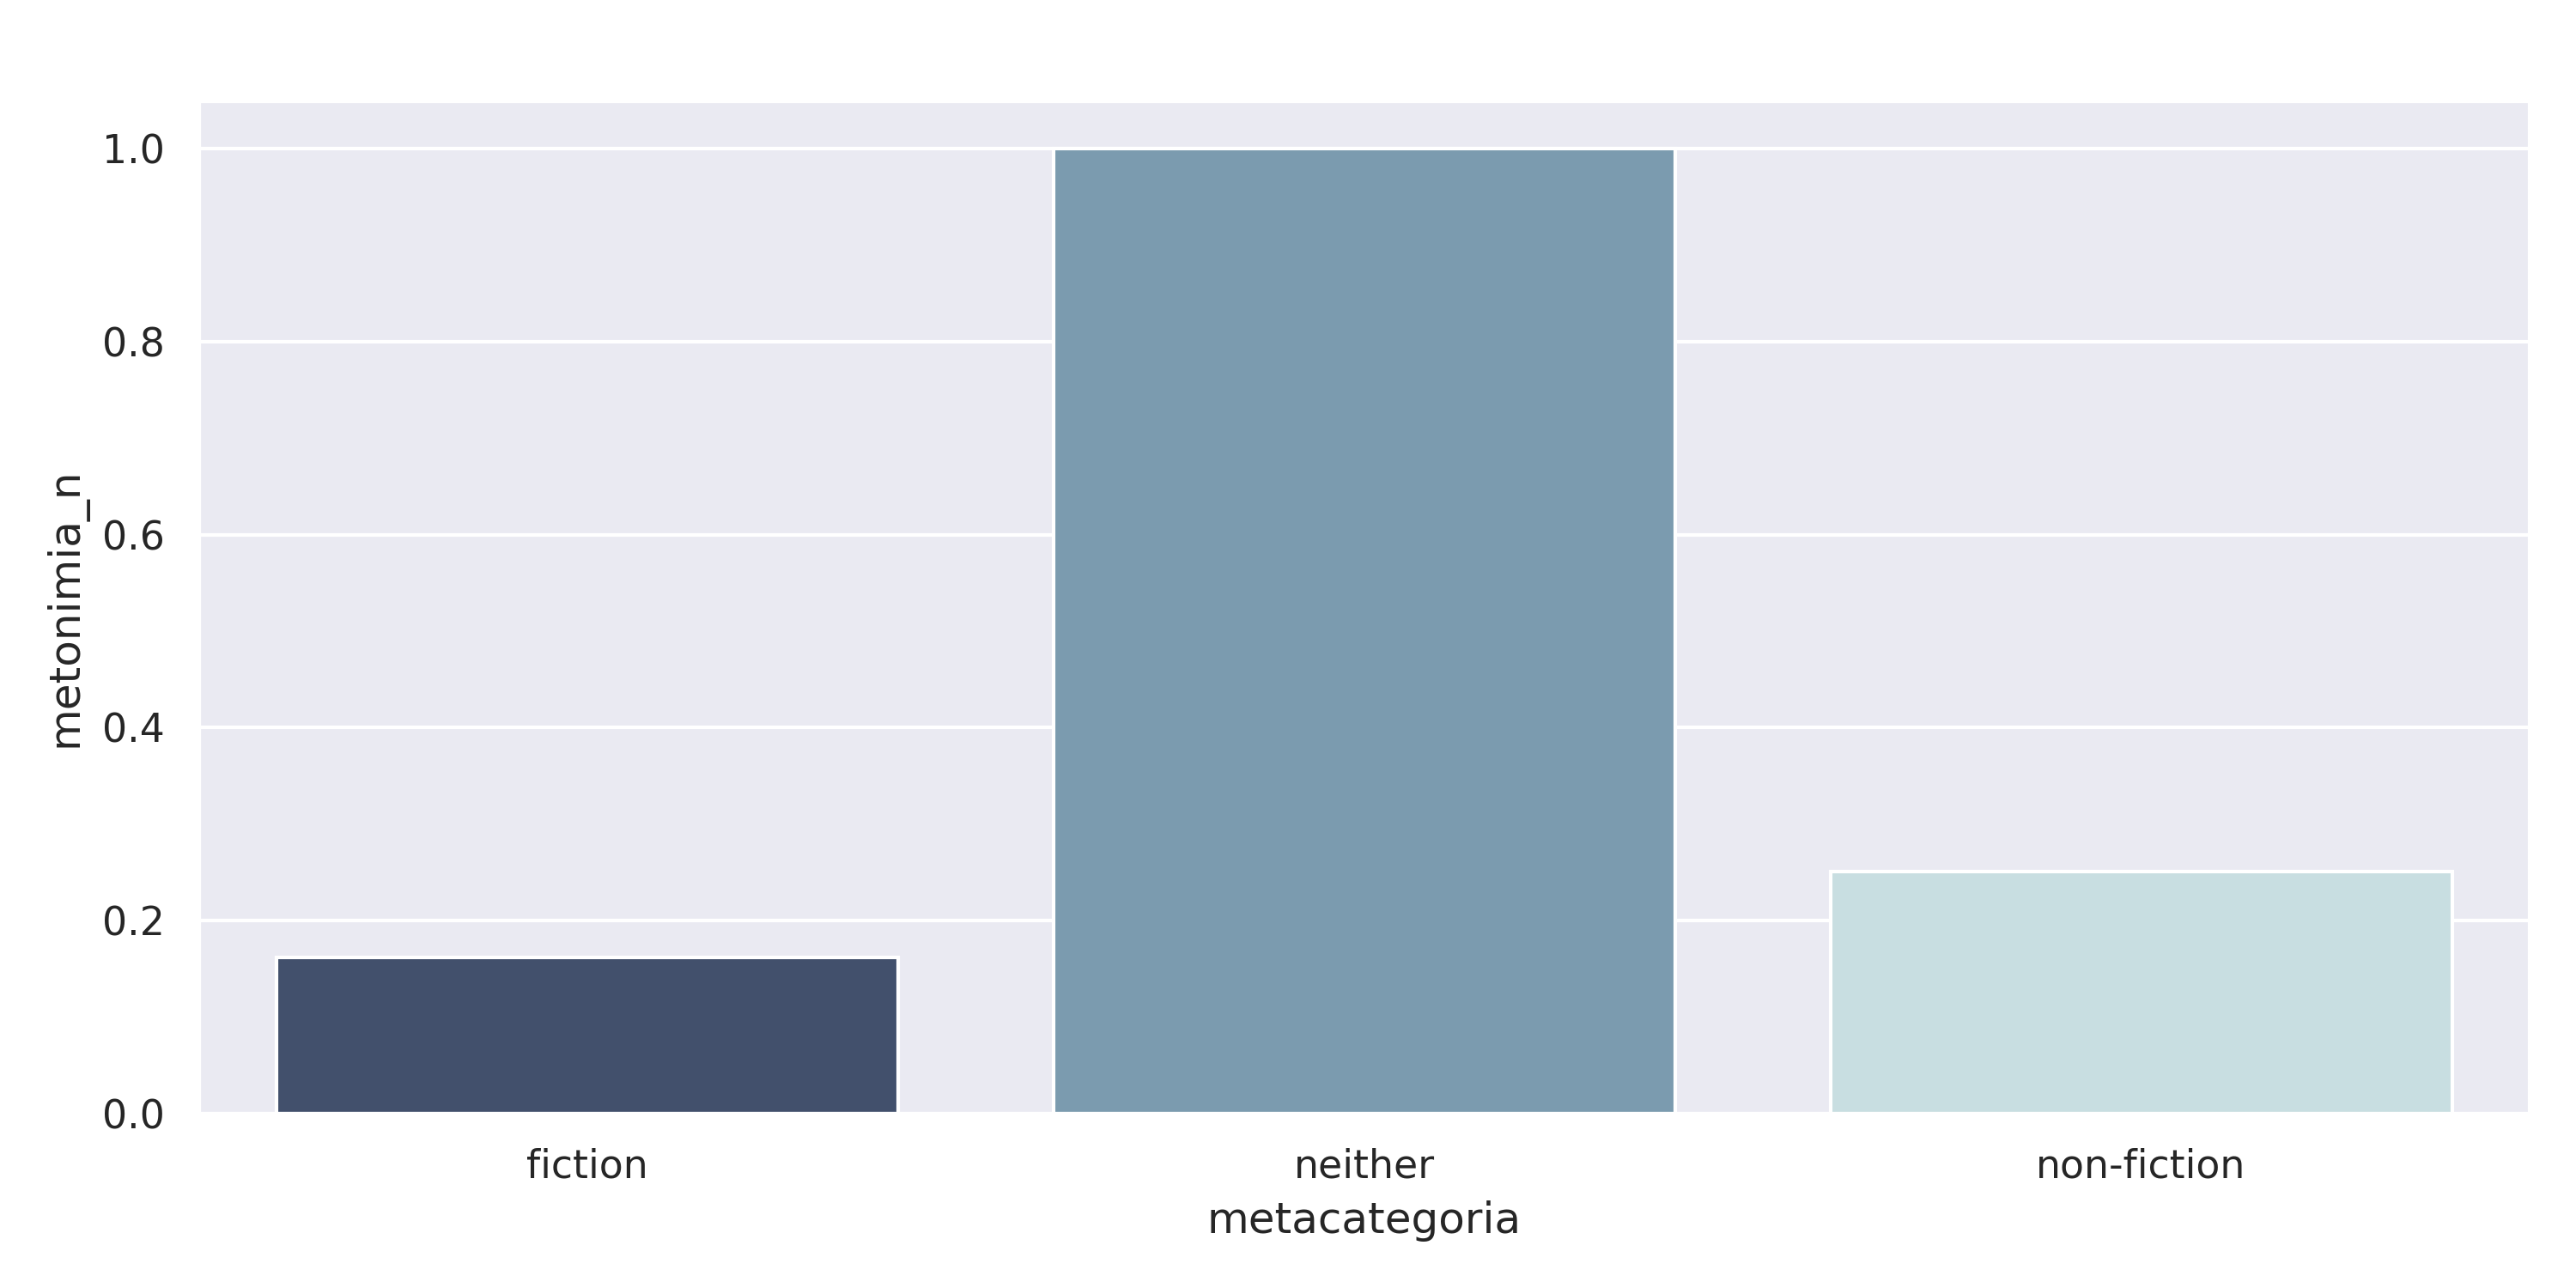
\includegraphics[width=.45\linewidth]{./resultados/graphs/meta/c3_metacategoria_metonimia.png}
\caption{\label{fig:c3_resultados}Resultados muestra 3}
\end{figure}

\begin{figure}[!H]
\centering
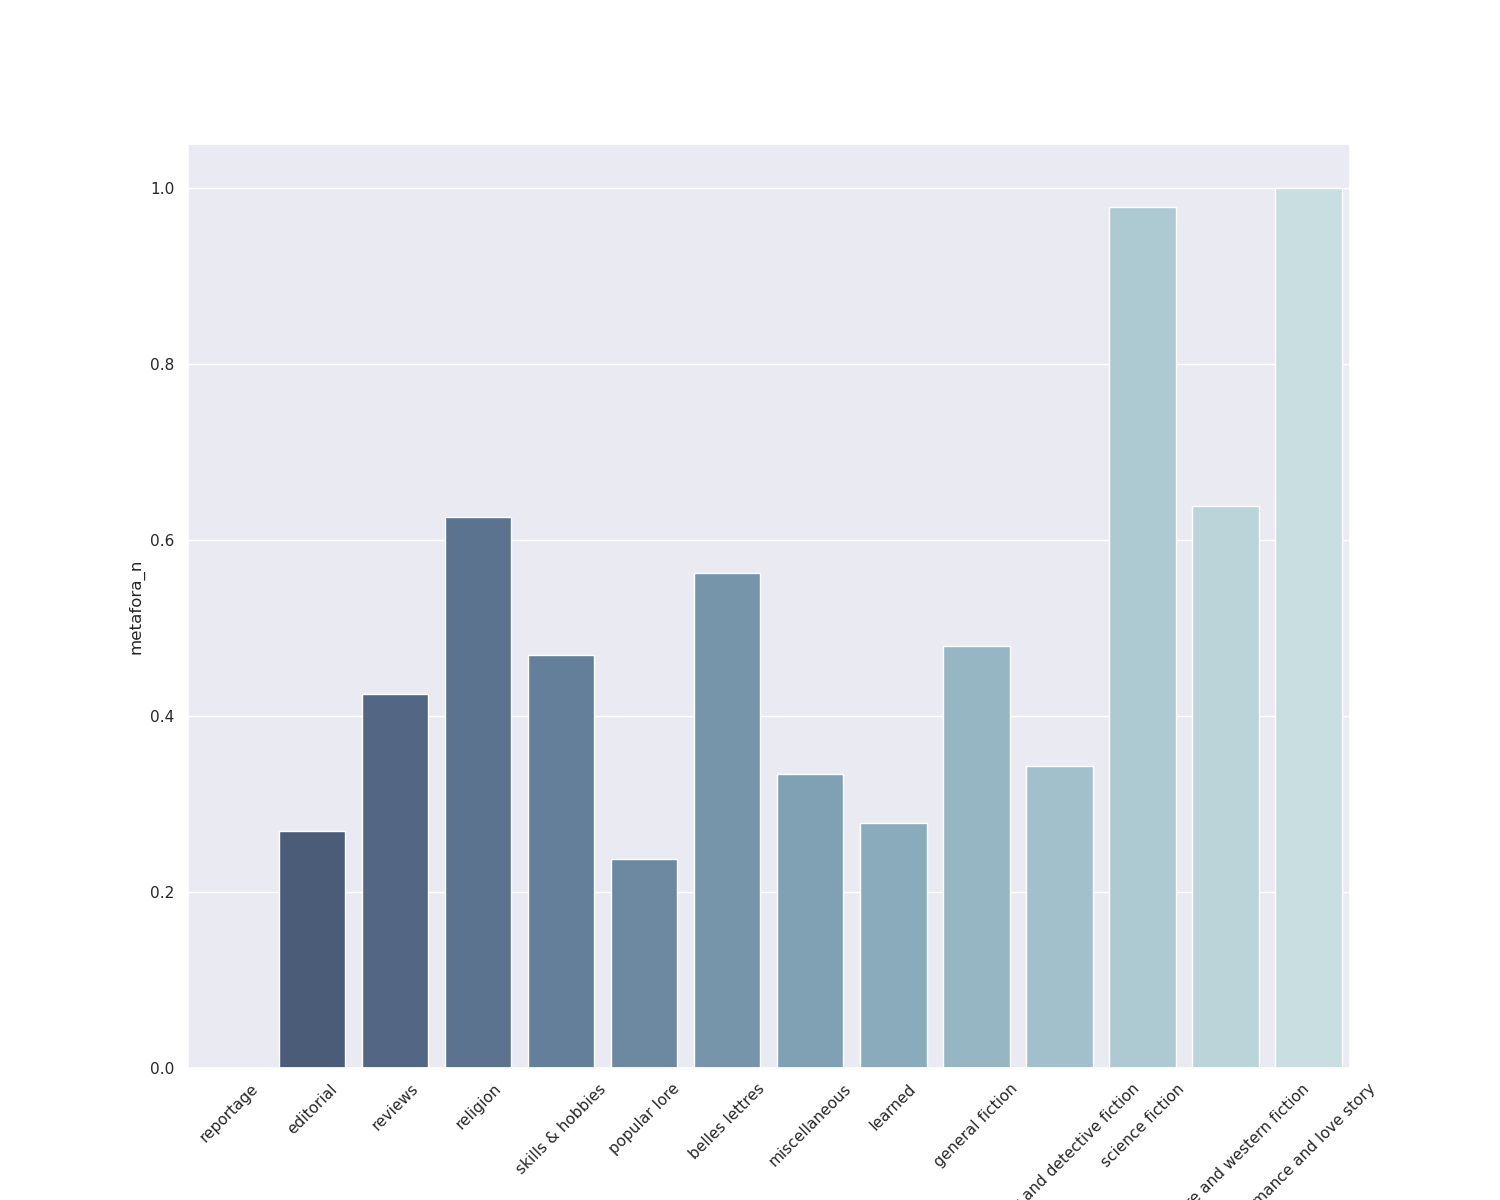
\includegraphics[width=.45\linewidth]{./resultados/graphs/muestra/c4_metafora.png}
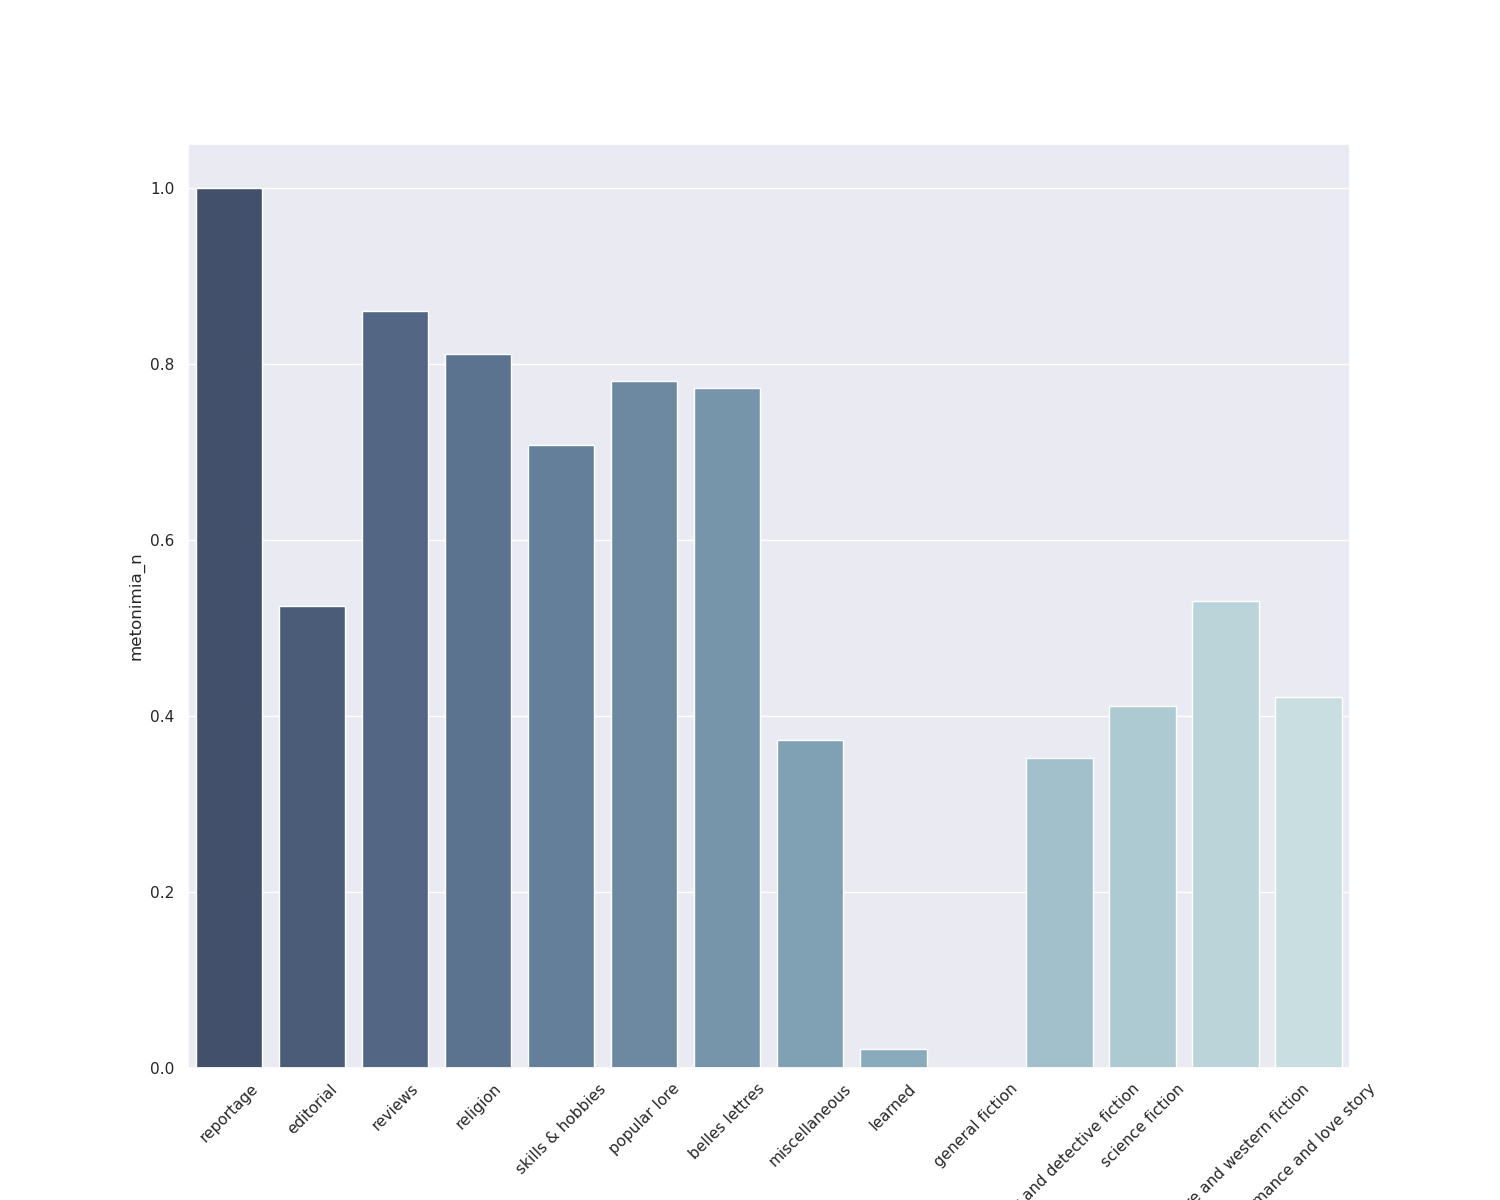
\includegraphics[width=.45\linewidth]{./resultados/graphs/muestra/c4_metonimia.png}
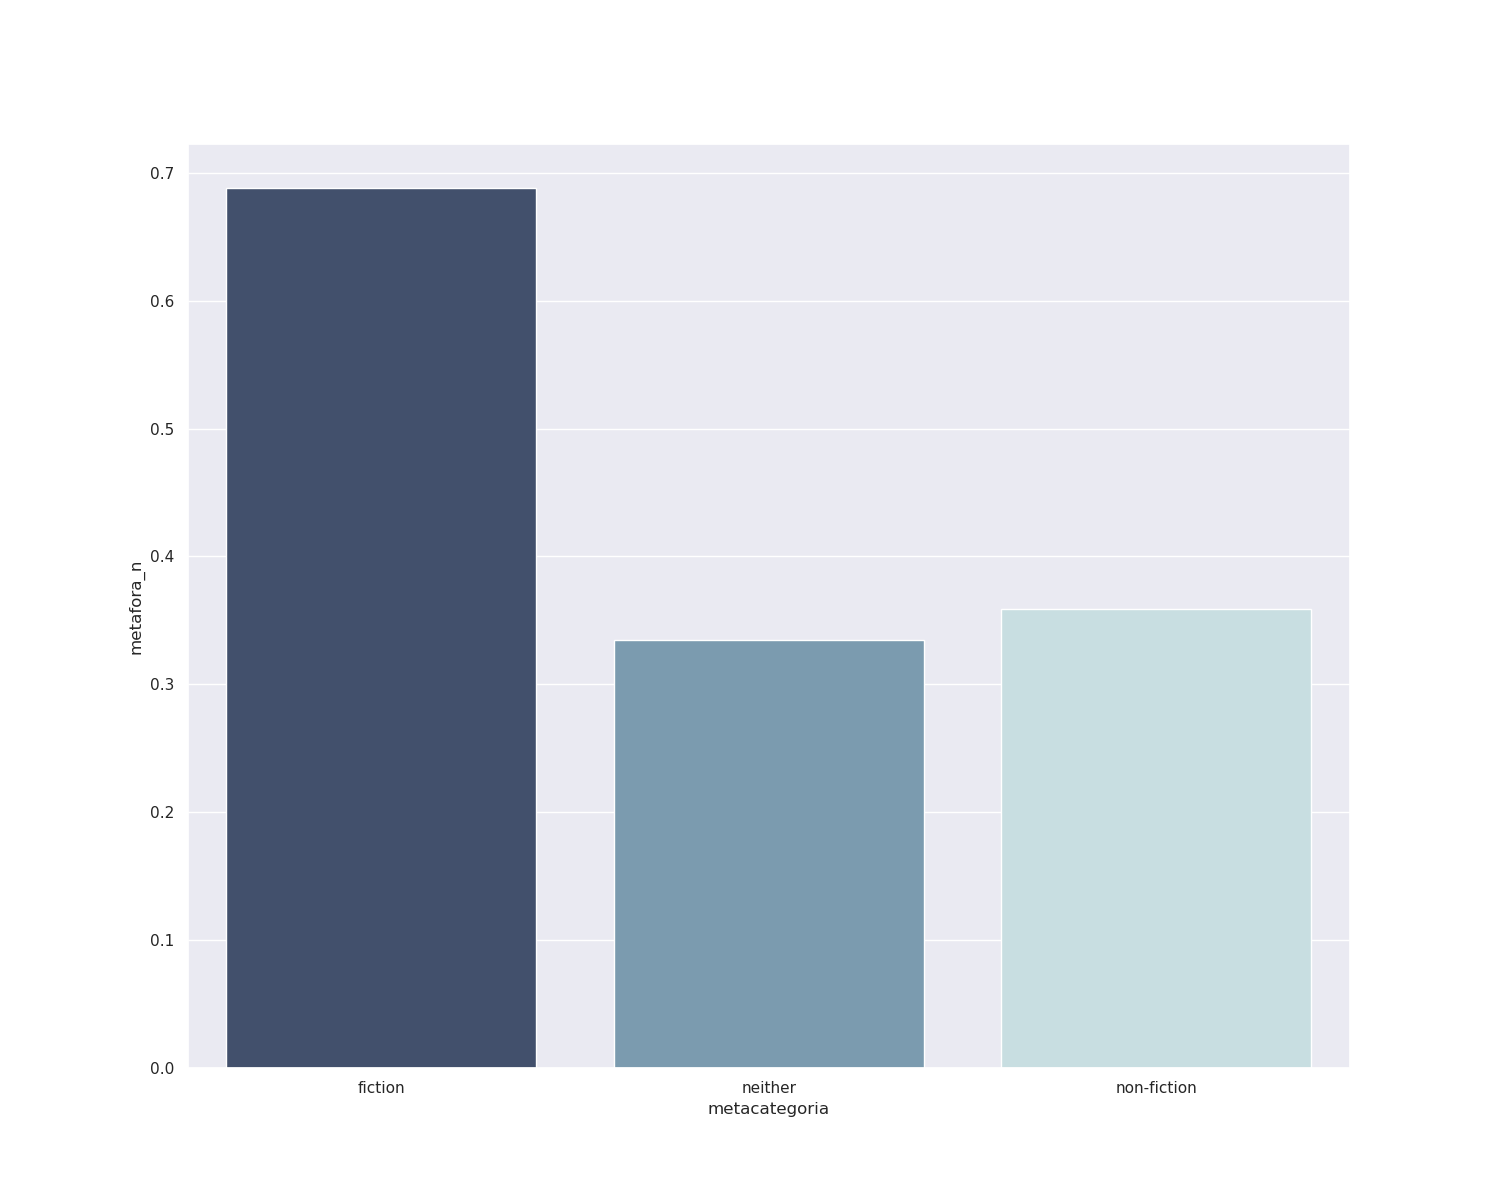
\includegraphics[width=.45\linewidth]{./resultados/graphs/meta/c4_metacategoria_metafora.png}
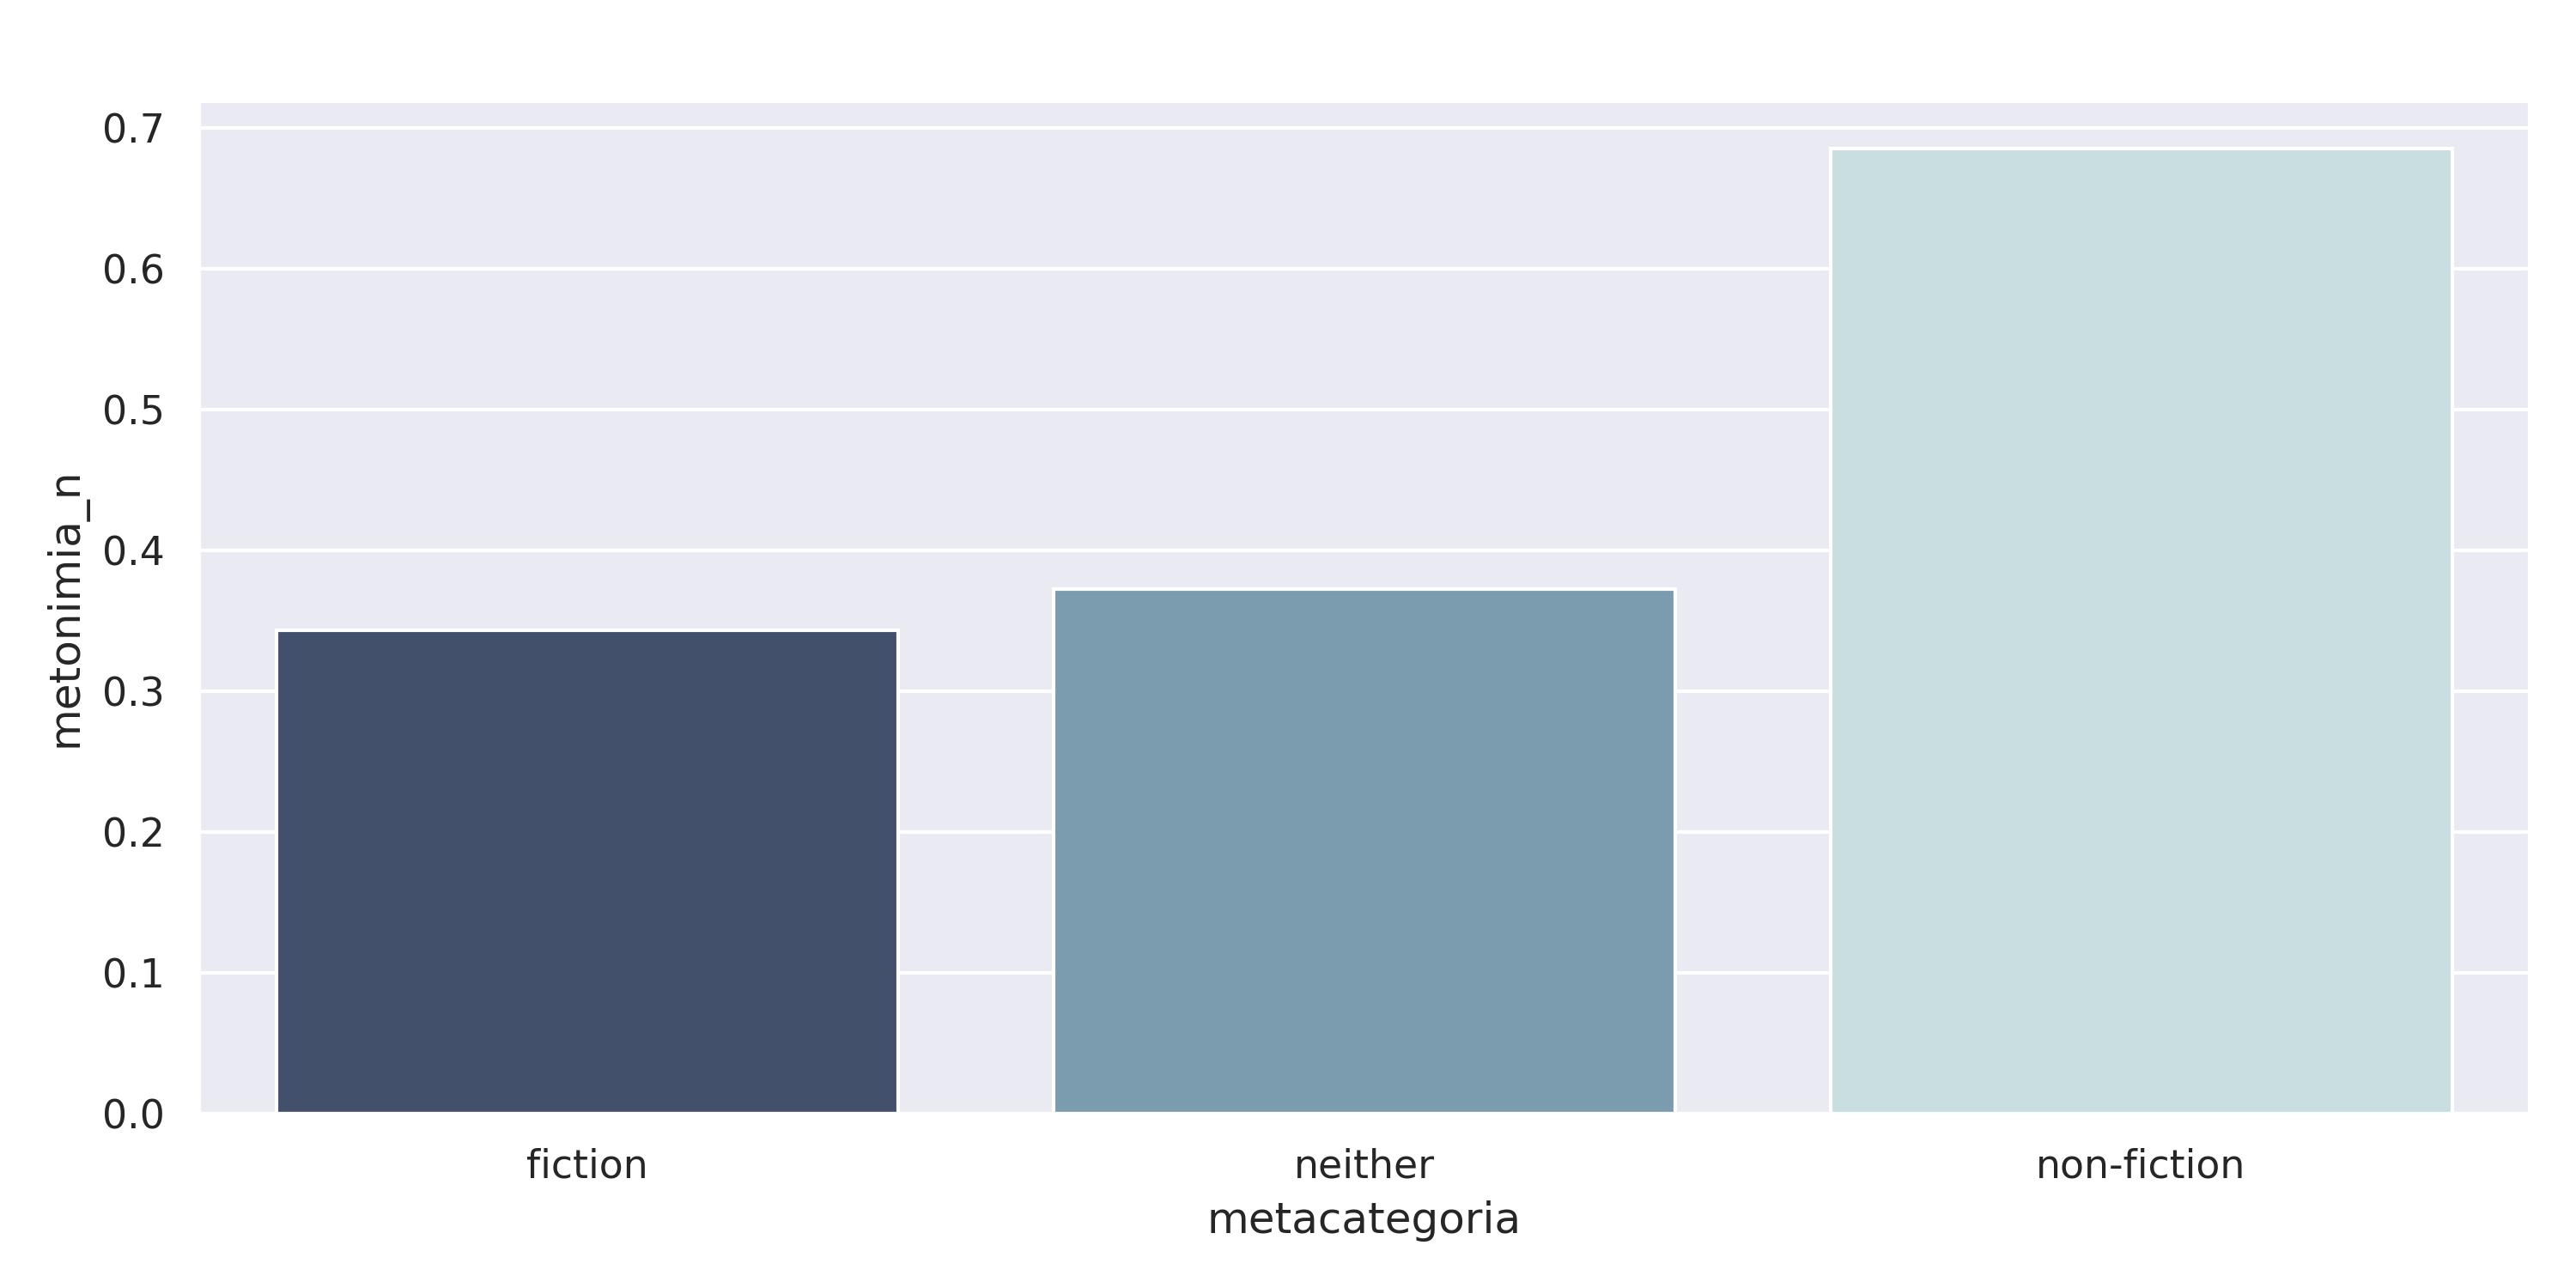
\includegraphics[width=.45\linewidth]{./resultados/graphs/meta/c4_metacategoria_metonimia.png}
\caption{\label{fig:c4_resultados}Resultados muestra 4}
\end{figure}

\begin{figure}[!H]
\centering
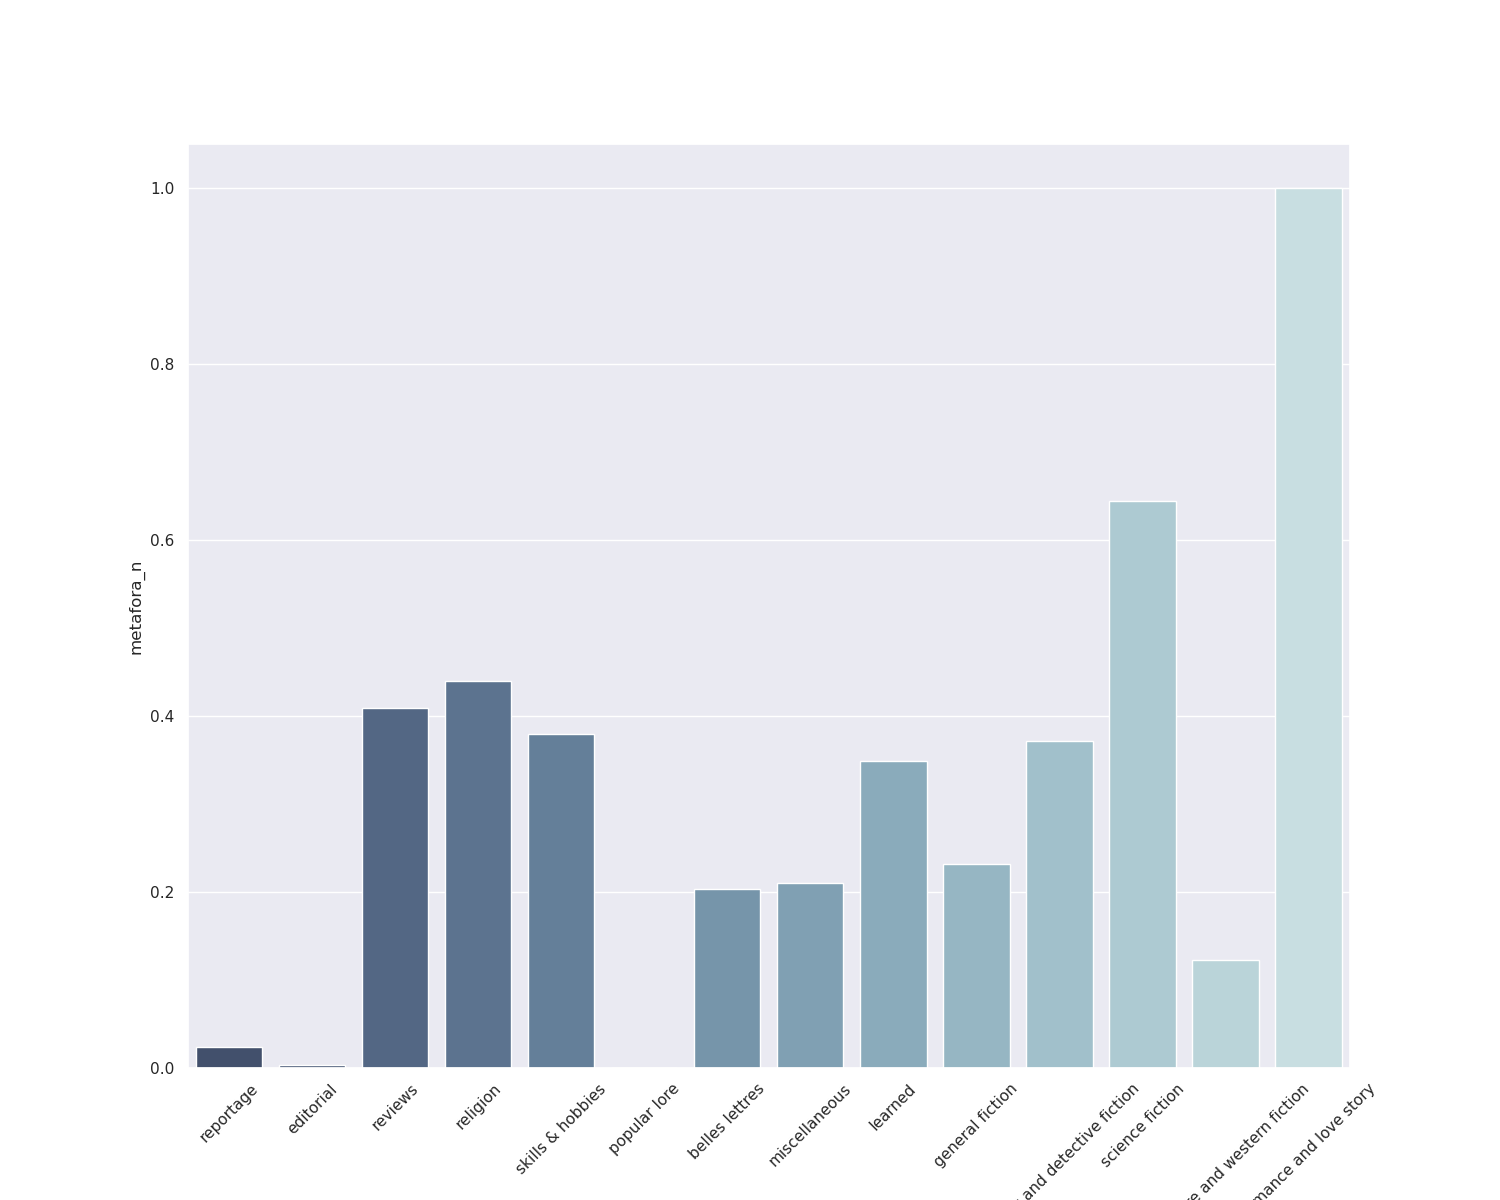
\includegraphics[width=.45\linewidth]{./resultados/graphs/muestra/c5_metafora.png}
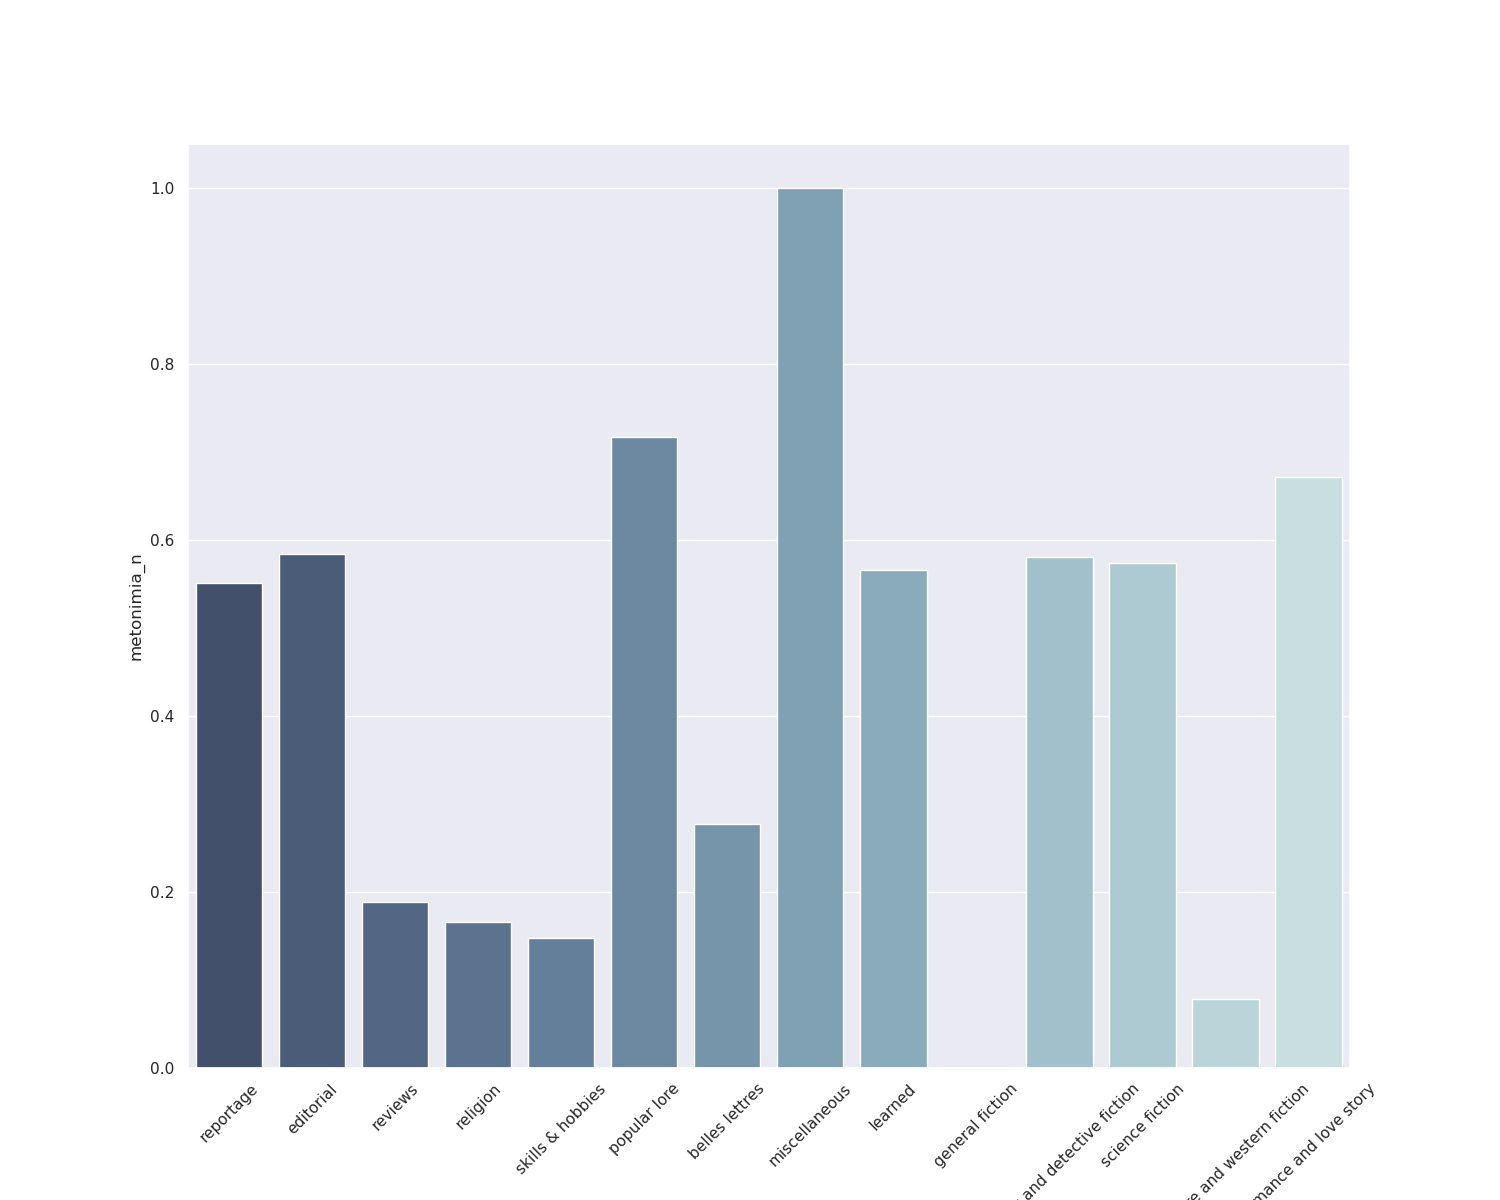
\includegraphics[width=.45\linewidth]{./resultados/graphs/muestra/c5_metonimia.png}
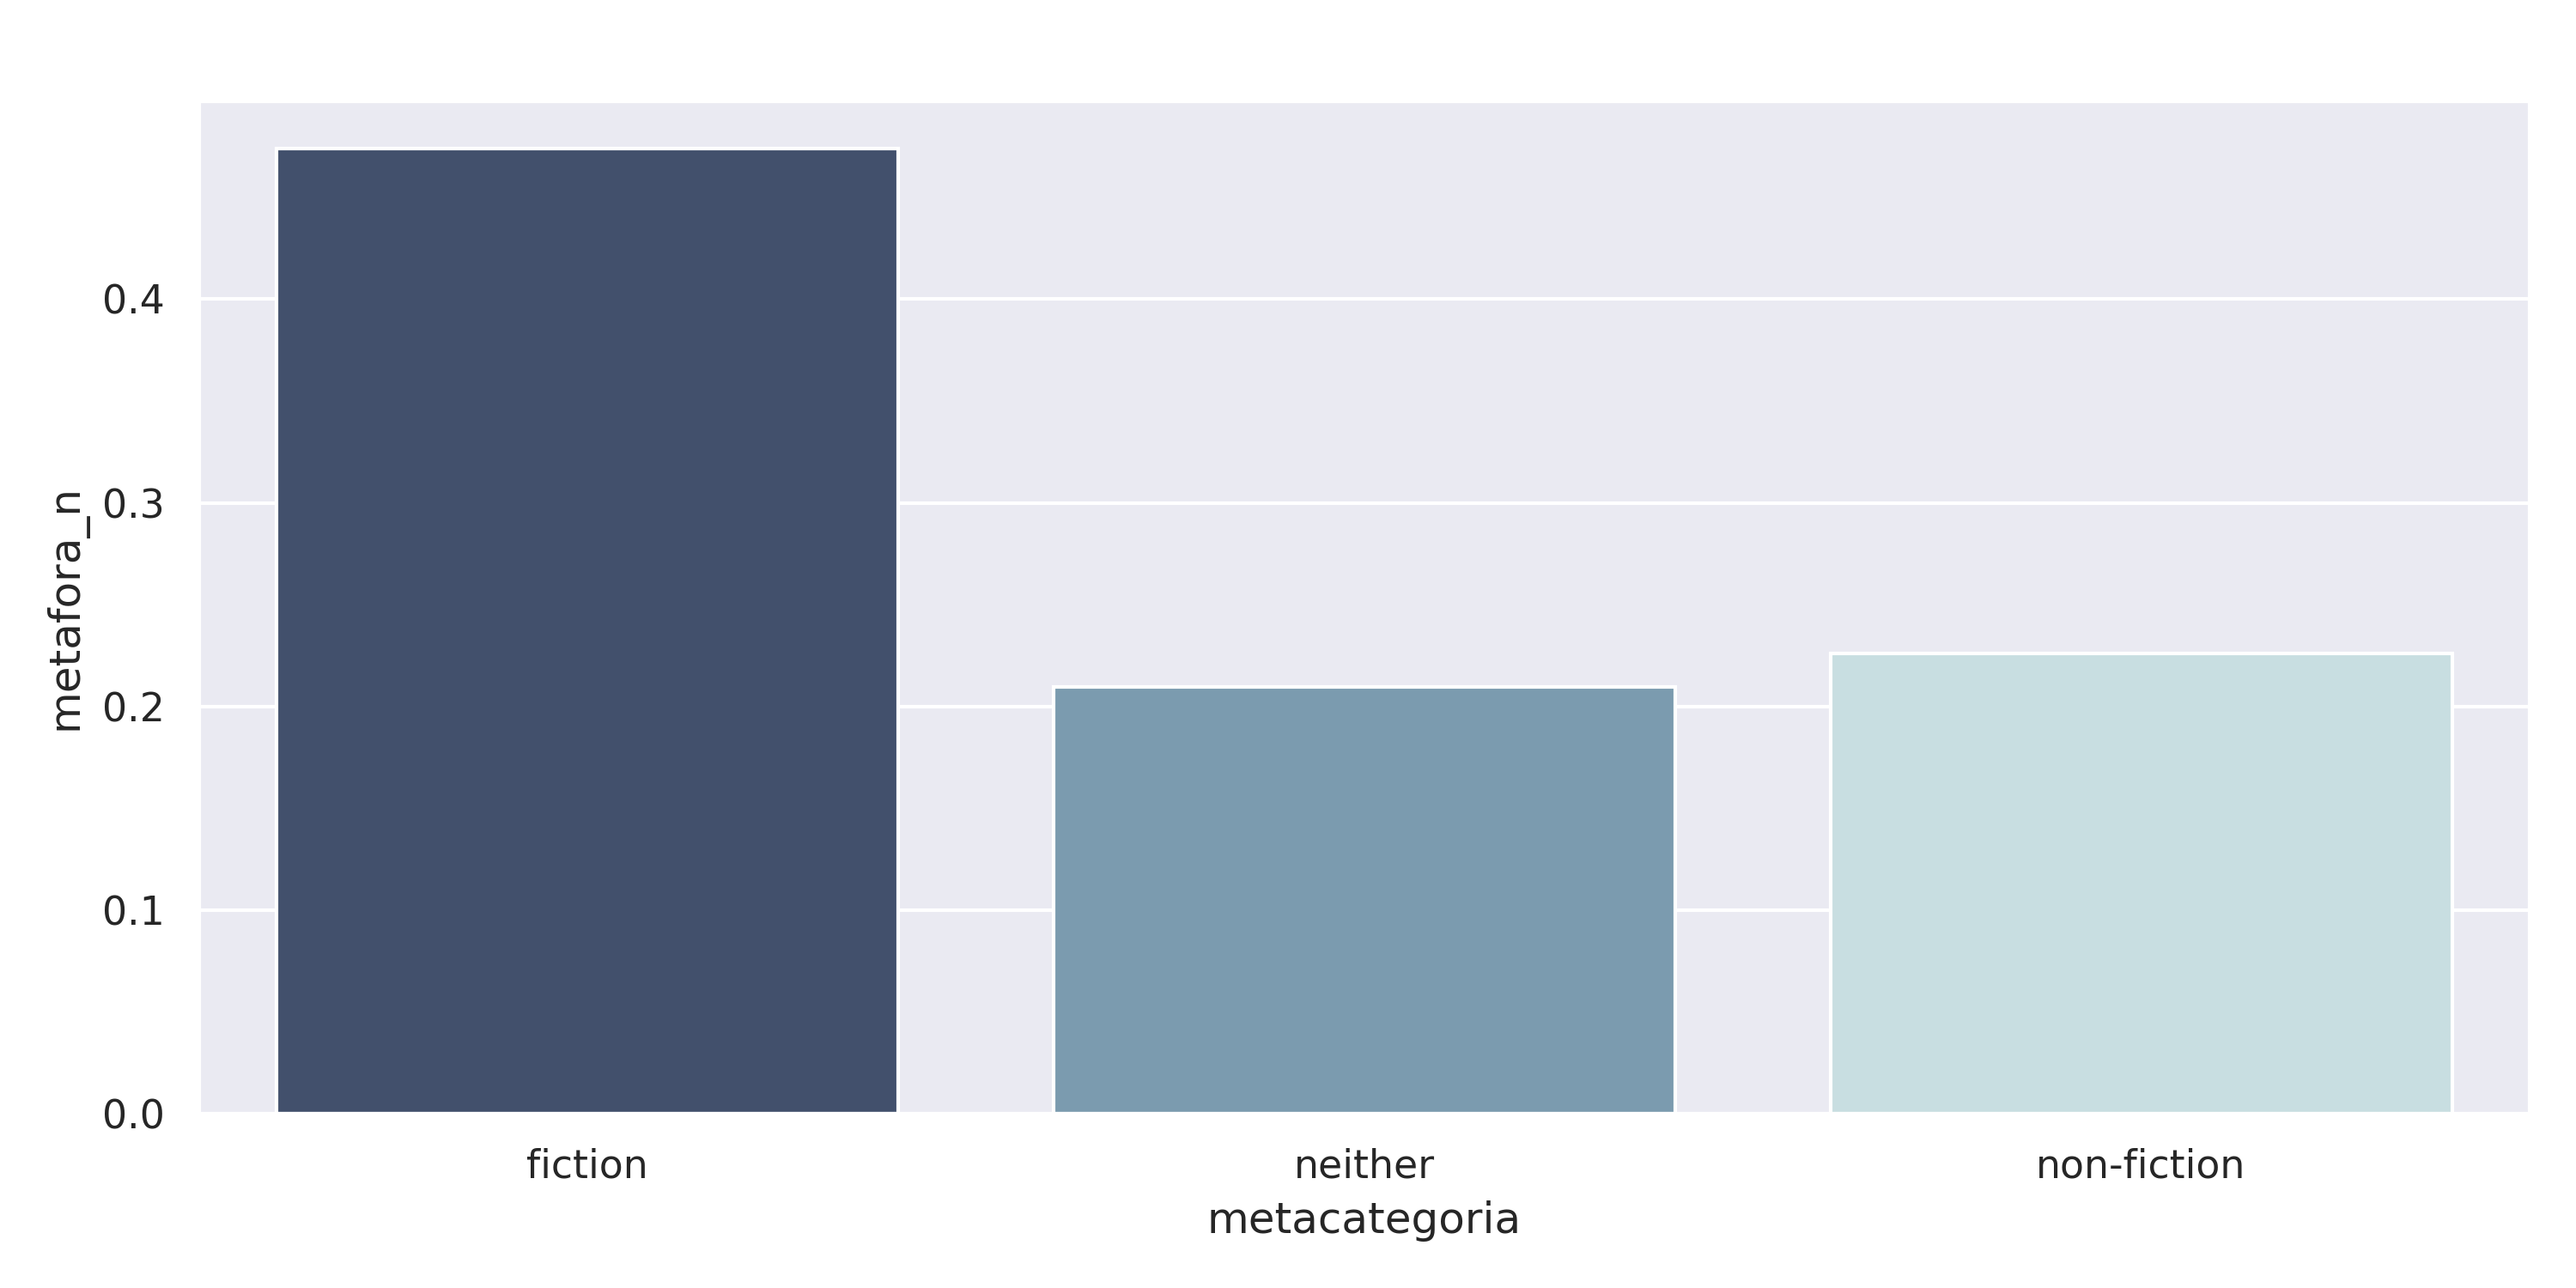
\includegraphics[width=.45\linewidth]{./resultados/graphs/meta/c5_metacategoria_metafora.png}
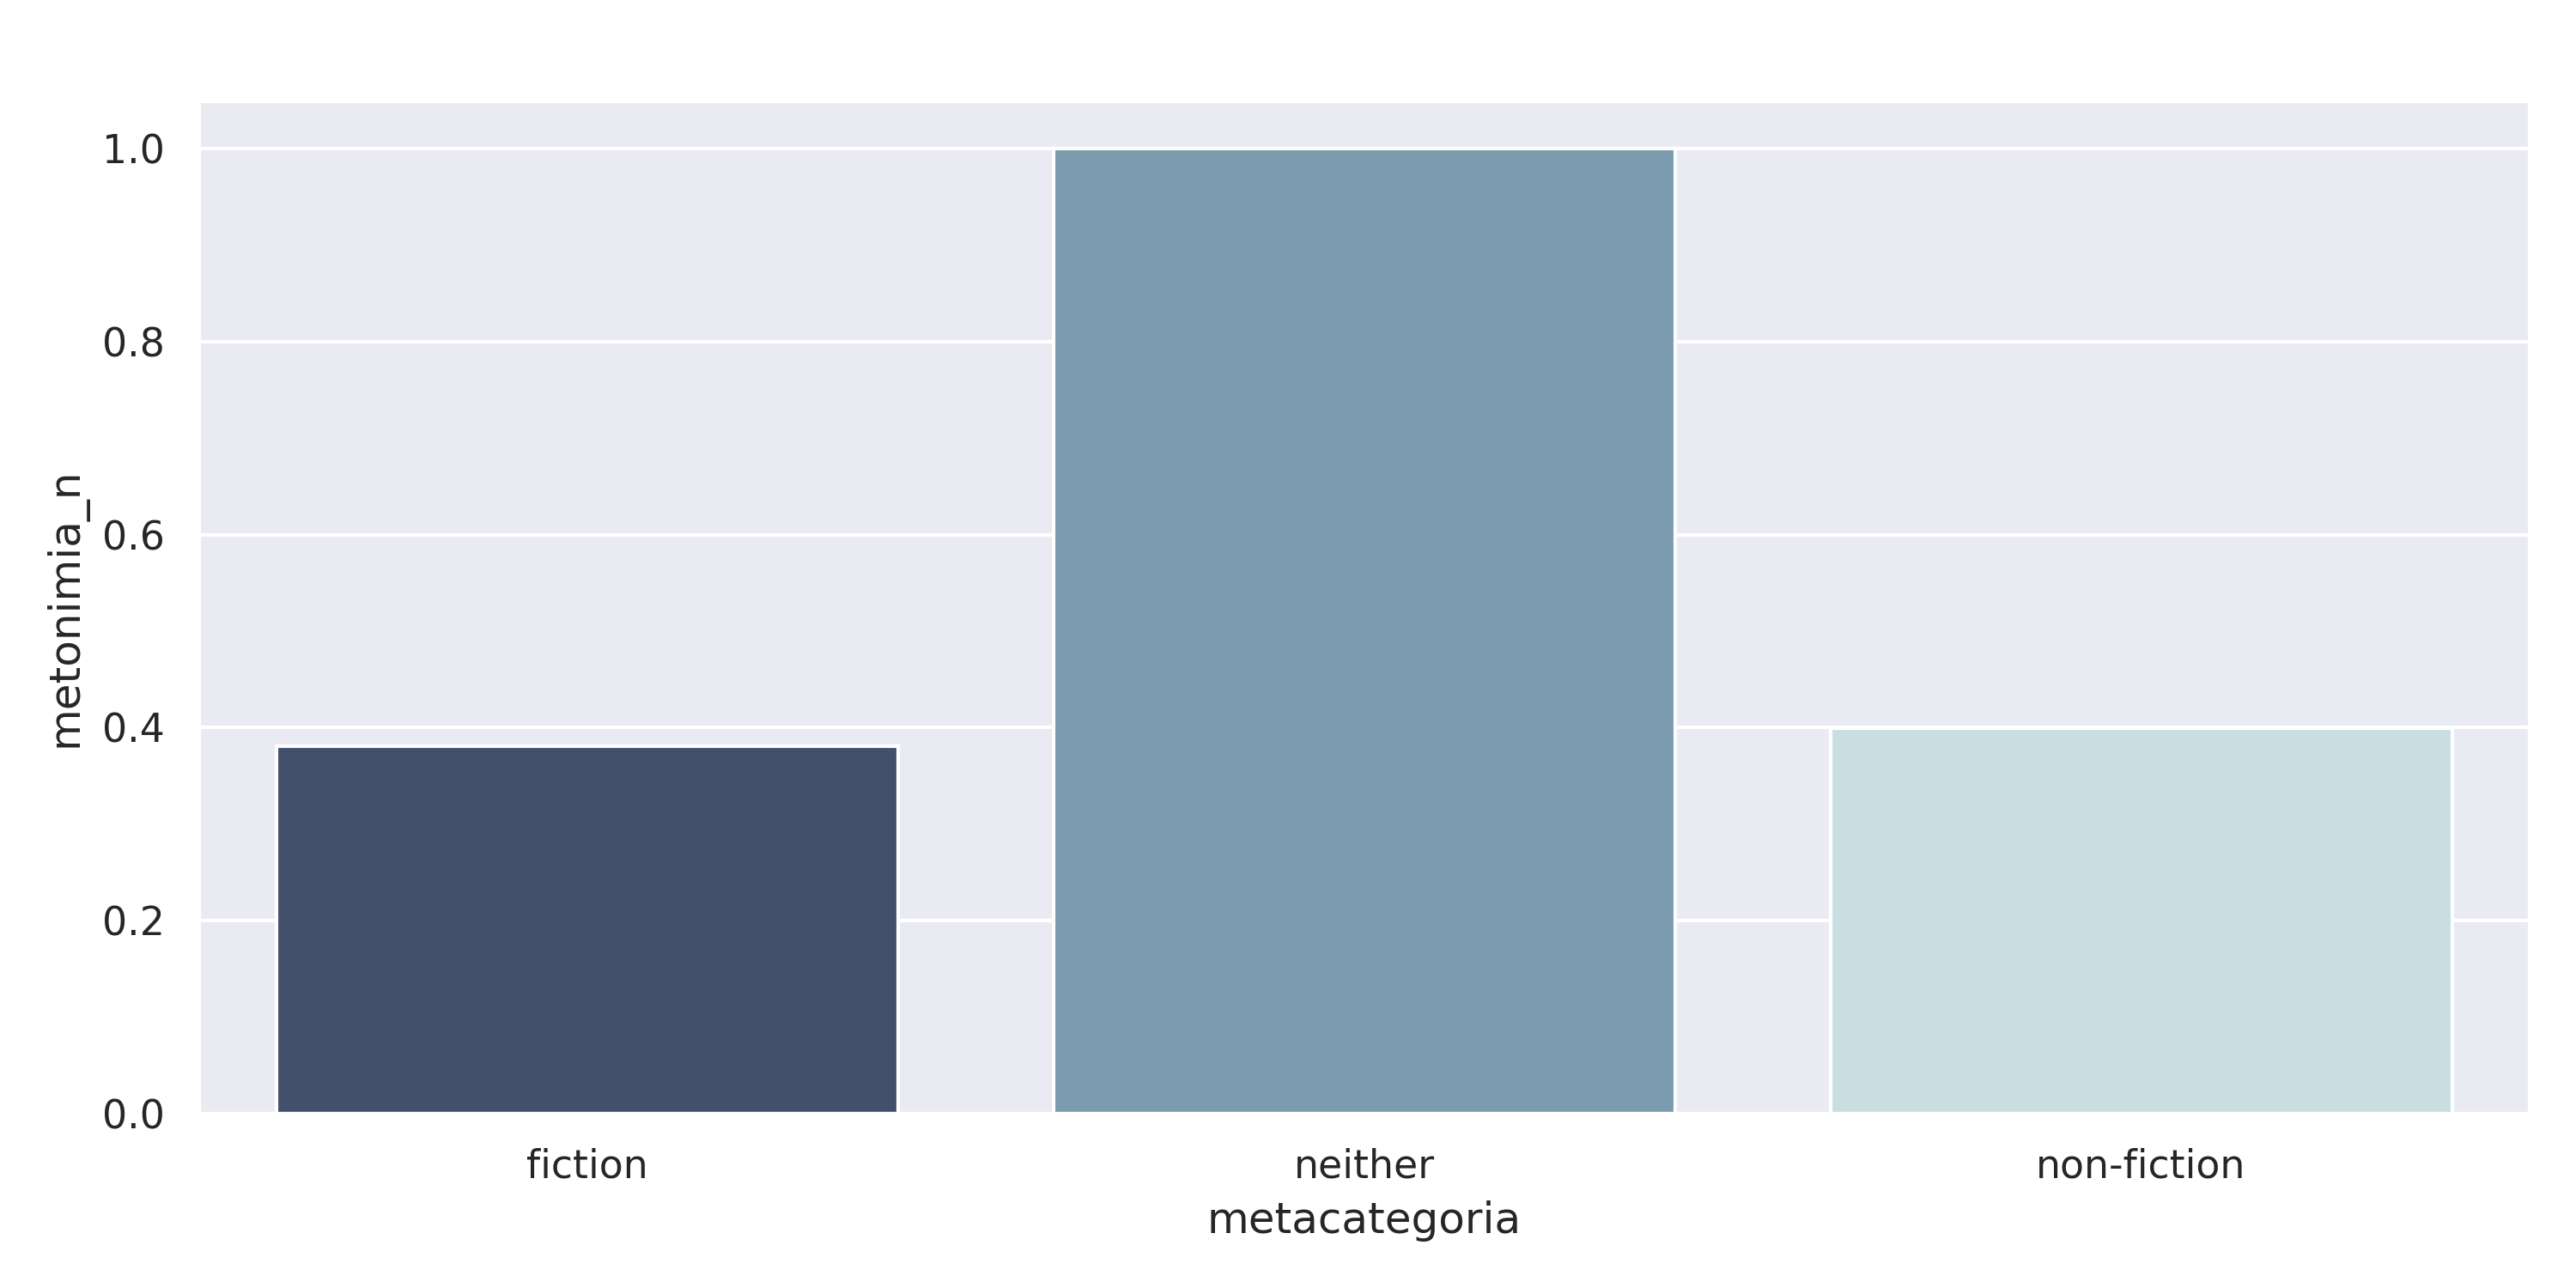
\includegraphics[width=.45\linewidth]{./resultados/graphs/meta/c5_metacategoria_metonimia.png}
\caption{\label{fig:c5_resultados}Resultados muestra 5}
\end{figure}


\subsubsection{Gráficos totales}
\label{sec:org40b5bf2}
\begin{figure}[!H]
\centering
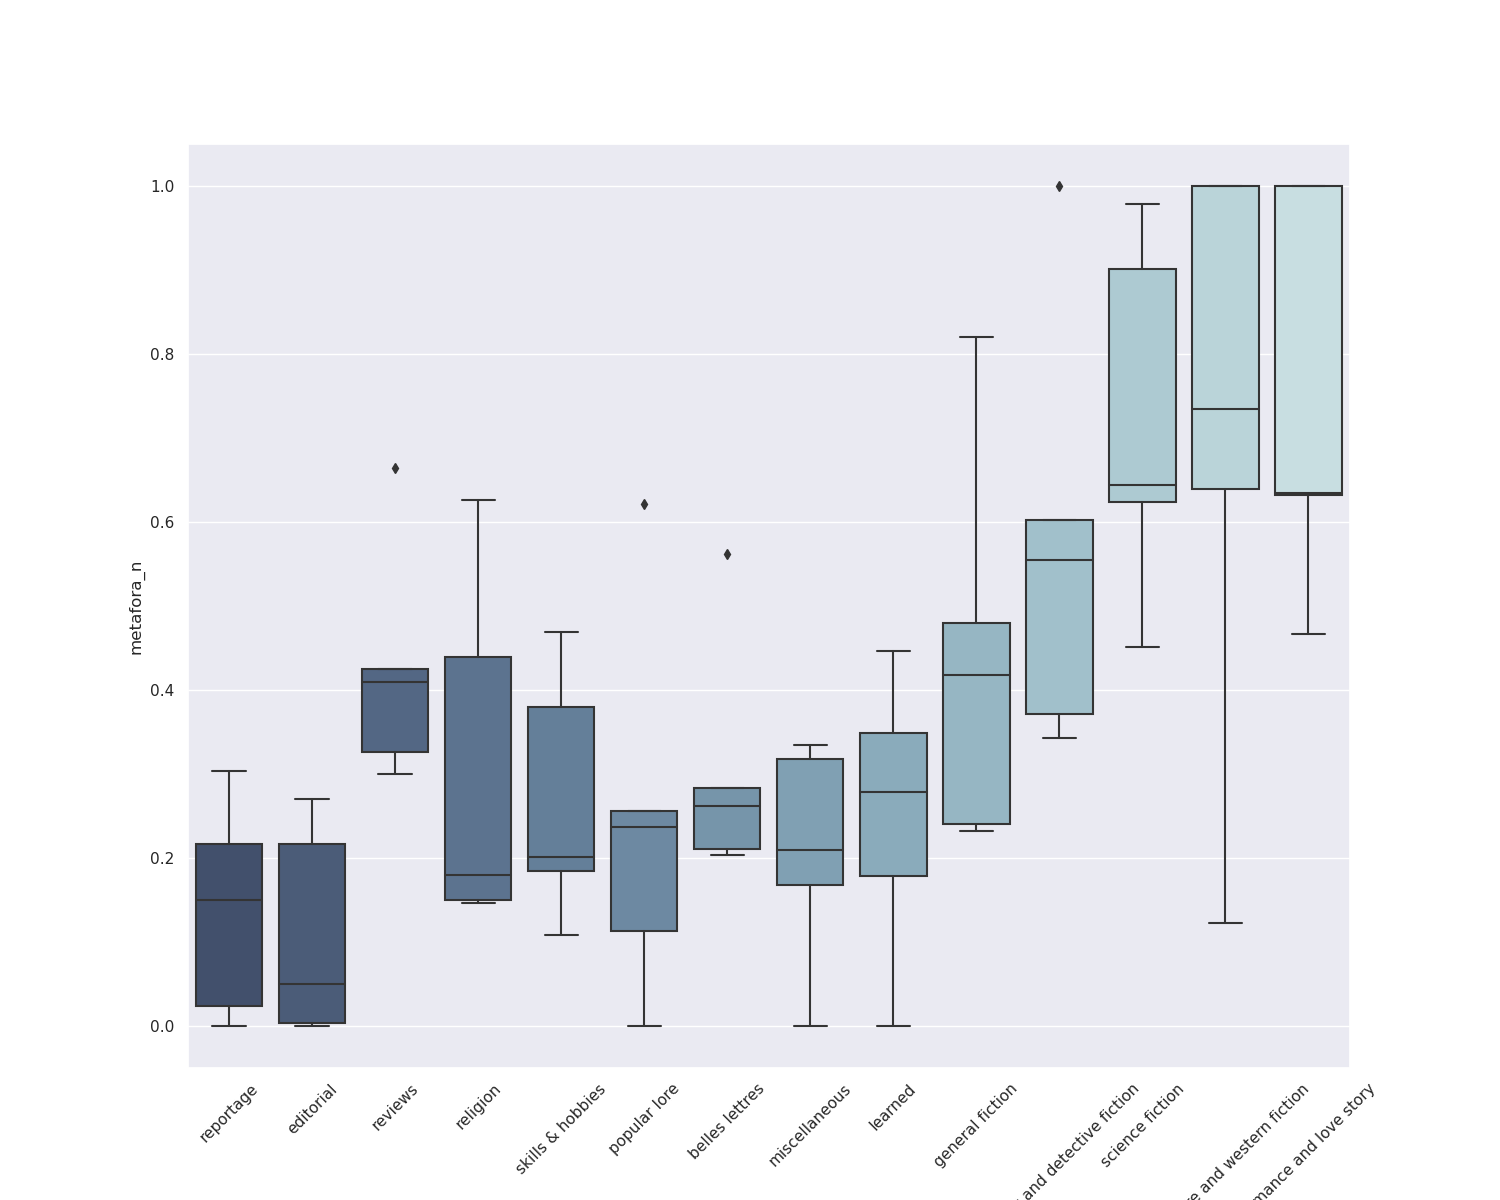
\includegraphics[width=0.9\linewidth]{./resultados/graphs/total/accum_cat_metafora.png}
\caption{\label{fig:metafora_categorias} Índice metafórico por categorías a través de las muestras }
\end{figure}
\begin{figure}[!H]
\centering
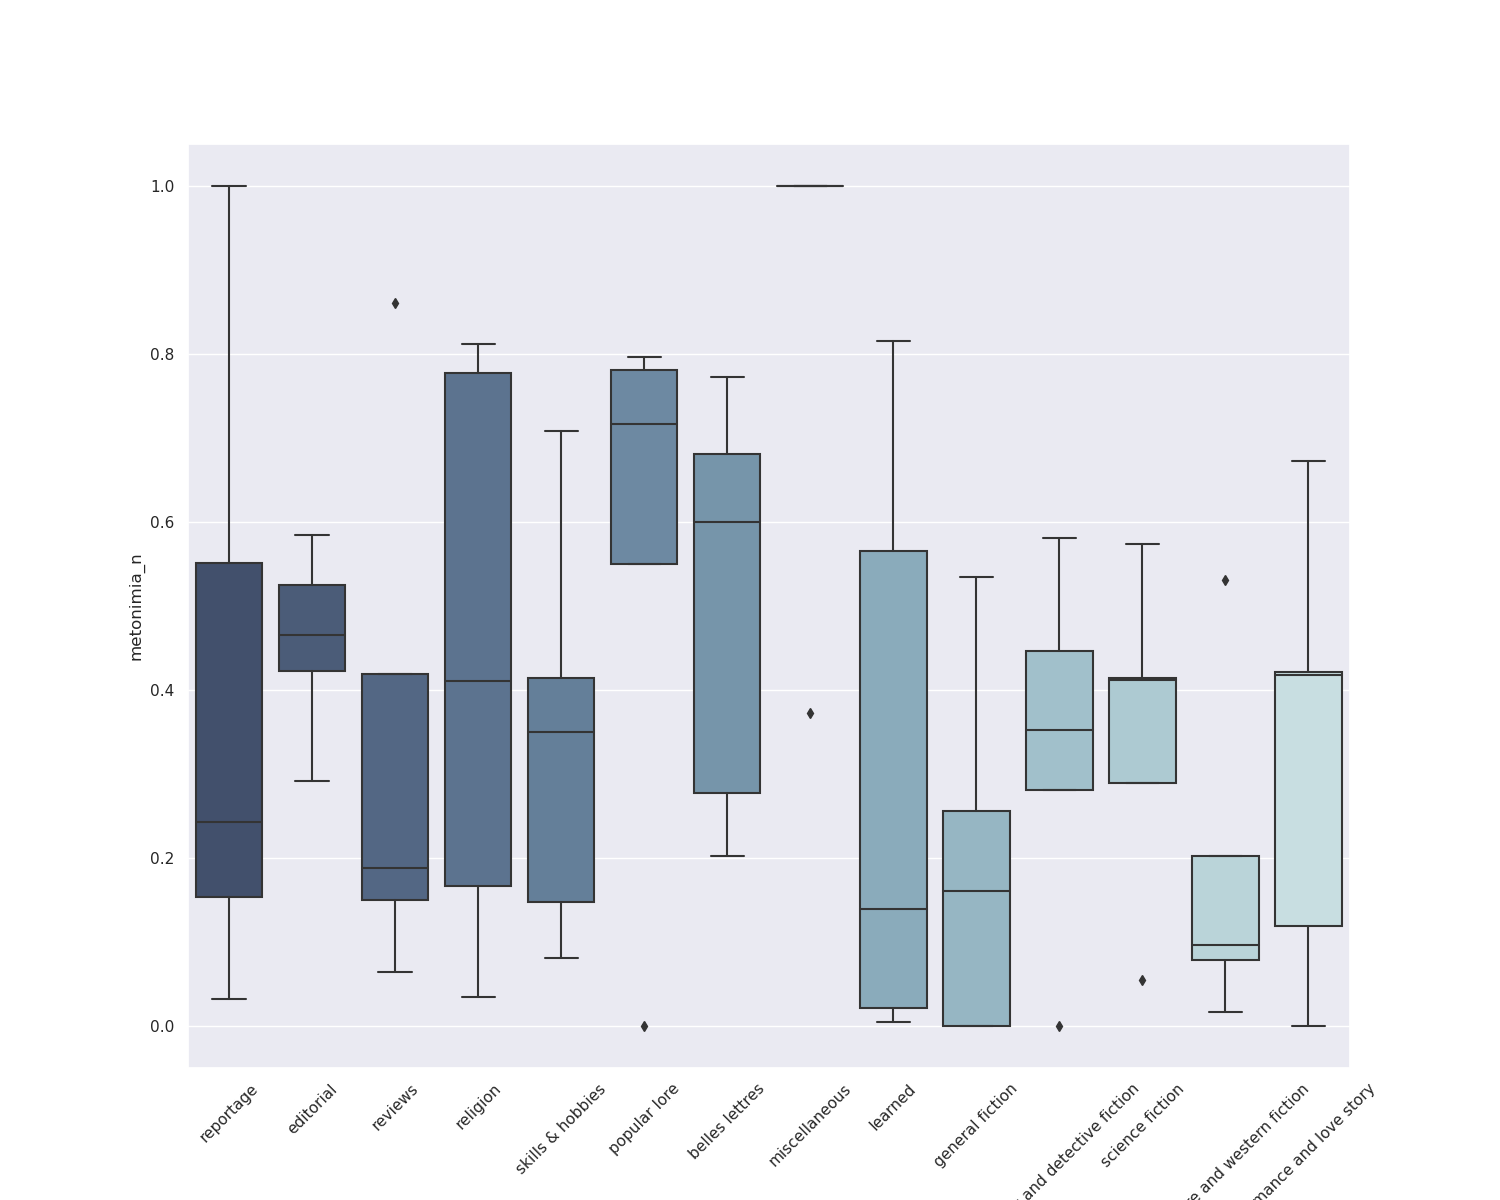
\includegraphics[width=0.9\linewidth]{./resultados/graphs/total/accum_cat_metonimia.png}
\caption{\label{fig:metonimia_categorias} Índice metonímico por categorías a través de las muestras  }
\end{figure}
\begin{figure}[!H]
\centering
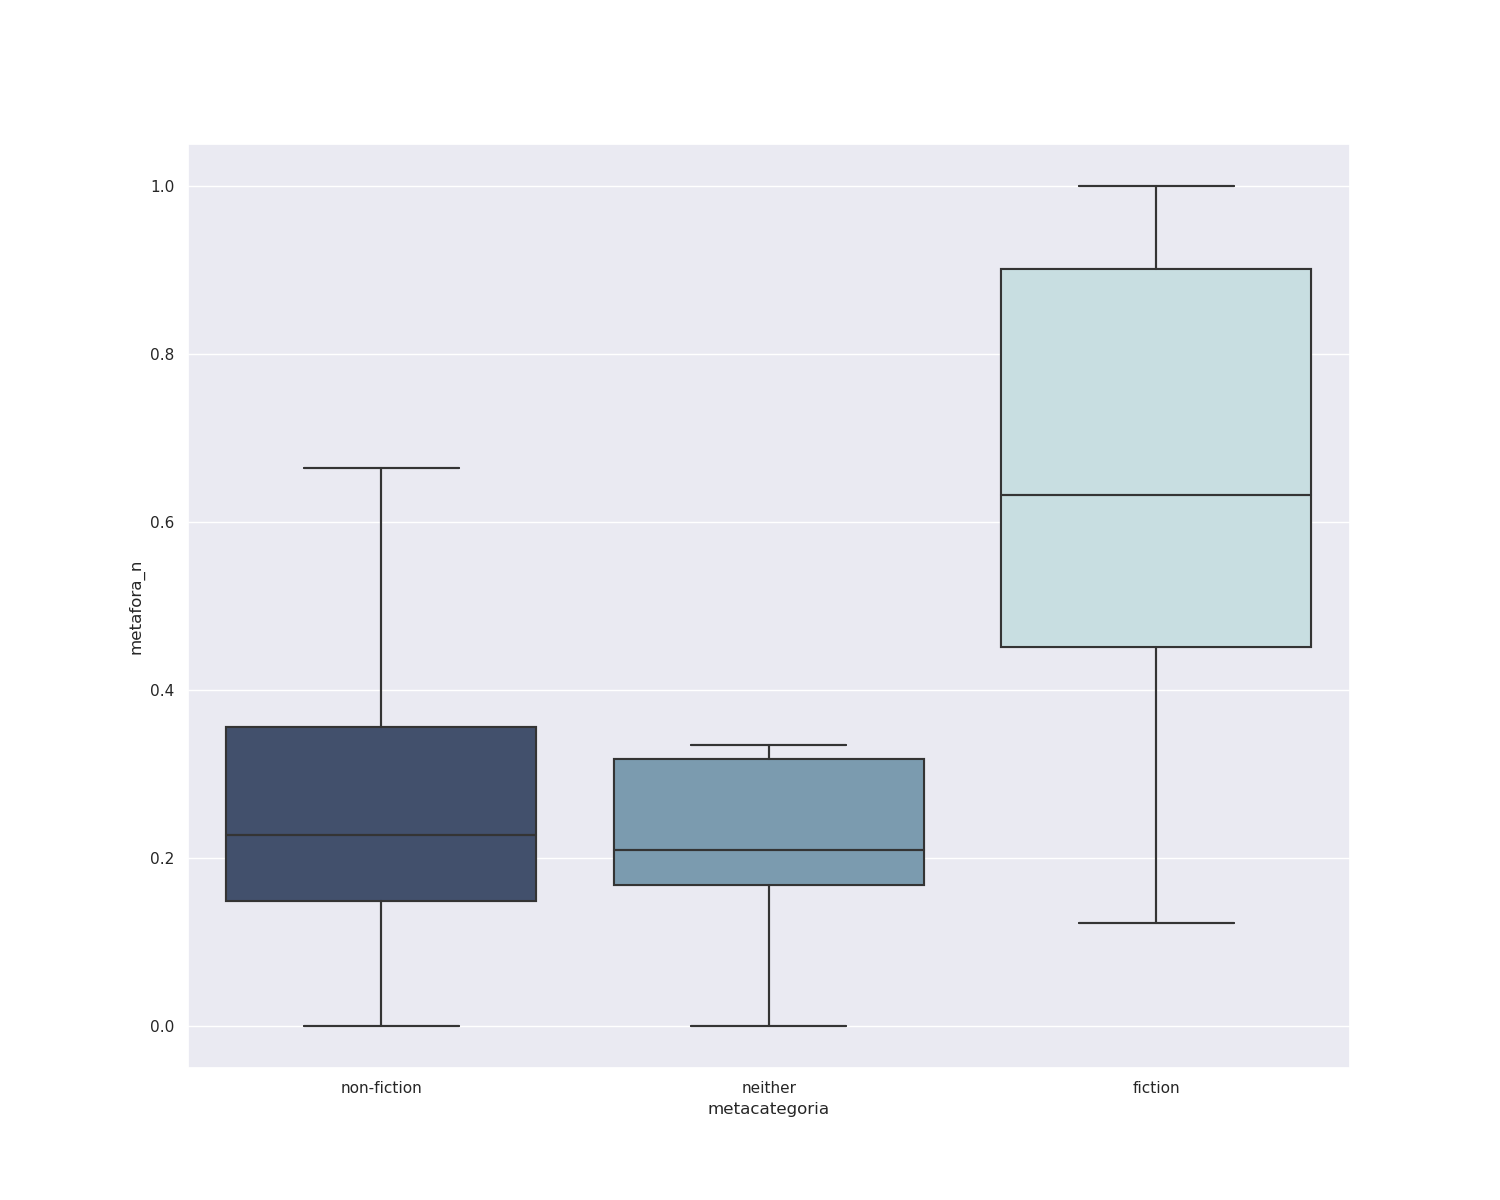
\includegraphics[width=0.9\linewidth]{./resultados/graphs/total/metafora_total.png}
\caption{\label{fig:metafora_total} Índice metafórico por metacategorías a través de muestras }
\end{figure}

\begin{figure}[!H]
\centering
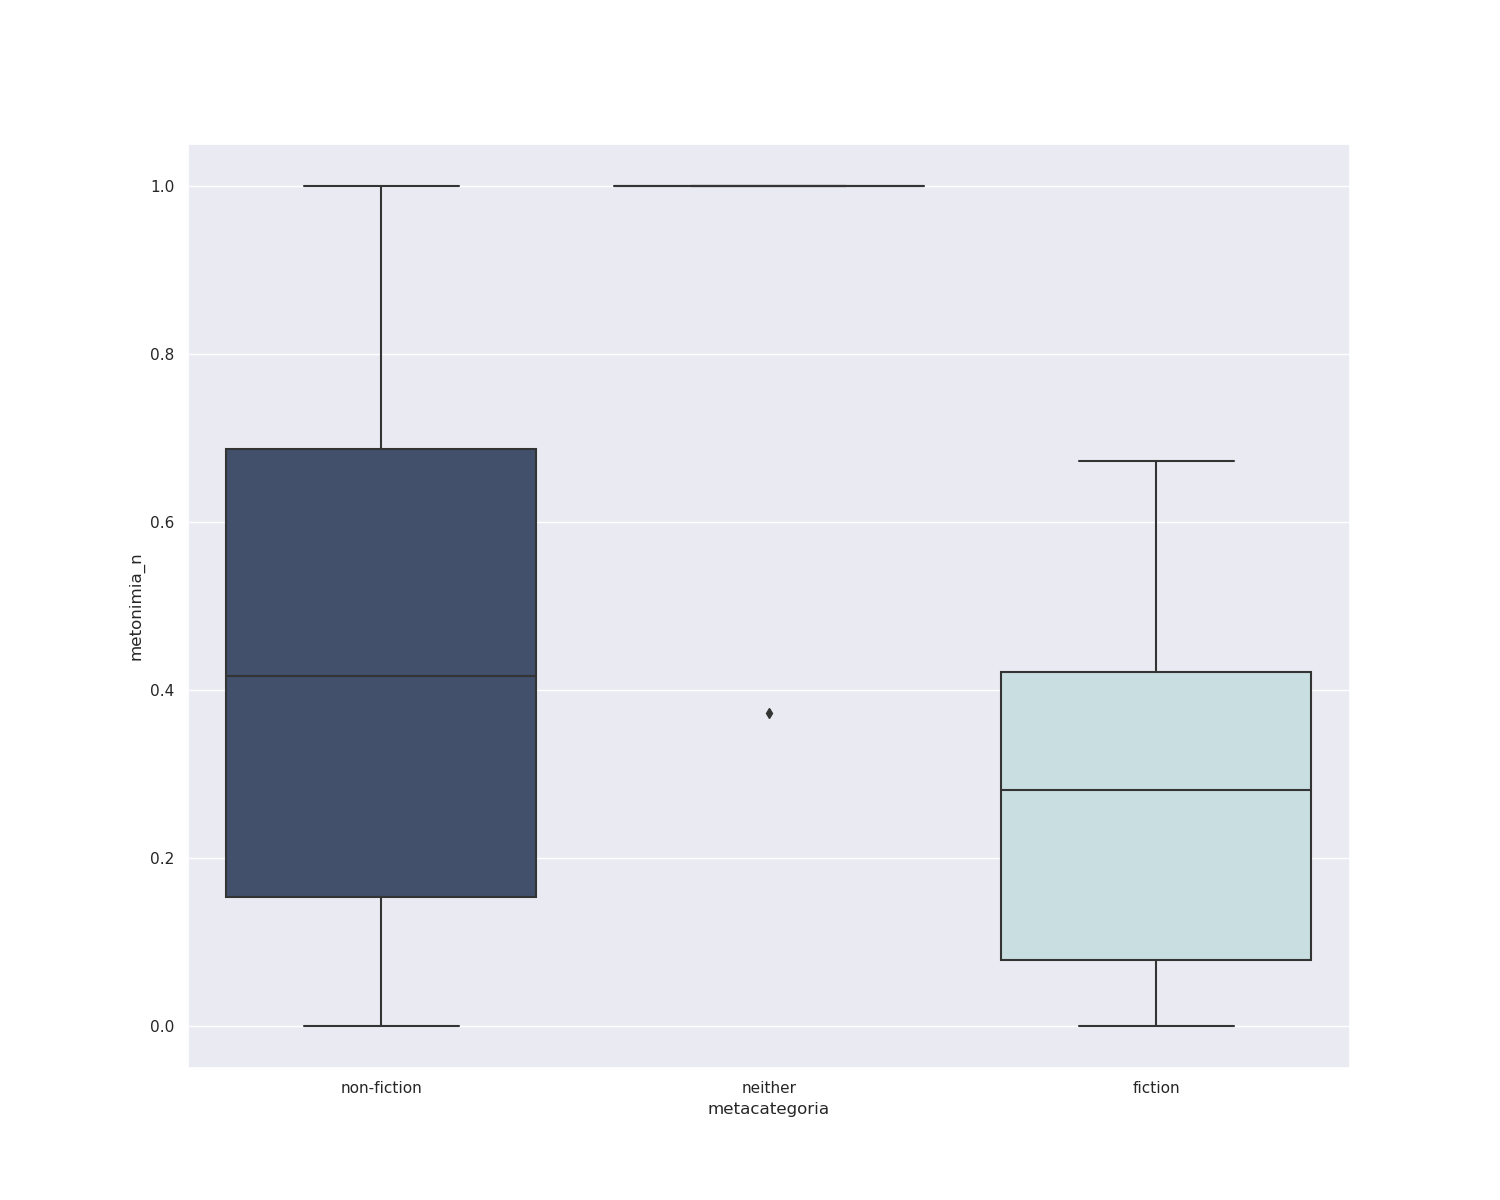
\includegraphics[width=0.9\linewidth]{./resultados/graphs/total/metonimia_total.png}
\caption{\label{fig:metonimia_total} Índice metonimica por metacategoria a través de muestras }
\end{figure}

\section{CONCLUSIONES}
\label{sec:org30c1460}

Para concluir el presente trabajo. Primero se señalarán los
resultados del experimento frente a las hipótesis planteadas.
Posteriormente, se expondrán las críticas posibles al modelo
planteado. Por último, se señalaran trabajos futuros para profundizar
más en la pregunta de investigación.

\subsection{Las hipótesis planteadas}
\label{sec:orga8c4e35}

Para la hipótesis H\textsubscript{1} se observa en \ref{fig:metafora_total} que el
índice metafórico es, en promedio, más alto para las categorias de no
ficción a lo largo la muestras que para las categorias de no
ficción. De hecho, en promedio, las obras de ficción reportan un
índice metafórico un poco más de 3 veces más alto. Esto es consistente
con la intuición, que nos dicta que en las obras de ficción se hace
uso de un vocabulario más amplio y distinguido, lo que aporta más al
índice metafórico.

En cuanto a la hipótesis H\textsubscript{2}, las medias para las categorias
\emph{reportage} y \emph{editorial} son cercabis (0.14 y 0.11,
respectivamente). En el gráfico \ref{fig:metafora_categorias} se puede
apreciar que el rango interquartil (IRQ) es muy similar. Esto es
consistente con el resultado esperado, puesto que estas dos categorías
son similares entre sí: ambas están conformadas por textos que
aparecieron en publicaciones periódicas. Por lo tanto, comparten
muchos parámetros linguísticos similares en cuanto al vocabulario. Por
lo tanto, sú indice metafórico debe ser similar a lo largo de las
muestras.

Luego, para la hipótesis H\textsubscript{3} se puede observar que la categoria
\emph{Belles Lettres} es la tercera más categoría con el índice metafórico
más alto (con un 0.30). Queda por debajo de \emph{Religion} (0.31) por un
punto y de \emph{Reviews} (0.42). Este resultado no es el esperado, pero es
comprensible si se tiene en cuenta que la categoría \emph{Reviews} está
compuesta de críticas a obras de arte como música clásica, libros y
obras de teatro, cuyo vocabulario puede terminar aportando más al
índice metafórico que las biografías y caras de la categoría \emph{Belles
Lettres}.

Por último, para la hipótesis H\textsubscript{4}, se observa que la categoría
\emph{Learned} tiene el segundo índice de metonimia más bajo (0.31), luego
de (sorprendentemente) las categorias \emph{General Fiction} y \emph{Adventure \&
Western Fiction} (0.19 ambas). Si bien este resultado no es
estrictamente el esperado a lo largo de todas las categorias, la
hipótesis H\textsubscript{4} sí se cumple dentro de la metacategoría de
no-ficción. La hipótesis inicial se hizo sobre la base de que los
textos técnicos y científicos no deberían tener un enfasis en la
metonimia entre cada una de sus palabras.  Es decir, no debería haber
un énfasis en repetir sonidos a lo largo de una oración, puesto que
los factores de comunicación de Jakobson se centran en las funciones
conativa o fática.

Ahora bien, en la hipótesis inicial no se contemplo que, según lo
encontrado en este experimento, las obras de ficción por lo general
tienen un índice metonímico más bajo que las de no ficción (ver \ref{fig:metonimia_total}. Esto
parece apuntar a una relación inversa entre el índice metaforico
y el índice metonómico. Sin embargo, esa discusión está por fuera
de los alcances de la presente investigación.


Con base en el análisis de las hipótesis, se puede señalar que
el algoritmo propuesto es capaz de:

\begin{itemize}
\item 'distinguir' entre dos metacategorias: los textos de ficción y los de no ficción
\item arrojar un índice metaforico consistentemente más alto que los de no-ficción para los textos de ficción
\item arrojar, para los textos de no ficción, un índice metonímico consistentemente mas alto que los de ficción
\end{itemize}

\subsection{Crítica del modelo}
\label{sec:orga36078d}


En términos generales, se considera que el modelo es razonablemente exitoso. En general no
hay resultados inconsistentes con la intuición, salvo el comportamiento del índice metonimico
a lo largo de una categoria. Sin embargo, si se considera las metacategorias de ficción y no
ficción, en la muestras se evidencia claramente que hay una consistencia en los resultados.

Una debilidad significativa del modelo es su dependencia de la con la red semántica. Esto
ocasiona que dada una palabra, su vector semantico quede asociado con palabras muy dificiles de
encontrar,lo que incide en su puntuación total. Esto particularmente se evidencia en algunas palabras
comunes que no se encuentran tan solo porque son pronombres o adverbios que empiezan con mayúscula
cuando la red los espera en minúscula. Es posible que esto esté afectando el modelo, pero no es claro
a priori de qué manera lo hace porque se haría necesario un análisis multivariado para cada una de las
variables. Ahora bien, esta falencia no parece ser tan pronunciado, ya que la diferencia entra las metacategorias
es evidente y resulta inverosímil atribuir la concordancia con la intuición y el juicio experto a un mero error.

Sin embargo, para tener una fundamentación más rigurosa de la idoneidad del algoritmo se debe diseñar un
experimento que mire los resulados de cada vector de uso por palabra y verificar como el número de sinónimos,
la media de esos sinónimos y la frecuencia de la palabra original en los corpus se compartan. Una tarea que no es
fácil por la dependencia de las variables de otras. Este aspecto es muy importante hacerlo, pero se sale de los
alcances de esta investigación. 



\subsection{Trabajo futuro}
\label{sec:orgf3d57f4}

\subsubsection{El índice metafórico}
\label{sec:org45e01bb}
Para trabajos futuros es necesario repetir más veces este mismo experimento, aumentando el número de muestras.
Luego, se podría plantear el mismo documento con un corpus distinto, tal vez con categorias individuales
distintas, pero conservando las mismas metacategorías:ficción y no ficción. Si el resultado sigue
avalando la hipótesis H\textsubscript{1} fortalecería la validez del modelo para capturar la 'metafora' en documentos.

Por otro lado, como se expuso en el marco teórico y en la presentación del modelo, el índice metafórico
es dependiende del corpus de referencia, que es una representación del concepto de \emph{lengua}, y la
red semántica, que corresponde con el concepto de \emph{lenguaje}. Así, para obtener resultados más
intuitivos se deberá disponder de la capacidad de configurar tanto el corpus de referencia como la
red semántica. Por ejemplo, para asociar palabras entre sí en la red semántica o quitar relaciones
espurias.


\subsubsection{El índice metonímico}
\label{sec:org610eacd}

El algoritmo para metonimia fue realizado de la manera más \emph{naive} posible, lo que puede ser una causa
de la variabilidad de este índice entre una misma categoria a lo largo de las muestras. Un siguiente
paso sería calcular la metonimia no por el número de letras iguales, sino tokenizar por sílabas y contar
las sílabas con una misma vocal como un aporte al índice.

Otra posible modificación es parametrizar el la aridad del n-grama, puesto que la repetición de sonidos
solo se está teniendo en cuenta para palabras consecutivas, cuando en realidad la metonimia suele darse
por elementos sintacticos distintos. Por ejemplo, se puede dar entre oraciones, ente párrafos, entre estrofas
etc. Sin embargo, el cálculo de esto necesitaria incorporar POS al modelo, lo que complejizaría significativamente
la implementación del índice. 



\bibliographystyle{unsrt}
\bibliography{biblio} 
\end{document}